
\documentclass[12pt,twoside]{book}
\usepackage[utf8]{inputenc} 
\usepackage[T1]{fontenc}   
\usepackage{lmodern} 
\usepackage[brazil]{babel}
\usepackage{tikz}
\usetikzlibrary{positioning,arrows.meta}
\usepackage[ruled]{algorithm2e}
\renewcommand{\listalgorithmcfname}{Lista de Algoritmos}%
\renewcommand{\algorithmcfname}{Algoritmo}%

%\usepackage{subfigure}
\usepackage{subfloat}

%%% acentuação
% \usepackage[latin1]{inputenc}
% \usepackage[brazil]{babel}

%%% bibliografia
%\usepackage{chicago}
\usepackage[round]{natbib}
\bibliographystyle{apalike}
\newcommand{\citeay}[1]{\citeauthor{#1}, \citeyear{#1}}

% \usepackage[alf]{abntex2cite}
% \bibliographystyle{abntex2-alf}

\usepackage{latexsym}


\usepackage{setspace}
% \usepackage{mathptm}
\usepackage{latexsym}
\usepackage{amssymb}
\usepackage{xspace}
\usepackage{colortbl}

\usepackage{acronym}
%%% referencias com página \vref
\usepackage[brazil]{varioref}

%%% identa primeiro parágrafo
\usepackage{indentfirst}

%%% figuras um ao lado do outro
\usepackage{subfig}


%%% definir títulos de seção
\usepackage[sf,sl,outermarks]{titlesec}


%%% para tabelas
\usepackage{multirow}

%%% boxes
\usepackage{fancybox}
\usepackage{fancyvrb}
\usepackage{color}

%%% somente na versão PDF

%%% Para inclusão de gráficos
%\usepackage[pdftex]{graphicx}
\usepackage{graphicx}

%%% dimensões do documento
\usepackage[pdftex]{geometry}
  \geometry{a4paper,left=3cm,right=2cm,top=2.0cm,bottom=2cm,twoside}

%%% cria links no arquivo .pdf
%%% comentar as linhas na versão para impressao
\usepackage[pdftex,pdfpagelabels,pagebackref]{hyperref}
%\usepackage{hyperref}


%%% propriedades do arquivo .pdf
\hypersetup{
    pdftitle = {},
    pdfsubject = {},
    pdfkeywords = {},
    pdfauthor = {}
    }


\hypersetup{colorlinks=true,linkcolor=black,citecolor=black,hypertexnames=false}

%%fonte
\usepackage{bookman}
\usepackage[T1]{fontenc}

%%para os numeros reais
\usepackage{amsfonts}
\usepackage{amsmath}

\DeclareFixedFont{\numberfont}{T1}{phv}{bx}{n}{2cm}

%%% redefine o formato do título



\titleformat{\chapter}[display]
  {\normalfont\Large\sffamily
  }
  {%\titlerule[3pt]%
   \filright
   \rule[32pt]{.7\linewidth}{4pt}
   \hspace{-11pt}
   \shadowbox{
   \begin{minipage}{.18\linewidth}
     \begin{center}
       \textsc{\Large\chaptertitlename}\\
       \vspace{1ex}
       {\numberfont\color[gray]{0.5} \thechapter}\\
       \vspace{1ex}
     \end{center}
   \end{minipage}}
  }
  {0pt}
  {\filcenter
   \Huge
   }
  [\hfill\rule{.8\textwidth}{0.5pt}\\
     \vskip-1.8ex\hfill\rule{.7\textwidth}{3pt}]


%%% macro para destacar a(s) primeira(s) letra do texto
%%% é necessário ter a fonte courier instalada
%
%  um texto do tipo:
%
%  \begin{document}
%    \versal{IN} THE beginning God created the heaven and the earth.  Now the
%    earth was unformed and void, and darkness was upon the face of the
%    deep; and the spirit of God hovered over the face of the waters.
%  \end{document}
%
%  irá produzir algo como:
%
%  I I\  I THE beginning God  created the heaven and  the earth.
%  I I \ I Now the earth was unformed and void, and darkness was
%  I I  \I upon the face of the deep; and the spirit of God hov-
%  ered over the face of the waters.

%\font\largefont= pzcmi scaled 6500

\newcommand{\versal}[1]{{\noindent
    \setbox0\hbox{\largefont #1 }%
    \count0=\ht0                   % height of versal
    \count1=\baselineskip          % baselineskip
    \divide\count0 by \count1      % versal height/baselineskip
    \dimen1 = \count0\baselineskip % distance to drop versal
    \advance\count0 by 1\relax     % no of indented lines
    \dimen0=\wd0                   % width of versal
    \global\hangindent\dimen0      % set indentation distance
    \global\hangafter-\count0      % set no of indented lines
    \hskip-\dimen0\setbox0\hbox to\dimen0{\raise-\dimen1\box0\hss}%
    \dp0=0in\ht0=0in\box0}}
% Backref com colocação de "Citado na página..."
\renewcommand*{\backref}[1]{}
\renewcommand*{\backrefalt}[4]{
   \ifcase #1
       Não citado no texto.
   \or
       Citado na página~#2.
   \else
       Citado nas páginas #2.
   \fi
}

\renewcommand{\backreftwosep}{ e~}
\renewcommand{\backreflastsep}{, e~}


\usepackage{pgf}
\usepackage{baseboxes}
\usepackage{basecolor}


\begin{document}

\newcommand{\natr}{{n_{at}}}
\newcommand{\nexe}{{n_{ex}}}
\newcommand{\ncls}{{n_{cl}}}
\newcommand{\nseg}{{n_{sg}}}
\newcommand{\di}{{D_1}}
\newcommand{\dii}{{D_2}}



\newcommand{\palestra}{\textit{palestra}\xspace}
\newcommand{\relevancia}{\hbox{\textit{relevância}}}
\newcommand{\distancia}{\hbox{\textit{distância}}}
\newcommand{\comida}{\hbox{\textit{comida}}}
\newcommand{\brinde}{\hbox{\textit{brinde}}}

\newcommand{\rankeadores}{\textit{rankeadores}\xspace}
\newcommand{\rankeador}{\textit{rankeador}\xspace}
\newcommand{\rankings}{\textit{rankings}\xspace}
\newcommand{\ranking}{\textit{ranking}\xspace}
\newcommand{\classificadorScore}{classificador \textit{score}\xspace} 
\newcommand{\classificadoresScore}{classificadores \textit{score}\xspace}
\newcommand{\estimadorProbabilidade}{\textit{estimador de probabilidade}\xspace} 
\newcommand{\estimadoresProbabilidade}{\textit{estimadores de probabilidade}\xspace} 
\newcommand{\segmento}{\textit{segmento}\xspace}
\newcommand{\segmentos}{\textit{segmentos}\xspace}
\newcommand{\adjacente}{\textit{adjacente}\xspace}
\newcommand{\adjacentes}{\textit{adjacentes}\xspace}
\newcommand{\grosseiro}{\textit{grosseiro}\xspace}
\newcommand{\refinado}{\textit{refinado}\xspace}

\newcommand{\overfitting}{\textit{overfitting}\xspace}


\newcommand{\jfe}{\textit{J48}\xspace}
\newcommand{\cfourfive}{\textsc{C4.5}\xspace}
\newcommand{\lexrank}{\textsc{LexRank}\xspace}
\newcommand{\lexprob}{\textsc{LexProb}\xspace}
\newcommand{\calinb}{\textsc{CaliNB}\xspace}

\newcommand{\progroc}{\textsc{ProgROC}\xspace}
\newcommand{\cotraining}{\textsc{Co-training}\xspace}
\newcommand{\corai}{\textsc{Corai}\xspace}
\newcommand{\nb}{\textsc{naive Bayes}\xspace}
\newcommand{\ie}{\textit{i.e.}\xspace}

\newcommand{\mc}{\hbox{\textit{c}}}
\newcommand{\mvp}{\hbox{\textit{VP}}}
\newcommand{\mfp}{\hbox{\textit{FP}}}
\newcommand{\mfn}{\hbox{\textit{FN}}}
\newcommand{\mvn}{\hbox{\textit{VN}}}

\newcommand{\mpos}{\hbox{\textit{Pos}}}
\newcommand{\mneg}{\hbox{\textit{Neg}}}

\newcommand{\mppos}{\hbox{\textit{PPos}}}
\newcommand{\mpneg}{\hbox{\textit{PNeg}}}

\newcommand{\mtotal}{\hbox{\textit{Total}}}

\newcommand{\mtvp}{\hbox{\textit{TVP}}}
\newcommand{\mtfp}{\hbox{\textit{TFP}}}

\newcommand{\tvp}{\textit{TVP}\xspace}
\newcommand{\tfp}{\textit{TFP}\xspace}

\newcommand{\vp}{\textit{VP}\xspace}
\newcommand{\fp}{\textit{FP}\xspace}
\newcommand{\fn}{\textit{FN}\xspace}
\newcommand{\vn}{\textit{VN}\xspace}


\newcommand{\ipos}{\textit{Pos}\xspace}
\newcommand{\ineg}{\textit{Neg}\xspace}


\newcommand{\total}{\textit{Total}\xspace}

\newcommand{\score}{\textit{score}\xspace}
\newcommand{\scores}{\textit{scores}\xspace}
\newcommand{\stm}{\textit{steamming}\xspace}

\newcommand{\stems}{\textit{stems}\xspace}
\newcommand{\stem}{\textit{stem}\xspace}

\newcommand{\precisao}{\textit{precisão}\xspace}
\newcommand{\oddsratio}{\textit{odds ratio}\xspace}
\newcommand{\posteriorodds}{\textit{posterior odds}\xspace}



\newtheorem{theorem}{Teorema}[chapter]
\newtheorem{corollary}[theorem]{Corolário}
\newtheorem{definition}{Definição}[chapter]
\newtheorem{example}{Exemplo}[chapter]


\newcommand{\chat}{\mbox{$\hat{c}$}}
\newcommand{\rhat}{\mbox{$\hat{r}$}}
\newcommand{\shat}{\mbox{$\hat{s}$}}
\newcommand{\phat}{\mbox{$\hat{P}$}}
\newcommand{\mhat}{\mbox{$\hat{m}$}}
\newcommand{\ghat}{\mbox{$\hat{g}$}}
\newcommand{\x}{\mbox{\textbf{x}}}
\newcommand{\nkp}{n_k^+}
\newcommand{\nkn}{n_k^-}

\newcommand{\adviolator}{\textit{adjacent violator}\xspace}
\newcommand{\adviolators}{\textit{adjacent violators}\xspace}

\newcommand{\gram}{gram\xspace}
\newcommand{\grams}{\textit{grams}\xspace}
\newcommand{\cbr}{\textsc{cbr}\xspace}
\newcommand{\ilp}{\textsc{ilp}\xspace}



\newcommand{\pretext}{\textsc{PreTexT}\xspace}
\newcommand{\news}{{\sc news}\xspace}
\newcommand{\course}{{\sc course}\xspace}
\newcommand{\lnai}{{\sc lnai}\xspace}
\newcommand{\ccourse}{{\tt course}\xspace}
\newcommand{\cncourse}{{\tt non-course}\xspace}
\newcommand{\sci}{{\tt sci}\xspace}
\newcommand{\talk}{{\tt talk}\xspace}
\newcommand{\texto}{\textsc{text}\xspace}
\newcommand{\links}{\textsc{links}\xspace}


\newcommand{\nni}{\textsc{9nni}\xspace}
\newcommand{\mode}{\textsc{mode}\xspace}


\newcommand{\brierScore}{\textit{Brier score}\xspace}


\pagestyle{empty}
\pagenumbering{roman}

%%% insere a capa
%%% edite os campos para título, data, orientador e nome

\newcommand{\titulo}{Desenvolvimento de Sistema Embarcado para Aquisição e Transmissão de Sinais de ECG em Redes LoRaWAN }
  

\begin{titlepage}




% \begin{center}
% \begin{minipage}[c]{12cm}
% \begin{center}
% \hrulefill\\
% \vspace{0.5cm}{\Large \titulo}\\
% \vspace{1.3cm}
% \textbf{\it Ezéfferth Chlysman Araujo Fernandes}\\
% \vspace{.5cm}
% \hrulefill\\
% \end{center}
% \end{minipage}
% \end{center}

\vfill

\cleardoublepage

%%servico de deposito da posgraduacao
%%item que ficara no canto superior
% \begin{flushright}
% \begin{Sbox}
% \begin{minipage}{8.5cm}
% \footnotesize
% SERVIÇO DE  PÓS-GRADUAÇÃO DO ICMC-USP\\
% \\
% Data de Depósito: \\
% \\
% Assinatura:\hrulefill
% \end{minipage}
% \end{Sbox}
% \fbox{\TheSbox}
% \end{flushright}


\vspace*{2cm}
\begin{center}

{\huge\sf \titulo}

%\footnote{Trabalho Realizado com Parceria da Clínica Escola Integrada - ANISA - UFMS}


\vspace*{2cm}

{\it Ezéfferth Chlysman Araujo Fernandes}

\vspace*{2cm}


{\bf Orientador:}  {\it Prof Dr Fábio Iaione}

{\bf Coorientadora:}  {\it Profa Dra Karla Luciana Magnani Seki}

\end{center}

\vspace*{4cm}

\begin{flushright}
\begin{minipage}{10cm}
Dissertação apresentada à Faculdade de Computação como parte dos requisitos necessários à obtenção do título de Mestre em Computação Aplicada.
\end{minipage}
\end{flushright}

\vspace*{2cm}
\begin{center}
\textbf{UFMS - Campo Grande \\Julho/2026}
\end{center}
\cleardoublepage



\end{titlepage}


\pagestyle{plain}


\onehalfspacing

%agradecimentos aki
%\ \\
\vspace{55ex}

\begin{flushright}
\it
Aos meus pais,\\
Ezequias e Vadeilza,\\

\vspace{3ex}

À minha madrasta,\\
Edneia,\\

\vspace{3ex}

Ao meu padrasto,\\
Valdenir,\\

\vspace{3ex}

Aos meus irmãos,\\
Jhenifer, Jhemilly,\\
Nicole e Henrique,\\

\vspace{3ex}

À minha filha,\\
Isabella,\\

\vspace{3ex}

À minha esposa,\\
Taynara.
\end{flushright}



\cleardoublepage
\chapter*{Agradecimentos}


%   Gostaria de agradecer a Deus por estar sempre ao meu lado, sempre me
%   indicando caminhos que me levam a sua bondade, por nunca ter desistido de
%   mim, por mostrar que nenhuma passagem pode ser sem esforço, por me dar
%   coragem, por mostrar os valores que realmente valem, por colocar
%   pessoas tão boas e especiais em meu caminho, por cuidar de cada simples
%   detalhe em minha vida.  

%   Como diria o poeta, mesmo que
%   tivesse em minhas mãos todo o perfume das rosas, toda a beleza do céu, toda a
%   pureza dos anjos, toda a inocência das crianças, toda a grandeza do mar, toda
%   a força das ondas, mesmo que eu tivesse todas as coisas belas da vida e todos
%   os belos lugares do mundo nada teria sentido se eu não tivesse o presente
%   mais valioso, mais nobre e mais sagrado que o Senhor pode me dar...  minha
%   família. Agradeço meu pai Ryuiti, por me ensinar muito, mas muito mesmo,
%   sobre todas as coisas da vida. Agradeço minha mãe Ritie por seu imenso
%   carinho e amor. Agradeço aos meus irmãos Koiti, Sayuri, e agora a mais nova
%   irmã Miwa, por serem os melhores irmãos que alguém pode ter.


%   Mestres nos conduzem, não somente ao conhecimento, mas também ao saber.
%   Agradeço à professora Carolina, por tudo que tem me ensinado, pelos conselhos
%   e pelas conversas, talvez a senhora nem saiba mas sem você, eu não teria
%   feito pós-graduação. Tenho muito carinho por você. 
%   Gostaria de agradecer também ao professor Peter Flach e sua esposa Lisa por
%   terem me ensinado muito no ano em que passei pela Universidade de Bristol.
%   Por terem me acolhido em sua casa e pelas horas de utilizávamos os ladrilhos
%   da cozinha me explicando sobre curvas ROC. Gostaria de agradecer aos
%   professores Huei e Paulo, por serem exemplos de dedicação e ensino na
%   formação de pessoas. Gostaria de agradecer também à professora Solange e ao
%   professor André pelo apoio ao meu trabalho.

%   Além dessas pessoas que considero grandes mestres, existem as pessoas que dão
%   um toque muito especial a minha vida. Considero essas pessoas grandes amigos.
%   O rio é a mistura de pequenos encontros e quando
%   unidas possuem grande força.  Assim considero as amizades que faço nos
%   caminhos da vida.  Muitas vezes essas amizades de distanciam de nós, mas elas
%   estão sempre lá, sempre agregando força a esse rio, querendo o nosso bem
%   gratuitamente.  Gostaria muito de agradecer aos amigos que fiz aqui em São
%   Carlos. Aos amigos de república Mauro, Ronaldo, Sidão, Danielzinho e Marcio.
%   À dois grandes amigos, Gustavo Batista e Richardson pelos bons momentos
%   projetando e fazendo aviõezinhos e pelas conversas das mais diversas coisas.
%   Pelos amigos que fiz na graduação, Marcio, Alex, Kleber, Testa e Zóid.
%   Agradeço a todos vocês por momentos onde a alegria, descontração e amizade se
%   fizeram presentes.


%   Cada um que passa em nossa vida, passa sozinho, pois cada pessoa é única e
%   nenhuma substitui outra.  Também gostaria de agradecer aos amigos que fiz na
%   Inglaterra: Sebastian, Virgínia, Tarek,  Bill, Ksenia, Susanna e Rob. Ao
%   pessoal do LABIC: André Maletzke, André Rossi, Andrés Ferrero, Brunos Ferres,
%   Caneca, Capoli, Camila, Claudia Martins, Claudia Milaré, Christiane,
%   Damiance, Débora, Edson Melanda, Eduardo Spinosa, Evandro, Fabiano, Flávia,
%   Igor, Jaqueline, Jean, Katti, Leonardo, Lorena, Magaly, Marcio Basgalupp,
%   Marcos Cintra, Marcos Quiles, Mariza, Merley, Murilo, Patrícia Rufino, Rafael
%   Giusti, Renatinho, Roberta, Robson, Rodrigo Bianchi, Rodrigo Calvo e Valmir.
%   Gostaria de agradecer à Pâmela, por ser tão única em minha vida e ter me
%   ensinado coisas que somente você poderia ter me ensinado. 

%   Agradeço ao pessoal da pós-graduação do ICMC, à Beth, à Laura, à Ana Paula,
%   por serem tão atenciosas a cada um de nós pós-graduandos. É incrível como
%   vocês decoram o nome de todos nós. Também à Marília por seus maravilhosos
%   coffe breaks. Você tem um papel determinante na presença dos alunos e
%   professores nas palestras.

%   Agradeço também as pessoas que mantém a USP funcionando, como 
%   Paulinho, Dotta, Sonia, Dagoberto, Cabral, Seu Arly e tantos outros que
%   vão do setor administrativo ao faxineiro e jardineiro. 

%   Finalmente gostaria de agradecer à FAPESP pela minha bolsa de doutorado, à
%   CAPES pela minha bolsa de doutorado sandwich e ao ICMC-USP, pelo suporte
%   e estrutura disponibilizados para o desenvolvimento de minha formação.

% %  Nem sempre a resposta está pronta. Há uma beleza na dúvida que vale à pena de
% %  ser apreciada. Forjar a resposta antes do tempo é a mesma coisa que colher
% %  frutos verdes.




\cleardoublepage
\cleardoublepage
\chapter*{Abstract}

    Continuous monitoring of cardiac signals, especially the electrocardiogram (ECG), is essential to detect risk situations in patients with heart conditions, particularly elderly individuals engaging in supervised physical activities. This work presents the development of a portable, low-cost system for ECG acquisition and remote monitoring using LoRaWAN technology, an efficient, long-range solution for communication in environments with limited infrastructure. The embedded device was built around the XIAO ESP32-S3 microcontroller, the ADS1293 analog front-end (CJMCU-1293 module) and the Wio-SX1262 LoRa module. To overcome the bandwidth and duty-cycle constraints of LoRaWAN, an edge-computing strategy was adopted: arrhythmia detection is performed on the device itself, and only a compact summary of each ECG segment is transmitted. The on-device detection algorithm was reused from a previously validated firmware provided by its authors; the contribution of this work lies in the signal acquisition, the detector integration, the network infrastructure and the transmission of the events over the LoRaWAN network. The network infrastructure was deployed with a local ChirpStack server running on a Raspberry~Pi~3 with a Radioenge gateway; an ingestion service forwards the events to a cloud database, from which a mobile application displays the detected cardiac events to healthcare professionals in real time. The results validated the network infrastructure, the end-to-end data flow and the edge-detection strategy as a feasible solution for cardiac monitoring over low-power, long-range networks. A sequence of validation batteries with a signal generator characterized the detection performance over both synthetic stimuli and real electrocardiograms from the annotated MIT-BIH database; a paired comparison between the isolated detector and the full acquisition chain showed that acquisition does not degrade the algorithm's decision. Robustness was further assessed under synthetic noise, identifying power-line interference rejection --- a task of the analog front-end --- as the main limitation to be improved.

\textbf{Keywords:} ECG, LoRaWAN, IoT, Remote monitoring, Edge computing, Portable device

\cleardoublepage
\chapter*{Resumo}

O monitoramento contínuo de sinais cardíacos, especialmente do eletrocardiograma (ECG), é essencial para detectar situações de risco em pacientes com problemas cardíacos, particularmente em idosos que realizam atividades físicas supervisionadas. Este trabalho apresenta o desenvolvimento de um sistema portátil e de baixo custo para a aquisição de sinais de ECG e o monitoramento remoto por meio da tecnologia LoRaWAN, uma solução eficiente e de longo alcance para comunicação em ambientes com infraestrutura limitada. O dispositivo embarcado foi construído com base no microcontrolador XIAO ESP32-S3, no \textit{front-end} analógico ADS1293 (módulo CJMCU-1293) e no módulo LoRa Wio-SX1262. Para contornar as restrições de largura de banda e de \textit{duty cycle} do LoRaWAN, adotou-se uma estratégia de processamento na borda: a detecção de arritmias é realizada no próprio dispositivo, e apenas um resumo compacto de cada segmento de ECG é transmitido. O algoritmo de detecção embarcado foi reutilizado de um \textit{firmware} previamente validado, cedido por seus autores (\citeay{moraesFirmwareECG}); a contribuição deste trabalho recai sobre a aquisição do sinal, a integração do detector, a infraestrutura de rede e a transmissão dos eventos via LoRaWAN. A infraestrutura de rede foi implantada com um servidor \textit{ChirpStack} local, executado em um Raspberry~Pi~3 com \textit{gateway} Radioenge; um serviço de ingestão encaminha os eventos a um banco de dados em nuvem, a partir do qual um aplicativo móvel exibe, em tempo real, os eventos cardíacos detectados aos profissionais de saúde. Os resultados validaram a infraestrutura de rede, o fluxo de dados de ponta a ponta e a estratégia de detecção na borda como solução viável para o monitoramento cardíaco sobre redes de baixo consumo e longo alcance. Uma sequência de baterias de validação com gerador de sinais caracterizou quantitativamente o desempenho de detecção, tanto sobre estímulos sintéticos quanto sobre eletrocardiogramas reais da base anotada MIT-BIH; a comparação pareada entre o detector isolado e a cadeia de aquisição completa evidenciou que a aquisição não degrada a decisão do algoritmo. A robustez do sistema foi ainda avaliada sob ruído sintético, identificando-se na rejeição da interferência da rede elétrica — atribuição do estágio analógico de entrada — a principal limitação a aprimorar.

\textbf{Palavras-chave:} ECG, LoRaWAN, IoT, Monitoramento remoto, Computação na borda, Dispositivo portátil

\cleardoublepage
\tableofcontents
\addcontentsline{toc}{section}{Sumário}
\cleardoublepage

\listoffigures
\addcontentsline{toc}{section}{Lista de Figuras}
\cleardoublepage

\listoftables
\addcontentsline{toc}{section}{Lista de Tabelas}
\cleardoublepage


\addcontentsline{toc}{section}{Lista de Abreviaturas}
\cleardoublepage
\chapter*{Lista de Abreviaturas}
\begin{acronym}
    \acro{ECG}[ECG]{Eletrocardiograma}
    \acro{IoT}[IoT]{Internet of Things}
    \acro{TTN}[TTN]{The Things Network}
    \acro{HTTP}[HTTP]{Hypertext Transfer Protocol}
    \acro{SQL}[SQL]{Structured Query Language}
    \acro{LoRa}[LoRa]{Long Range}
    \acro{LoRaWAN}[LoRaWAN]{Long Range Wide Area Network}
    \acro{CSS}[CSS]{Chirp Spread Spectrum}
    \acro{OTAA}[OTAA]{Over-The-Air-Activation}
    \acro{MQTT}[MQTT]{Message Queuing Telemetry Transport}
    \acro{ksps}[ksps]{Kilo Sample per Second}
    \acro{AFE}[AFE]{Analog Front End}
    \acro{VPP}[VPP]{Valor Preditivo Positivo}
    \acro{VPN}[VPN]{Valor Preditivo Negativo}
    \acro{ADC}[ADC]{Analog-to-Digital Converter}
    \acro{SPI}[SPI]{Serial Peripheral Interface}
    \acro{DRDY}[DRDY]{Data Ready}
    \acro{IIR}[IIR]{Infinite Impulse Response}
    \acro{FIR}[FIR]{Finite Impulse Response}
    \acro{IPEX}[IPEX]{Conector coaxial miniatura para antena}
    \acro{SBC}[SBC]{Single Board Computer}
    \acro{GPIO}[GPIO]{General Purpose Input/Output}
    \acro{DC}[DC]{Direct Current}
    \acro{NoSQL}[NoSQL]{Not Only SQL}
    \acro{SDK}[SDK]{Software Development Kit}
    \acro{API}[API]{Application Programming Interface}
    \acro{REST}[REST]{Representational State Transfer}
    \acro{UFMS}[UFMS]{Universidade Federal de Mato Grosso do Sul}
    \acro{CMRR}[CMRR]{Common-Mode Rejection Ratio}
    \acro{SDNN}[SDNN]{Standard Deviation of NN intervals}
    \acro{FOB}[FOB]{Free On Board (sem frete e sem imposto)}
    % \acro{}[]{}
    % \acro{}[]{}

    
\end{acronym}

\chapter*{Lista de Termos Técnicos}
% \addcontentsline{toc}{chapter}{Lista de Termos Técnicos}

\begin{description}
  \item[Payload] é a parte útil de um pacote de dados transmitido em uma rede, contendo a informação real da aplicação.
  \item[Duty Cycle] é a porcentagem de tempo em que um dispositivo transmissor pode ocupar o canal de comunicação dentro de um determinado intervalo. No caso do \textit{LoRaWAN}, há limites legais que impedem transmissões contínuas, especialmente em bandas de frequência não licenciadas.
  \item[Spreading Factor (SF)] é um parâmetro do LoRa que define a duração do símbolo transmitido e impacta diretamente o alcance e a taxa de transmissão.
  \item [ChirpStack] é uma plataforma de código aberto para redes LoRaWAN que integra o servidor de rede — responsável pela autenticação dos dispositivos, pela gestão das sessões e pela desduplicação dos pacotes vindos dos \textit{gateways} — e o servidor de aplicação, que decodifica o \textit{payload} por funções (\textit{codecs}) configuráveis e o entrega às aplicações por integrações como MQTT.
  \item [ThingSpeak] é uma plataforma de análise e serviço para Internet das Coisas (IoT) que permite coletar, visualizar e analisar dados em tempo real de dispositivos conectados à internet
  \item [E-health] é um termo amplo que designa o uso das tecnologias de informação e comunicação (TICs) aplicadas à saúde.
  \item [M-health] é um subcampo do E-Health que se refere especificamente ao uso de dispositivos móveis e tecnologias sem fio (smartphones, tablets, wearables, sensores portáteis, aplicativos) para apoiar práticas de saúde, prevenção, monitoramento e gestão de doenças.
  \item [TTN] é uma rede global e colaborativa de Internet das Coisas (IoT) que utiliza a tecnologia LoRaWAN para conectar dispositivos e recolher dados de forma aberta e descentralizada, construída e operada pela sua comunidade de utilizadores.
  \item [OTAA] é o método de ativação mais seguro e recomendado para dispositivos em uma rede LoRaWAN, onde um dispositivo se autentica e obtém um endereço dinâmico e chaves de segurança ("sessão") negociando um processo de adesão com o servidor de rede, em vez de ter essas informações pré-configuradas no hardware.
  \item [MQTT] é um protocolo de mensagens de publicação/assinatura, leve e padrão, usado principalmente para a Internet das Coisas (IoT).
  \item [Ingestão de dados] é a etapa de um sistema em que os dados produzidos por uma fonte externa são recebidos, validados, transformados e persistidos no repositório de destino. Neste trabalho, o serviço de ingestão (\textit{ingestor}) assina o \textit{broker} MQTT do \textit{ChirpStack}, interpreta os eventos de \textit{uplink} e os grava no banco de dados em nuvem.
  % \item [] 
  % \item [] 
  % \item [] 
  % \item [] 
\end{description}
\cleardoublepage


\listofalgorithms
\addcontentsline{toc}{section}{Lista de Algoritmos}
\cleardoublepage




%%% inserir resumo
%\cleardoublepage
%\cleardoublepage
\chapter*{Abstract}

    Continuous monitoring of cardiac signals, especially the electrocardiogram (ECG), is essential to detect risk situations in patients with heart conditions, particularly elderly individuals engaging in supervised physical activities. This work presents the development of a portable, low-cost system for ECG acquisition and remote monitoring using LoRaWAN technology, an efficient, long-range solution for communication in environments with limited infrastructure. The embedded device was built around the XIAO ESP32-S3 microcontroller, the ADS1293 analog front-end (CJMCU-1293 module) and the Wio-SX1262 LoRa module. To overcome the bandwidth and duty-cycle constraints of LoRaWAN, an edge-computing strategy was adopted: arrhythmia detection is performed on the device itself, and only a compact summary of each ECG segment is transmitted. The on-device detection algorithm was reused from a previously validated firmware provided by its authors; the contribution of this work lies in the signal acquisition, the detector integration, the network infrastructure and the transmission of the events over the LoRaWAN network. The network infrastructure was deployed with a local ChirpStack server running on a Raspberry~Pi~3 with a Radioenge gateway; an ingestion service forwards the events to a cloud database, from which a mobile application displays the detected cardiac events to healthcare professionals in real time. The results validated the network infrastructure, the end-to-end data flow and the edge-detection strategy as a feasible solution for cardiac monitoring over low-power, long-range networks. A sequence of validation batteries with a signal generator characterized the detection performance over both synthetic stimuli and real electrocardiograms from the annotated MIT-BIH database; a paired comparison between the isolated detector and the full acquisition chain showed that acquisition does not degrade the algorithm's decision. Robustness was further assessed under synthetic noise, identifying power-line interference rejection --- a task of the analog front-end --- as the main limitation to be improved.

\textbf{Keywords:} ECG, LoRaWAN, IoT, Remote monitoring, Edge computing, Portable device

\cleardoublepage
\chapter*{Resumo}

O monitoramento contínuo de sinais cardíacos, especialmente do eletrocardiograma (ECG), é essencial para detectar situações de risco em pacientes com problemas cardíacos, particularmente em idosos que realizam atividades físicas supervisionadas. Este trabalho apresenta o desenvolvimento de um sistema portátil e de baixo custo para a aquisição de sinais de ECG e o monitoramento remoto por meio da tecnologia LoRaWAN, uma solução eficiente e de longo alcance para comunicação em ambientes com infraestrutura limitada. O dispositivo embarcado foi construído com base no microcontrolador XIAO ESP32-S3, no \textit{front-end} analógico ADS1293 (módulo CJMCU-1293) e no módulo LoRa Wio-SX1262. Para contornar as restrições de largura de banda e de \textit{duty cycle} do LoRaWAN, adotou-se uma estratégia de processamento na borda: a detecção de arritmias é realizada no próprio dispositivo, e apenas um resumo compacto de cada segmento de ECG é transmitido. O algoritmo de detecção embarcado foi reutilizado de um \textit{firmware} previamente validado, cedido por seus autores (\citeay{moraesFirmwareECG}); a contribuição deste trabalho recai sobre a aquisição do sinal, a integração do detector, a infraestrutura de rede e a transmissão dos eventos via LoRaWAN. A infraestrutura de rede foi implantada com um servidor \textit{ChirpStack} local, executado em um Raspberry~Pi~3 com \textit{gateway} Radioenge; um serviço de ingestão encaminha os eventos a um banco de dados em nuvem, a partir do qual um aplicativo móvel exibe, em tempo real, os eventos cardíacos detectados aos profissionais de saúde. Os resultados validaram a infraestrutura de rede, o fluxo de dados de ponta a ponta e a estratégia de detecção na borda como solução viável para o monitoramento cardíaco sobre redes de baixo consumo e longo alcance. Uma sequência de baterias de validação com gerador de sinais caracterizou quantitativamente o desempenho de detecção, tanto sobre estímulos sintéticos quanto sobre eletrocardiogramas reais da base anotada MIT-BIH; a comparação pareada entre o detector isolado e a cadeia de aquisição completa evidenciou que a aquisição não degrada a decisão do algoritmo. A robustez do sistema foi ainda avaliada sob ruído sintético, identificando-se na rejeição da interferência da rede elétrica — atribuição do estágio analógico de entrada — a principal limitação a aprimorar.

\textbf{Palavras-chave:} ECG, LoRaWAN, IoT, Monitoramento remoto, Computação na borda, Dispositivo portátil

%\cleardoublepage
%
%\newpage

%%% corpo do texto


\pagenumbering{arabic}

%%% inclua os seu arquivos a partir daqui

\chapter{Introdução}
 

O envelhecimento é um processo gradual e inevitável, e quanto mais cedo se adota uma rotina de cuidados com a saúde física e mental, menores são as chances de desenvolver doenças crônicas, como diabete, hipertensão e disfunções cardiovasculares, que exigem acompanhamento prolongado e contínuo (\citeay{idosos}). Além disso, a prática regular de atividades físicas na terceira idade é essencial para mitigar os efeitos do envelhecimento, como o enfraquecimento muscular, a perda de equilíbrio, a redução da agilidade, da flexibilidade e da resistência muscular. Entretanto, estudos mostram que, mesmo com práticas saudáveis, é comum a ocorrência de arritmias cardíacas em pacientes idosos, especialmente durante a prática de exercícios físicos (\citeay{arritmiasIdosos}). 

No contexto prático, a Clínica Escola Integrada, setor do Instituto Integrado de Saúde da Universidade Federal de Mato Grosso do Sul (UFMS), realiza atendimentos semanais de cerca de 25 pacientes, em sua maioria idosos, que se exercitam em uma academia adaptada para pessoas com doenças pulmonares e/ou cardíacas. Para esses pacientes, o monitoramento contínuo do sinal eletrocardiográfico (ECG) torna-se uma ferramenta essencial para a detecção precoce de episódios arrítmicos e outras anormalidades cardíacas que possam surgir durante o esforço físico.

Com os avanços da tecnologia, destaca-se a evolução da \textit{Internet of Things} (IoT), que possibilita a conexão de sensores biomédicos com sistemas de análise e monitoramento remoto. Na área da saúde, a IoT promove uma abordagem mais eficiente para o cuidado de pacientes, permitindo o acompanhamento em tempo real e a detecção de eventos clínicos críticos antes que evoluam para situações de emergência (\citeay{iotBasedLorawan}; \citeay{surveySensorSmartDevices}). Em especial, o uso da comunicação de longa distância e baixo consumo de energia, proporcionado por tecnologias como o \textit{LoRaWAN} \textit{(Long Range Wide Area Network)}, abre novas possibilidades para o monitoramento contínuo em ambientes com infraestrutura limitada.

O monitoramento remoto de sinais fisiológicos por meio de dispositivos baseados em IoT vem ganhando destaque como alternativa para a descentralização do cuidado à saúde, principalmente em populações vulneráveis e localidades afastadas dos grandes centros médicos (\citeay{surveyOfIoT}). Em particular, a aplicação da tecnologia LoRaWAN no monitoramento de sinais vitais, como o ECG, tem demonstrado potencial para cobrir grandes áreas geográficas com custos reduzidos, ampliando o acesso ao acompanhamento clínico de qualidade (\citeay{lorawanWaveform}; \citeay{lorawan1}).


\section{Justificativa}

\label{sec:motivacao}

Apesar dos avanços no monitoramento cardíaco, os dispositivos atualmente disponíveis no mercado tendem a ser caros, de difícil acesso para grande parte da população e fortemente dependentes de infraestrutura médica avançada (\citeay{dispLowCost}). Essa realidade limita o acesso a soluções de monitoramento contínuo em áreas remotas ou em países em desenvolvimento, onde a distribuição de recursos de saúde é desigual.

Estudos recentes indicam que o uso de tecnologias de comunicação de baixa potência e longo alcance, como o LoRaWAN, combinadas a sistemas de aquisição de sinais biomédicos, permite construir soluções de monitoramento remoto, eficazes e sustentáveis (\citeay{lorawanWaveform}; \citeay{3-lead}). O LoRaWAN apresenta vantagens como baixo consumo de energia, alcance de vários quilômetros, e capacidade de funcionamento em ambientes urbanos e rurais com baixa infraestrutura de telecomunicações (\citeay{lorawan1}). Essas características tornam a tecnologia ideal para a transmissão de dados biomédicos, como o ECG, em tempo real.

Além disso, integrar o sistema de monitoramento de ECG com uma infraestrutura LoRaWAN privada e um servidor local proporciona maior autonomia, segurança dos dados e redução de custos operacionais, eliminando a dependência de redes públicas ou serviços de nuvem de terceiros. Essa abordagem permite uma resposta rápida em caso de eventos críticos, ao mesmo tempo, em que viabiliza a coleta e análise histórica dos sinais para apoio diagnóstico (\citeay{iotBasedLorawan}).

O desenvolvimento de um aplicativo móvel voltado aos profissionais de saúde complementa a solução, permitindo o acompanhamento em tempo real dos eventos cardíacos detectados, o registro histórico dos dados e o envio automático de alertas em caso de detecção de anomalias cardíacas. Isso potencializa o uso de tecnologias baseadas em IoT para uma gestão de saúde proativa, melhorando os desfechos clínicos e otimizando recursos médicos.

Dessa forma, a proposta de desenvolver um dispositivo portátil de baixo custo para registro de ECG e transmissão via LoRaWAN atende tanto às necessidades práticas da clínica escola quanto às demandas de inovação tecnológica no campo da saúde digital (e-saúde).




\section{Objetivos}
\label{sec:objetivos}

O objetivo geral deste trabalho é desenvolver um sistema portátil e de baixo custo para monitoramento do sinal eletrocardiográfico (ECG), integrando a aquisição de sinais, a detecção de eventos cardíacos no próprio dispositivo, a transmissão remota via rede LoRaWAN própria e um aplicativo móvel para o acompanhamento em tempo real dos pacientes submetidos a atividades físicas, especialmente em ambientes com infraestrutura médica limitada.

%, visando a detecção precoce de arritmias cardíacas em pacientes submetidos a atividades físicas, especialmente em ambientes com infraestrutura médica limitada.

\subsection{Objetivos Específicos}
\label{sec:objetivosEspecificos}

Os objetivos específicos desse trabalho são:


\begin{itemize}
    \item Projetar e construir um sistema embarcado, utilizando módulos comerciais de baixo custo, especificamente um microcontrolador, um módulo de comunicação LoRa e um módulo para aquisição de biopotenciais, visando a aquisição e transmissão dos sinais de ECG.

    \item Desenvolver o firmware embarcado responsável pela aquisição dos sinais de ECG, pelo seu condicionamento e processamento para a detecção de arritmias na borda, pelo armazenamento local e pela transmissão periódica dos resultados via LoRaWAN.

    \item Definir os requisitos do encapsulamento mecânico do dispositivo — considerando ergonomia, segurança elétrica, fixação adequada ao paciente e proteção contra movimentação excessiva durante atividades físicas —, estabelecendo a base para sua construção definitiva.

    \item Implantar e configurar a infraestrutura local da rede LoRaWAN, incluindo a instalação e configuração de um \textit{gateway} LoRa, a implantação de um servidor de rede baseado no \textit{ChirpStack}, e a integração com um serviço de ingestão e uma plataforma em nuvem para a recepção e o gerenciamento dos eventos cardíacos.

    \item Desenvolver um aplicativo móvel multiplataforma para a visualização em tempo real dos eventos cardíacos detectados, o acompanhamento do histórico dos pacientes e o recebimento de alertas de eventos arrítmicos, criando a base para trabalhos futuros de apoio ao diagnóstico clínico.

    \item Validar o funcionamento integrado do sistema de ponta a ponta — da aquisição do sinal à visualização no aplicativo móvel —, avaliando a qualidade do sinal, o desempenho da detecção de eventos cardíacos mediante injeção de sinais de classe conhecida e a taxa de transmissão de dados, e preparando a infraestrutura para os ensaios clínicos controlados com pacientes em atividade física supervisionada.
\end{itemize}

Cabe delimitar o escopo deste trabalho quanto ao algoritmo de detecção de arritmias executado na borda. Esse algoritmo não constitui contribuição original desta dissertação: trata-se do \textit{firmware} de detecção de complexos QRS e de classificação de anomalias desenvolvido por \citeay{moraesFirmwareECG}, cujo código-fonte foi cedido pelos autores e aqui reutilizado, após validação prévia sobre a base MIT-BIH. As contribuições desta dissertação concentram-se na aquisição do sinal, na integração do detector ao sistema embarcado, no armazenamento local e, sobretudo, na transmissão dos eventos em rede LoRaWAN, além da infraestrutura de rede local, do serviço de ingestão e do aplicativo de acompanhamento para os profissionais de saúde.



\chapter{Revisão Bibliográfica}
\label{chap:conceitos}

Neste capítulo, serão apresentados os conceitos necessários para a compreensão do desenvolvimento deste trabalho, abordando os estudos relacionados ao monitoramento de sinais eletrocardiográficos (ECG) e as tecnologias de comunicação sem fio de baixo consumo, com ênfase na rede LoRaWAN.

\section{Trabalhos Relacionados}
\label{sec:trabalhosRelacionados}

O monitoramento remoto de sinais vitais, especialmente o \acs{ECG}, tem ganhado destaque na área da saúde devido à necessidade de acompanhamento contínuo de pacientes, principalmente em regiões com acesso limitado a serviços médicos especializados. A tecnologia LoRaWAN tem se mostrado uma solução promissora nesse contexto, oferecendo comunicação de longo alcance com baixo consumo de energia.

\subsection{Monitoramento Remoto de Sinais Vitais}
% - Falar dos artigos que fazem monitoramento de ECG, sinais vitais via IoT, etc.
O trabalho de \cite{7814958} propõe o desenvolvimento de uma aplicação IOT para transmissão de dados de mídia de sinal de \acs{ECG}. Foi desenvolvido um sistema que pode ser acessado simultaneamente via internet para o monitoramento dos sinais vitais coletados. O sistema consiste em um circuito analógico personalizado para captura de \acs{ECG} com eletrodos conectados conforme o triângulo de \textit{Einthoven}, um amplificador de biopotencial, filtros passa-alta (0,05 Hz) e \textit{butterworth} passa-baixa (40 Hz). O microcontrolador utilizado foi o ATmega328 para processamento dos sinais analógicos em digitais e transmissão via \textit{ZigBee}. Neste trabalho foi registrado captura dos sinais de ECG em 20 pacientes simultaneamente sem apresentar inconsistências nas transmissões.

O estudo de \cite{9920379} propõe uma solução inovadora para o monitoramento remoto em tempo real do status cardíaco de pacientes, utilizando sensores ECG e comunicação via LoRa 915 MHz em uma rede IoT. O ECG, essencial para detectar condições cardíacas como arritmias, é transmitido por meio da tecnologia LoRa. Os dados do ECG são recebidos pela plataforma ThingSpeak, permitindo que médicos e pacientes monitorem a saúde cardíaca em tempo real, independentemente da localização. O estudo também avalia o desempenho do LoRa em condições de sinal variável, especialmente em áreas densamente povoadas, analisando parâmetros como perda de pacotes, intensidade de sinal e taxa de erro. Os resultados demonstram a viabilidade e a eficácia da tecnologia para o monitoramento remoto e acessível da saúde cardíaca. Para a implementação, foram utilizados o módulo LoRa 915 MHz, o Dragino LoRa 915 MHz Gateway, o Arduino Uno e o módulo ECG AD8232.

No trabalho de \cite{8934622}, foi implementado um protótipo de monitoramento de ECG baseado em IoT, que se destacou como uma solução eficiente e de baixo custo, apresentando uma precisão de 80\% nas capturas dos sinais. O dispositivo utiliza a tecnologia de comunicação Wi-Fi, aliado a uma placa microcontroladora Arduino UNO para a captura dos sinais de ECG, com o sensor AD8232 conectado a ela. O Raspberry Pi foi empregado como plataforma de processamento dos dados, permitindo a análise em tempo real dos sinais de ECG. Além disso, foi desenvolvida uma interface gráfica acessível via web e aplicativos móveis, proporcionando aos usuários a visualização e monitoramento contínuo dos dados de saúde do paciente.

Voltado ao acompanhamento de pacientes fora do ambiente hospitalar, o sistema m-GreenCARDIO, proposto por \cite{mGreen}, integra a aquisição de \acs{ECG} a um sistema embarcado de baixo consumo com recursos de telemedicina, permitindo o registro contínuo da atividade cardíaca e a transmissão dos dados para acompanhamento clínico remoto. O trabalho enfatiza a importância de soluções portáteis que liberem o paciente das restrições do monitoramento hospitalar convencional, sem prejuízo da qualidade do sinal adquirido.

Em uma perspectiva voltada à equidade no acesso à saúde, \cite{dispLowCost} apresentam um arcabouço (\textit{framework}) de monitoramento cardíaco remoto de baixo custo concebido para regiões rurais. A solução combina um dispositivo vestível de aquisição de \acs{ECG} a uma arquitetura de \textit{m-health}, priorizando a transmissão eficiente dos dados em cenários de conectividade limitada — um desafio recorrente em localidades afastadas dos grandes centros médicos. Os autores destacam que o custo reduzido e a autonomia energética são fatores determinantes para a adoção dessas tecnologias em larga escala.

Em síntese, os trabalhos analisados convergem quanto à viabilidade técnica do monitoramento remoto de \acs{ECG} baseado em IoT, mas evidenciam um compromisso recorrente entre a tecnologia de comunicação adotada e os requisitos de alcance, consumo energético e taxa de dados. Enquanto soluções baseadas em Wi-Fi e ZigBee privilegiam a taxa de transmissão em detrimento do alcance e da autonomia, as abordagens emergentes baseadas em LoRa buscam justamente o oposto, abrindo espaço para o monitoramento em áreas extensas e com infraestrutura limitada, contexto no qual se insere este trabalho.


\subsection{Detecção Embarcada de Anomalias no ECG}
\label{sec:deteccaoEmbarcada}

Diferentemente dos trabalhos anteriores, centrados na aquisição e na transmissão do sinal, \citeay{moraesFirmwareECG} concentraram-se no processamento e na detecção automática de anomalias diretamente no dispositivo. Os autores desenvolveram um \textit{firmware} para o monitor multiparâmetros MP3.5, executado em um microcontrolador ESP32-S3, capaz de identificar, em tempo real, cinco anomalias associadas a alterações nos intervalos R-R do \acs{ECG}: taquicardia, bradicardia, arritmia, bloqueio e parada sinusais. A detecção dos picos R empregou o método da operação de diferenças (DOM, \textit{Difference Operation Method}), baseado na diferenciação do sinal, na filtragem passa-baixas e no pareamento de máximos e mínimos locais para localizar o complexo QRS; a partir dos picos detectados, os intervalos R-R foram analisados estatisticamente para a classificação das anomalias. O processamento foi realizado sobre segmentos de 30~s, e a validação, conduzida com a base de dados MIT-BIH e com sinais simulados acrescidos de ruído controlado, alcançou taxa de acerto de 99,92\% na detecção dos picos R e de 99,67\% na identificação das anomalias.

Esse \textit{firmware} constitui a base do algoritmo de detecção embarcada adotado nesta dissertação: seu código-fonte foi \textbf{cedido pelos autores} e aqui reutilizado, não constituindo, portanto, contribuição original deste trabalho. A opção pelo reúso, em vez da reimplementação de um detector, decorre de o método já haver sido validado — 99,92\% na detecção dos picos R e 99,67\% na identificação das anomalias — e de o foco desta pesquisa recair sobre a aquisição, o processamento na borda e a \textbf{transmissão} do \acs{ECG} em rede \textit{LoRaWAN}. Enquanto o sistema original foi concebido para um monitor multiparâmetros com processamento local, o presente trabalho parte do mesmo detector e o integra a uma arquitetura de transmissão de longo alcance por \textit{LoRaWAN}, com o posterior encaminhamento dos eventos para a nuvem e para um aplicativo móvel — aspecto não contemplado no trabalho de origem, e que constitui uma das contribuições desta pesquisa. Os detalhes da adaptação realizada para a plataforma adotada são apresentados na Seção~\ref{sec:deteccaoBorda}.

% TODO (ao receber o trabalho completo do Claudinei): completar os dados de publicação
% da entrada moraesFirmwareECG no main.bib; se pertinente, citar Yeh e Wang (método DOM
% original) e outros trabalhos correlatos de detecção embarcada que o usuário fornecer.


\subsection{Tecnologias de Comunicação Sem Fio Aplicadas ao Monitoramento de ECG}
% - Trabalhos comparando BLE, Wi-Fi, LoRa para ECG

Nesta subseção são apresentadas e comparadas três das principais tecnologias utilizadas nesse contexto: Wi-Fi, ZigBee e Bluetooth Low Energy (BLE), com ênfase em suas aplicações, vantagens e limitações no monitoramento de sinais de \acs{ECG}.


\subsubsection{Wi-Fi}

A evolução das tecnologias sem fio tem desempenhado um papel fundamental no desenvolvimento de sistemas de monitoramento remoto de sinais fisiológicos, com destaque para os sinais eletrocardiográficos (\acs{ECG}), que requerem baixa latência, confiabilidade na transmissão e eficiência energética. Entre essas tecnologias, o Wi-Fi (IEEE 802.11) configura-se como uma solução amplamente difundida em ambientes clínicos e domiciliares, por permitir altas taxas de transmissão (atingindo centenas de Mbps), o que o torna adequado para o envio de sinais de \acs{ECG} em tempo real, com elevada resolução temporal. No entanto, apesar dessa vantagem em termos de largura de banda, o consumo energético relativamente elevado dos módulos Wi-Fi pode ser um entrave em aplicações voltadas a dispositivos médicos portáteis ou vestíveis, os quais exigem longas autonomias operacionais. Nesses casos, são necessárias baterias de maior capacidade ou a adoção de estratégias como duty cycling e compressão de dados, a fim de prolongar a duração do sistema em operação (\citeay{SHEBIAHAMMED201365}).

\subsubsection{ZigBee}

Outra alternativa de destaque é o ZigBee (baseado na especificação IEEE 802.15.4), frequentemente utilizada em redes de sensores sem fio (Wireless Sensor Networks – WSNs) e redes pessoais sem fio (\textit{Wireless Personal Area Networks} – WPANs). O ZigBee apresenta como principais vantagens a baixa potência de operação, suporte à topologia em malha, e capacidade de escalabilidade para múltiplos dispositivos, sendo ideal para monitoramento simultâneo de vários pacientes em um mesmo ambiente (\citeay{4426313}). Embora sua taxa de transmissão (250 kbps) seja inferior à do Wi-Fi, é suficiente para transmitir sinais \acs{ECG} com amostragens típicas de 250 Hz a 500 Hz, após filtragem e quantização adequadas (\citeay{4745439}).

O uso do ZigBee em sistemas embarcados também favorece a miniaturização e o custo reduzido dos nós sensores. Contudo, por utilizar banda de 2.4 GHz e ter alcance limitado (cerca de 10 a 100 metros), pode sofrer interferências em ambientes com múltiplas redes sem fio, o que requer planejamento de canal e controle de qualidade de serviço (QoS) para aplicações críticas como telecardiologia (\citeay{gia2014customizing}).

\subsubsection{BLE}

No contexto de dispositivos médicos portáteis e da conectividade com smartphones, o Bluetooth Low Energy (BLE), introduzido a partir da especificação Bluetooth 4.0, consolidou-se como uma tecnologia predominante em aplicações biomédicas. O BLE é altamente eficiente em termos energéticos, permitindo que sensores operem por dias ou até semanas com uma pequena célula de lítio, uma característica essencial para dispositivos de \acs{ECG} vestíveis e de uso contínuo. Com taxa de transmissão de até 1 Mbps e baixa latência, o BLE é adequado para o envio contínuo de dados de sinais eletrocardiográficos para smartphones, os quais atuam como gateways para aplicações clínicas e sistemas em nuvem (\citeay{TOUATI2013124}).

Essa abordagem foi validada por \citeauthor{ecgBLE} (\citeyear{ecgBLE}), que desenvolveram um dispositivo eletrônico de baixo custo e reduzido consumo energético, projetado para transmitir segmentos de 30 segundos de \acs{ECG} a cada hora, com tempo de envio inferior a 2 segundos por transmissão. O sistema apresentou autonomia estimada superior a 16 dias, mantendo compatibilidade com um monitor multiparamétrico portátil e viabilidade de encapsulamento em formato compacto. A presença nativa do BLE em dispositivos móveis modernos facilita a adoção dessa tecnologia e permite sua integração eficiente com sistemas de monitoramento baseados em nuvem. Contudo, a literatura aponta que limitações como o número reduzido de conexões simultâneas e a menor robustez em ambientes com múltiplos usuários podem restringir a aplicabilidade do BLE em contextos hospitalares complexos (\citeay{electronics10050608}; \citeay{electronics9060934}).


\subsubsection{LoRaWAN}

Entre as tecnologias emergentes voltadas para a Internet das Coisas, destaca-se o LoRa (\textit{Long Range}), especialmente no contexto do monitoramento remoto de sinais \acs{ECG}. Trata-se de uma tecnologia de comunicação sem fio que emprega modulação por espalhamento espectral do tipo \textit{chirp spread spectrum} (CSS), permitindo a transmissão de dados a longas distâncias com baixo consumo de energia (\citeay{lorawan1}). 

Diferentemente de tecnologias como Wi-Fi ou Bluetooth, que priorizam altas taxas de transferência, o LoRa foi projetado para oferecer conectividade em áreas extensas, mesmo com taxas de dados reduzidas, variando entre 290 bps e 50 kbps, a depender do fator de espalhamento (spreading factor – SF) e da largura de banda utilizada (geralmente 125 kHz) (\citeay{InnovativeWireless}; \citeay{s23208440}).

O protocolo LoRaWAN é a camada de enlace padronizada que organiza a comunicação entre os dispositivos finais (nós sensores) e os gateways. Sua arquitetura segue o modelo "estrela de estrelas", em que os nós se comunicam diretamente com um ou mais gateways, que por sua vez encaminham os dados a servidores de rede e aplicação, por meio de conexões IP (Ethernet, Wi-Fi ou redes móveis) (\citeay{lorawan1}). 


As principais características técnicas do LoRaWAN incluem:

\begin{itemize}
    \item Operação em bandas de frequência não licenciadas, variando por região: 868 MHz na Europa, 915 MHz nas Américas e 433 MHz em partes da Ásia (\citeay{s23208440});
    \item Tamanho máximo do \textit{payload} é de 250 Bytes e é condicionado à configuração do SF e largura de banda, com sobrecarga de cabeçalho em torno de 14 \textit{bytes};
    \item Baixo consumo de energia, com corrente de repouso inferior a 2 µA em dispositivos de Classe A, possibilitando autonomia de bateria de até 10 anos;
    \item Elevada imunidade a interferências e robustez contra efeitos de multipath, devido ao uso do CSS;
    \item Segurança criptográfica baseada em AES de 128 bits em dois níveis (rede e aplicação) (\citeay{lorawan1}).
\end{itemize}









No contexto da saúde digital, essas características tornam o LoRaWAN altamente adequado para aplicações de telemonitoramento, em que sensores biomédicos — como eletrodos de ECG — transmitem dados esparsos, em pacotes de pequeno volume, para uma central de análise. Isso viabiliza soluções de baixo custo, portáteis e energeticamente eficientes, capazes de operar por longos períodos em áreas carentes de cobertura de redes tradicionais.

\subsection{A Rede \textit{LoRaWAN} no Monitoramento de Saúde}
% (Aqui seria a nova subseção que você perguntou)
% - Falar especificamente da LoRaWAN: características, vantagens para monitoramento de saúde, problemas abordados na literatura.


No campo da saúde, a LoRaWAN tem sido amplamente explorada para viabilizar sistemas de telemonitoramento em tempo quase real, principalmente para pacientes com doenças crônicas ou em situações de risco, como idosos em áreas remotas. A literatura destaca sua aplicabilidade no acompanhamento de parâmetros fisiológicos como frequência cardíaca, temperatura, pressão arterial e sinais de \acs{ECG}, com dispositivos que operam com consumo energético extremamente baixo e permitem transmissão assíncrona e esporádica, ideal para cenários de baixa criticidade e longos intervalos de aquisição (\citeay{InnovativeWireless}; \citeay{iotBasedLorawan}). A autonomia prolongada dos sensores, muitas vezes superior a cinco anos com baterias comuns, reduz a necessidade de manutenção frequente — uma vantagem crítica para ambientes hospitalares ou domiciliários com múltiplos pacientes monitorados. Além disso, a integração com plataformas de visualização em nuvem e aplicativos móveis permite que profissionais da saúde acompanhem os sinais vitais em tempo real ou sob demanda, promovendo intervenções mais rápidas e baseadas em dados históricos contínuos.

Apesar dos avanços, a literatura também evidencia limitações e desafios associados ao uso da LoRaWAN na saúde. Entre os principais estão a limitação de \textit{payload} por transmissão, que pode restringir aplicações com sinais biomédicos de alta resolução (como \acs{ECG} contínuo), e as restrições regulatórias de \textit{duty cycle} impostas pelas bandas ISM, que limitam a frequência de envio de pacotes. Algumas abordagens propõem o uso de compressão de dados, transmissão sob demanda ou divisão do sinal em pacotes múltiplos para mitigar esses entraves (\citeay{3-lead}). Além disso, a segurança dos dados transmitidos — especialmente sensíveis em ambientes clínicos — é garantida pelo protocolo através de criptografia AES-128 em dois níveis (rede e aplicação), mas requer configuração adequada para evitar vulnerabilidades. Ainda assim, o consenso na literatura aponta o LoRaWAN como uma alternativa viável, acessível e escalável para aplicações de e-health e m-health, especialmente quando comparada a tecnologias como Wi-Fi, Bluetooth ou redes celulares, cujos requisitos energéticos e custos operacionais são significativamente mais altos.





\subsection{Soluções Baseadas em LoRaWAN para Monitoramento de ECG}
% - Citar os artigos específicos que usaram LoRaWAN para ECG: NXTGeUH, InnovativeLoRa, InnovativeWireless, 3-lead, etc.


Diversas soluções recentes propuseram arquiteturas de monitoramento cardíaco baseadas em LoRa, com foco em sistemas vestíveis, sensores de \acs{ECG} de baixo custo e transmissão em tempo quase real para profissionais de saúde ou servidores em nuvem. Um exemplo disso é o projeto NXTGeUH, que implementa um sistema de detecção de quedas e sinais vitais utilizando LoRaWAN e sensores corporais, com aplicação voltada à telessaúde e ao monitoramento domiciliar de pacientes (\citeay{NXTGeUH}).


Outros estudos abordam especificamente a viabilidade técnica do uso da LoRaWAN na transmissão de sinais de \acs{ECG}. A proposta de \cite{3-lead} introduz um sistema conceitual para monitoramento com três derivações de \acs{ECG} sobre LoRa, evidenciando os desafios relacionados ao tamanho do \textit{payload}, latência e \textit{duty cycle} da rede. De forma complementar, \citeauthor{InnovativeWireless} (\citeyear{InnovativeWireless}) apresentam uma comparação entre tecnologias sem fio — incluindo LoRa, BLE e Wi-Fi — e destacam que, embora o LoRaWAN apresente limitações de largura de banda, ele se mostra altamente eficiente para transmissão de dados vitais periódicos. No mesmo sentido, \cite{InnovativeLoRa} demonstram um sistema de monitoramento remoto de \acs{ECG} baseado em LoRa, validado durante o contexto da COVID-19, com resultados promissores em termos de precisão e autonomia energética.

Do ponto de vista técnico, outros trabalhos buscaram avaliar o desempenho e a viabilidade de longo prazo do uso do LoRaWAN no monitoramento contínuo de sinais biomédicos. \cite{lorawanWaveform}, por exemplo, analisam a possibilidade de transmissão contínua de formas de onda em LoRaWAN, abordando restrições regulatórias de \textit{duty cycle} e estratégias para divisão de pacotes. Além disso, o estudo de \cite{lorawanLongDistance} propõe uma arquitetura de comunicação de longa distância para dispositivos médicos, destacando a relevância da adaptação do protocolo para cenários de baixa densidade urbana. Tais abordagens reforçam que, embora existam limitações de taxa de dados e latência, as soluções baseadas em LoRaWAN podem ser altamente viáveis para ECGs de baixa frequência de amostragem, principalmente quando combinadas com estratégias de compressão e transmissão sob demanda.


\section{Fundamentos do Eletrocardiograma}
\label{sec:ecg}

O eletrocardiograma é o registro da atividade elétrica cardíaca captada na superfície do corpo por meio de eletrodos. Cada ciclo cardíaco no traçado de \acs{ECG} apresenta deflexões características: a onda P corresponde à despolarização dos átrios, o complexo QRS representa a rápida despolarização dos ventrículos, e a onda T reflete a repolarização ventricular. Esses elementos morfológicos resultam do sistema de condução cardíaco (nó sinoatrial, nó atrioventricular, feixe de His e fibras de Purkinje) coordenando a contração do miocárdio. Clinicamente, o \acs{ECG} se consolidou como um dos exames diagnósticos mais úteis, sendo empregado rotineiramente na detecção de isquemia miocárdica, infarto do miocárdio e na avaliação de arritmias e bloqueios de condução (\citeay{goldberger_ecg2006}).

\begin{figure}
    \centering
    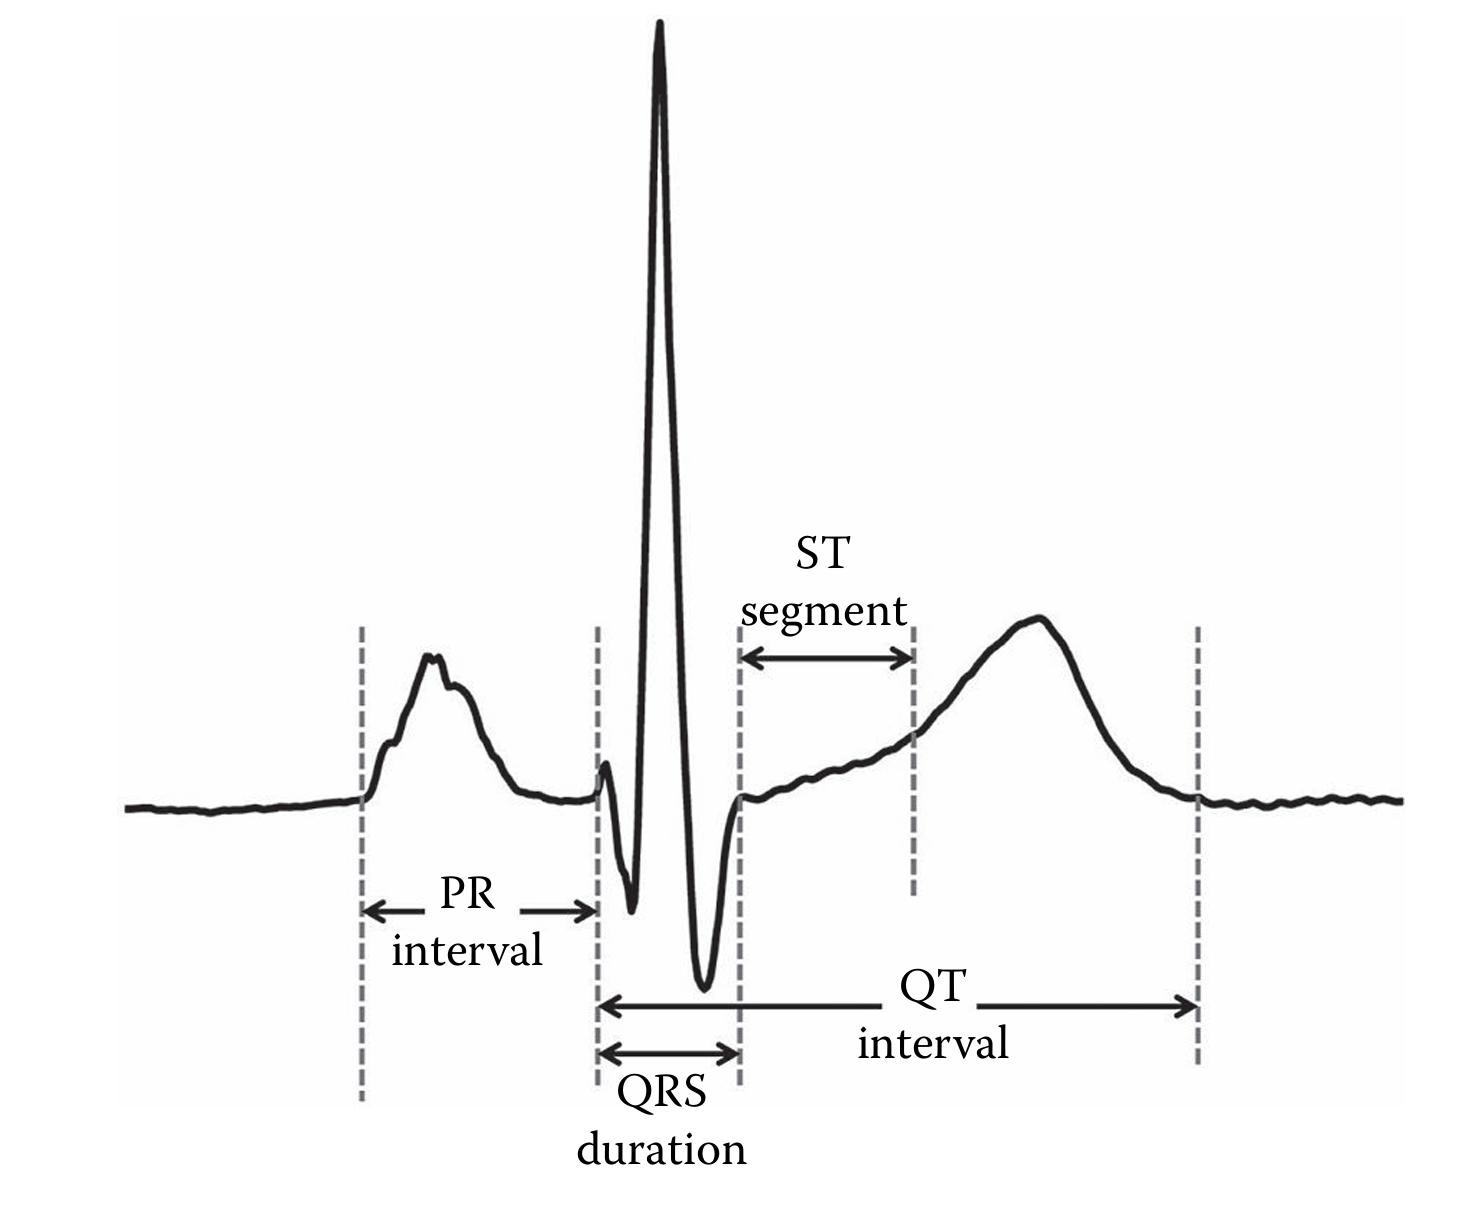
\includegraphics[width=0.6\linewidth]{assets/QRS.png}
    \caption{Ilustração dos intervalos e segmentos padrão medidos no ECG. Fonte: \cite{webster}.}
    % \label{fig:enter-label}
\end{figure}

%colocar figugra

Em condições normais de repouso, o ritmo sinusal apresenta frequência cardíaca entre 60 a 100 bpm (algumas diretrizes admitem entre 50–99 bpm) (\citeay{guyton2021fisiologia}). As medidas temporais padronizadas incluem o \textit{intervalo PR} (do início da onda P ao início do QRS), associado ao tempo de condução AV, com duração típica de 0{,}12--0{,}20~s~ (\citeay{marriott2018practical}). O \textit{intervalo QT} (do início do QRS até o fim da onda T), relacionado à duração da despolarização-repolarização ventricular, geralmente varia entre 0,35 e 0,45 s. O complexo QRS normal é estreito, durando cerca de 0{,}06--0{,}10~s, refletindo condução ventricular rápida pelas vias especializadas. Morfologicamente, a \textit{onda P} tem baixa amplitude ($\leq$0{,}25~mV) e curta duração (<0{,}12~s), enquanto o QRS tem amplitude maior ($\sim$1~mV) e a onda T possui polaridade geralmente concordante com o QRS (\citeay{brazilian_guidelines_ecg}). Esses parâmetros quantificáveis são essenciais para diferenciar padrões normais e patológicos, como bloqueios atrioventriculares, bloqueios de ramo ou prolongamentos de QT com potencial arritmogênico.

A aquisição precisa do sinal \acs{ECG} requer conformidade com especificações técnicas rigorosas, estabelecidas por normas como \textit{ANSI/AAMI EC11}, \textit{IEC 60601-2-25} e \textit{IEC 60601-2-47}. O circuito de entrada deve garantir alta rejeição de modo comum (\textit{CMRR} típico > 90 dB) e tolerância a tensões de offset nos eletrodos de até ±300 mV, já que o sinal útil está na ordem de 1 mV (AAMI, \citeyear{aamiEC11}). A largura de banda depende do propósito: aplicações diagnósticas exigem captura de frequências entre 0{,}05 Hz e 150 Hz, enquanto a monitorização ambulatorial pode operar em bandas entre 0{,}5–40 Hz para reduzir artefatos e interferências(IEC, \citeyear{iec60601}). Após amplificação e filtragem, o sinal é digitalizado com taxas de amostragem típicas entre 250 e 500 Hz, preservando a morfologia do QRS.


Em contextos clínicos, a análise eletrocardiográfica padrão baseia-se no sistema de 12 derivações, que permite a visualização da atividade elétrica cardíaca em múltiplos planos—frontal e horizontal—proporcionando uma avaliação abrangente da condução e da repolarização miocárdica. As derivações bipolares dos membros (DI, DII e DIII) e as unipolares aumentadas (aVR, aVL e aVF) compõem o plano frontal, fornecendo diferentes ângulos de observação da atividade elétrica em direção aos eletrodos dos membros. Já as derivações precordiais (V1 a V6), dispostas na parede torácica, integram o plano horizontal e são fundamentais para localizar alterações segmentares, como na identificação de infartos transmurais e bloqueios de ramo. A correta interpretação dessas 12 derivações exige compreensão da vetorização do impulso elétrico e da anatomia cardíaca, pois cada uma reflete a atividade elétrica de regiões específicas do miocárdio, sendo imprescindível para a caracterização topográfica de eventos isquêmicos, distúrbios de condução e alterações eletrolíticas. Assim, o ECG de 12 canais permanece uma ferramenta diagnóstica insubstituível, sintetizando informações morfológicas, temporais e espaciais do ciclo cardíaco com elevado grau de resolutividade clínica. (\citeay{brazilian_guidelines_ecg}; \citeay{marriott2018practical})





\section{Fundamentos da Tecnologia LoRaWAN}
\label{sec:lorawan}

A tecnologia LoRaWAN posiciona-se entre as redes de longa distância e baixa potência (\textit{Low Power Wide Area Networks} -- LPWAN), categoria concebida para conectar grande número de dispositivos que transmitem pequenos volumes de dados de forma esporádica, com ênfase em alcance e autonomia energética em detrimento da taxa de transferência. Compreender seus fundamentos é essencial para justificar as decisões de projeto adotadas neste trabalho, em especial a escolha da classe de operação e a estratégia de transmissão (Capítulo~\ref{chap:metodologia}).

\subsection{Modulação LoRa}
\label{sec:moduloLora}

Na camada física, o LoRa emprega a modulação por espalhamento espectral do tipo \textit{Chirp Spread Spectrum} (\acs{CSS}), na qual a informação é codificada em sinais cuja frequência varia continuamente ao longo do tempo (\textit{chirps}) (\citeay{loraSpec}). Essa técnica confere elevada robustez a interferências e a efeitos de propagação por múltiplos percursos (\textit{multipath}), além de permitir a recuperação de sinais com potência abaixo do nível de ruído. O principal parâmetro da modulação é o fator de espalhamento (\textit{Spreading Factor} -- SF), que varia tipicamente de 7 a 12: fatores mais altos aumentam o alcance e a sensibilidade do receptor, ao custo de maior tempo de transmissão e menor taxa de dados (\citeay{loraOverview}). Em conjunto com a largura de banda (\textit{Bandwidth} -- BW), geralmente de 125 kHz, o SF determina a taxa de transmissão efetiva e o tempo de ocupação do canal (\textit{Time on Air}).

\subsection{Arquitetura da Rede}
\label{sec:arqLora}

O LoRaWAN define a camada de controle de acesso ao meio (MAC) sobre a modulação LoRa, organizando a comunicação segundo uma topologia em estrela de estrelas (\textit{star-of-stars}). Nessa arquitetura, os dispositivos finais (\textit{end-devices}) comunicam-se por difusão com um ou mais \textit{gateways}, que atuam como pontes transparentes e encaminham os pacotes recebidos a um servidor de rede (\textit{network server}) por meio de uma conexão IP convencional. O servidor de rede é responsável por remover pacotes duplicados, validar a autenticidade dos dispositivos, gerenciar os parâmetros de transmissão e repassar os dados ao servidor de aplicação (\citeay{lorawan1}; \citeay{s23208440}). A segurança é assegurada por criptografia AES de 128 bits em dois níveis independentes — rede e aplicação —, garantindo a confidencialidade dos dados desde o dispositivo até a aplicação final.

\subsection{Classes de Operação}
\label{sec:classesLora}

A especificação LoRaWAN define três classes de operação, que estabelecem o compromisso entre latência de comunicação no sentido descendente (\textit{downlink}) e consumo de energia, conforme resume a Tabela~\ref{tab:classesLora} (\citeay{loraOverview}; \citeay{lorawan1}).

\begin{table}[h]
    \centering
    \caption{Classes de operação do protocolo LoRaWAN.}
    \begin{tabular}{l|>{\arraybackslash}m{6.5cm}|c}
        \textbf{Classe} & \textbf{Funcionamento} & \textbf{Consumo} \\ \hline
        A & Duas janelas curtas de recepção abertas somente após cada \textit{uplink}; \textit{downlink} apenas em resposta. & Mínimo \\ \hline
        B & Janelas de recepção adicionais, agendadas por \textit{beacons} sincronizados do \textit{gateway}. & Intermediário \\ \hline
        C & Janela de recepção continuamente aberta, exceto durante a transmissão; menor latência de \textit{downlink}. & Máximo \\ \hline
    \end{tabular}
    \label{tab:classesLora}
\end{table}

A Classe~A é o modo obrigatório, suportado por todos os dispositivos, e o de menor consumo energético, sendo adequado a dispositivos alimentados por bateria. Sua principal limitação reside no fato de que a recepção de mensagens descendentes só ocorre após uma transmissão ascendente, o que restringe a taxa efetiva de comunicação — característica determinante para o comportamento observado nos experimentos deste trabalho (Capítulo~\ref{chap:resultados}).

\subsection{Parâmetros de Transmissão e Limitações}
\label{sec:paramsLora}

A combinação de SF e largura de banda é abstraída em um índice de taxa de dados (\textit{Data Rate} -- DR), cuja correspondência varia conforme o plano regional de frequências. O LoRaWAN opera em bandas de frequência não licenciadas (\textit{Industrial, Scientific and Medical} -- ISM), específicas de cada região: 868 MHz na Europa, 915 MHz nas Américas — incluindo o plano AU915, adotado neste trabalho — e 433 MHz em partes da Ásia (\citeay{s23208440}). O tamanho máximo do \textit{payload} é condicionado ao DR e situa-se na faixa de poucas dezenas a poucas centenas de bytes.

A principal restrição à transmissão frequente decorre das regras de \textit{duty cycle} impostas às bandas ISM, que limitam a fração de tempo em que um dispositivo pode ocupar o canal, obrigando intervalos mínimos entre transmissões. Mecanismos como a taxa de dados adaptativa (\textit{Adaptive Data Rate} -- ADR) permitem ao servidor de rede ajustar dinamicamente o SF e a potência de transmissão de cada dispositivo, otimizando o consumo e a capacidade da rede (\citeay{performanceLoRa}). Tais limitações tornam o LoRaWAN inadequado à transmissão contínua de formas de onda de alta resolução, como o \acs{ECG} amostrado, porém plenamente eficiente para o envio de dados esparsos e de pequeno volume, como parâmetros vitais e alertas de detecção (\citeay{lorawanWaveform}; \citeay{3-lead}) — premissa que fundamenta a abordagem de processamento na borda adotada neste trabalho.




\chapter{Metodologia}
\label{chap:metodologia}

O desenvolvimento deste trabalho foi organizado em quatro frentes complementares, integradas em um único fluxo de dados que vai da aquisição do biopotencial até o monitoramento clínico: (i) um dispositivo embarcado responsável pela captura do sinal de \acs{ECG}, pelo seu processamento na borda e pela transmissão do resumo de cada segmento analisado; (ii) a infraestrutura de rede \textit{LoRaWAN}, composta por um \textit{gateway} e por um servidor de rede local; (iii) um serviço de ingestão que recebe os resumos da rede, classifica-os e os persiste em nuvem como eventos cardíacos; e (iv) um aplicativo móvel que apresenta esses eventos aos profissionais de saúde em tempo real, sinalizando como eventos de alerta aqueles de maior gravidade clínica.

Diferentemente das abordagens que transmitem a forma de onda completa do \acs{ECG}, este trabalho adotou a estratégia de \textit{processamento na borda} (\textit{edge computing}): a detecção de eventos cardíacos foi realizada no próprio dispositivo embarcado, e apenas um resumo compacto de cada segmento analisado foi transmitido pela rede \textit{LoRaWAN}. Essa decisão, detalhada na Seção~\ref{sec:transmissaoLora}, contornou as restrições de \textit{duty cycle} e de taxa de dados inerentes ao protocolo, viabilizando o monitoramento contínuo em uma rede de longo alcance e baixo consumo.

A Figura~\ref{fig:topologia} apresenta a arquitetura completa do sistema. O sinal foi captado por eletrodos conectados ao paciente, digitalizado, processado e transmitido por um sistema embarcado portátil, montado experimentalmente. O \textit{gateway} \textit{LoRaWAN} encaminhou os pacotes ao servidor de rede \textit{ChirpStack}, que os publicou em um \textit{broker} \acs{MQTT}. Um serviço de ingestão consumiu essas mensagens e gravou os eventos no banco de dados em nuvem (\textit{Firestore}), de onde o aplicativo móvel os leu em tempo real.

\begin{figure}[ht]
    \centering
    \resizebox{\linewidth}{!}{%
    \begin{tikzpicture}[
        >={Stealth[round]},
        box/.style={draw, rounded corners, align=center, minimum height=1.05cm, minimum width=2.1cm, font=\footnotesize},
        elet/.style={draw, line width=0.9pt, circle, minimum size=0.42cm, inner sep=0pt},
        lbl/.style={font=\scriptsize, align=center},
        node distance=0.9cm and 1.6cm
    ]
        % Eletrodos: três anéis empilhados verticalmente
        \node[elet] (e1) {};
        \node[elet, below=0.18cm of e1] (e2) {};
        \node[elet, below=0.18cm of e2] (e3) {};
        \foreach \n in {e1,e2,e3} { \fill (\n.center) circle (0.055); }
        \node[lbl, below=0.20cm of e3] {Eletrodos\\\acs{ECG}};

        \node[box, right=2.1cm of e2, minimum width=4.4cm, text width=4.2cm] (disp)
             {Dispositivo de aquisição e\\processamento do \acs{ECG}\\(detecção na borda)};
        \node[box, right=of disp] (gw)  {\textit{Gateway} +\\ \textit{ChirpStack}};
        \node[box, right=of gw]   (ing) {Ingestor\\(\acs{MQTT})};
        \node[box, right=of ing]  (fs)  {\textit{Firestore}\\(nuvem)};
        \node[box, below=1.0cm of fs] (app) {Aplicativo\\móvel};

        \draw[->] (e1.east) -- (disp.west);
        \draw[->] (e2.east) -- (disp.west);
        \draw[->] (e3.east) -- (disp.west);
        \draw[->] (disp) -- (gw)  node[midway, above, lbl]{\textit{LoRaWAN}};
        \draw[->] (gw)   -- (ing) node[midway, above, lbl]{\acs{MQTT}};
        \draw[->] (ing)  -- (fs);
        \draw[<->] (fs)  -- (app) node[midway, right, lbl]{\acs{SDK}};
    \end{tikzpicture}%
    }
    \caption{Topologia geral do sistema de monitoramento, da aquisição do sinal de \acs{ECG} à visualização no aplicativo móvel. A detecção ocorre no dispositivo embarcado, e apenas o resumo de cada segmento trafega pela rede.}
    \label{fig:topologia}
\end{figure}


\section{Dispositivo de Aquisição e Processamento do Sinal de ECG}
\label{sec:dispositivo}

Para a aquisição do ECG e transmissão dos eventos de alerta foram utilizados módulos comerciais de baixo custo, selecionados com o objetivo de obter um sistema compacto, confiável e energeticamente eficiente, adequado a aplicações de telemedicina e monitoramento remoto. A escolha dos componentes priorizou a alta resolução na aquisição do biopotencial, a capacidade de comunicação de longo alcance e a disponibilidade de recursos de processamento embarcado.

\subsection{Seleção dos Componentes de Hardware}
\label{sec:selecaoHardware}

A definição do microcontrolador considerou capacidade de processamento, conectividade, consumo energético, dimensões e custo. Optou-se pelo módulo XIAO ESP32-S3, que reúne, em um encapsulamento de dimensões reduzidas (21~$\times$~17,5~mm), um processador de dois núcleos, suporte nativo a \textit{Wi-Fi} e \textit{Bluetooth}, controlador de recarga de bateria (íons de lítio) integrado e memória \textit{PSRAM} de 8~MB. Esse último recurso foi determinante para o projeto, pois permitiu armazenar em memória os segmentos de 30~s de sinal necessários ao algoritmo de detecção. A Tabela~\ref{tab:mcu} compara o módulo escolhido com o Arduino~Uno, plataforma recorrente em trabalhos correlatos.

\begin{table}[h]
    \centering
    \caption{Comparativo entre os microcontroladores avaliados.}
    \begin{tabular}{l|>{\centering\arraybackslash}m{3.2cm}|>{\centering\arraybackslash}m{3.2cm}}
         & \textbf{XIAO ESP32-S3} & \textbf{Arduino Uno} \\ \hline
        \textbf{Núcleo} & \textit{Xtensa} LX7 \mbox{dual-core} 32 bits & ATmega328P 8 bits \\ \hline
        \textbf{Frequência} & até 240 MHz & 16 MHz \\ \hline
        \textbf{Memória} & 512 KB SRAM + 8 MB PSRAM & 2 KB SRAM \\ \hline
        \textbf{Conectividade} & \textit{Wi-Fi} + \textit{Bluetooth}/BLE & nenhuma nativa \\ \hline
        \textbf{Bateria} & controlador de carga integrado & externo \\ \hline
        \textbf{Dimensões} & 21 $\times$ 17,5 mm & 68,6 $\times$ 53,4 mm \\ \hline
        \textbf{Preço aproximado \acs{FOB}} & USD 9,90 & USD 11,90 \\ \hline
    \end{tabular}
    \label{tab:mcu}
\end{table}

Para a aquisição do sinal de ECG, a revisão bibliográfica evidenciou que a maioria dos trabalhos emprega o módulo AD8232. Esse componente, contudo, apresenta limitações relevantes: não dispõe de conversor analógico-digital (A/D) integrado, exigindo o uso do \acs{ADC} interno do microcontrolador, cuja resolução efetiva (10--12 bits) e taxa de amostragem são limitadas; além disso, oferece uma única derivação \citep{AnalogDevices_AD8232}. Optou-se, portanto, pelo módulo CJMCU-1293, baseado no \acs{AFE} ADS1293, que integra três canais simultâneos, conversão de 24~bits e taxa de amostragem programável \citep{TexasInstruments_ADS1293}. A Tabela~\ref{tab:ads_vs_ad8232} sintetiza as vantagens do módulo adotado.

\begin{table}[h]
    \centering
    \caption{Comparativo entre os \acs{AFE} ADS1293 e AD8232 para aplicações em \acs{ECG}.}
    \begin{tabular}{l|>{\centering\arraybackslash}m{4.5cm}|>{\centering\arraybackslash}m{4.5cm}}
         & \textbf{ADS1293 (CJMCU-1293)} & \textbf{AD8232} \\ \hline
        \textbf{Conversor A/D} & 24 bits & Não possui (saída analógica) \\ \hline
        \textbf{Canais} & Até 3 canais simultâneos & 1 canal \\ \hline
        \textbf{Taxa de amostragem} & Programável (até 25,6 kSPS) & Definida pelo microcontrolador externo \\ \hline
        \textbf{Resolução efetiva} & 24 bits nativos & 10--12 bits (ADC do MCU) \\ \hline
        \textbf{Consumo de energia} & 0,3 mW por canal & Muito baixo (depende do circuito externo) \\ \hline
        \textbf{Recursos para ECG} & RLD, detecção de eletrodo solto, filtros programáveis & RLD, detecção de eletrodo solto \\ \hline
        \textbf{Aplicação típica} & ECG portátil de alta precisão; pesquisa biomédica & Ensino, prototipagem, \textit{wearables} simples \\ \hline
    \end{tabular}
    \label{tab:ads_vs_ad8232}
\end{table}

A transmissão dos dados coube ao módulo \textit{LoRa} Wio-SX1262, escolhido pela comunicação de longo alcance e pelo baixo consumo característicos da tecnologia. A alimentação do conjunto foi provida por uma bateria de íons de lítio de 3,7~V. 

\subsection{Arquitetura e Funcionamento do Dispositivo}
\label{sec:arqDispositivo}

O ADS1293 registra os sinais bioelétricos do coração e os transfere já digitalizados ao microcontrolador por meio de um barramento \acs{SPI} (\textit{Serial Peripheral Interface}). A Tabela~\ref{tab:pinagem} apresenta a pinagem utilizada na interligação entre o ADS1293 e o XIAO ESP32-S3. O sinal de interrupção \acs{DRDY} (\textit{Data Ready}) foi empregado para sinalizar, a cada nova amostra disponível, a leitura pelo microcontrolador, garantindo a aquisição em taxa constante.

\begin{table}[h]
    \centering
    \caption{Pinagem da interface \acs{SPI} entre o ADS1293 e o XIAO ESP32-S3.}
    \begin{tabular}{l|c|l}
        \textbf{Sinal} & \textbf{Pino XIAO} & \textbf{Função} \\ \hline
        DRDY & D1 & Interrupção: amostra pronta \\ \hline
        CS   & D3 & \textit{Chip Select} \\ \hline
        SCK  & D8 & \textit{Clock} \acs{SPI} \\ \hline
        MISO & D9 & \textit{Master In, Slave Out} \\ \hline
        MOSI & D10 & \textit{Master Out, Slave In} \\ \hline
    \end{tabular}
    \label{tab:pinagem}
\end{table}

A Figura~\ref{fig:conexoes} mostra a interligação completa entre os módulos. A comunicação com o ADS1293 emprega sete conexões: cinco de natureza digital e duas de alimentação. As linhas digitais compreendem o barramento \acs{SPI} propriamente dito — \textit{clock} (SCK), dados do microcontrolador para o \acs{AFE} (MOSI, ligado ao pino SDI do módulo), dados do \acs{AFE} para o microcontrolador (MISO, ligado ao pino SDO) e seleção de dispositivo (CS, ligado ao pino CSB) — acrescidas do sinal de interrupção \acs{DRDY} (pino DRDYB), que sinaliza cada nova amostra disponível. As duas conexões restantes são a alimentação de 3,3~V e o GND.

Quanto à energia, o conjunto é alimentado por uma bateria de íons de lítio de 3,7~V, modelo 18650 (18~mm de diâmetro por 65~mm de comprimento) conectada diretamente aos terminais de bateria (BAT) do XIAO ESP32-S3; o regulador interno do microcontrolador disponibiliza os 3,3~V que alimentam o ADS1293, respeitando o limite de tensão analógica (\textit{AVDD}) de 3,6~V do componente. A porta USB-C destina-se exclusivamente à recarga da bateria, não alimentando o circuito durante a operação. O módulo \textit{LoRa} Wio-SX1262, por sua vez, ocupa um barramento \acs{SPI} dedicado, com pinos internos distintos, o que elimina conflito de comunicação com o \acs{AFE}.

\begin{figure}[htb]
\centering
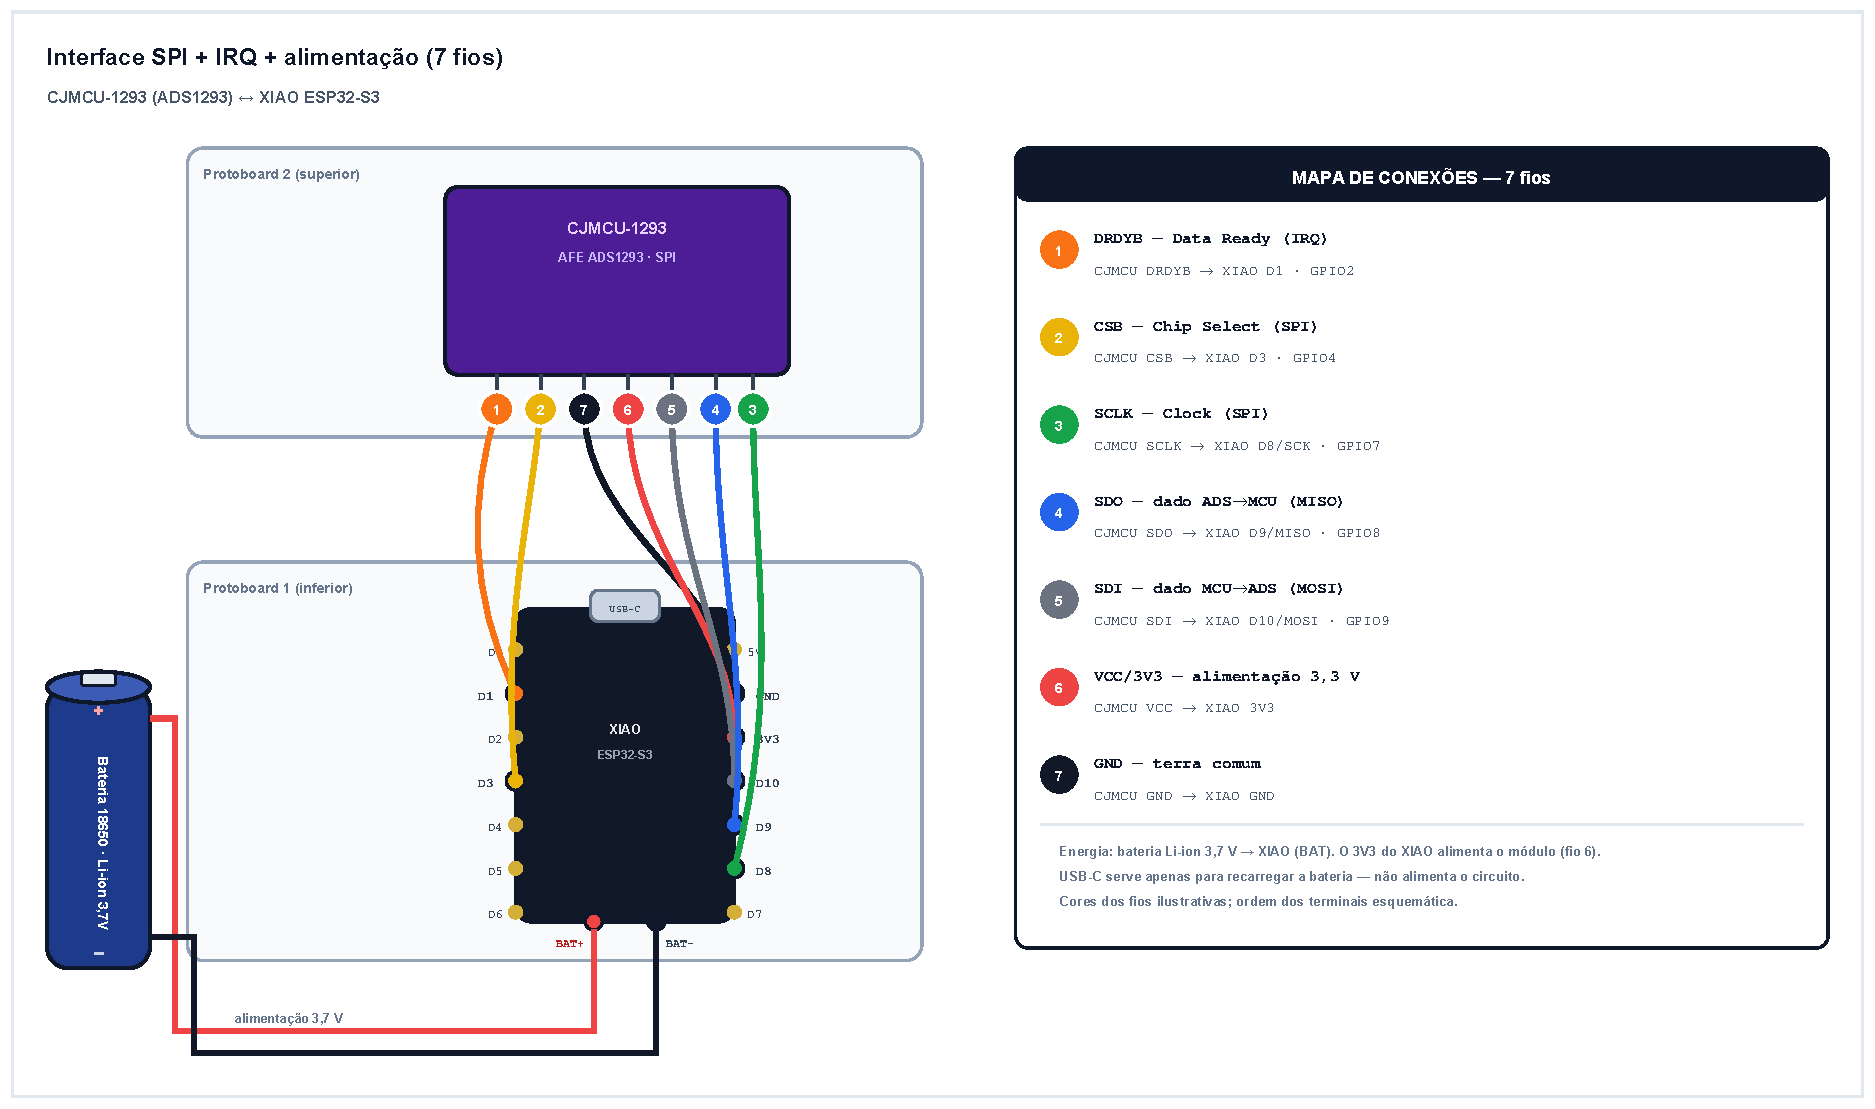
\includegraphics[width=0.95\textwidth]{assets/diagrama_conexoes.pdf}
\caption{Diagrama de conexões do protótipo: interface \acs{SPI} e interrupção entre o \acs{AFE} CJMCU-1293 (ADS1293) e o XIAO ESP32-S3, alimentação a partir da bateria de íons de lítio e recarga por USB-C. As cores dos condutores são ilustrativas.}
\label{fig:conexoes}
\end{figure}

A aquisição foi realizada segundo o triângulo de \textit{Einthoven}, obtendo-se três derivações a partir dos 3 eletrodos fixados no tórax. As derivações I e II foram medidas diretamente pelos canais 1 e 2 do ADS1293, e a derivação III foi calculada por meio da lei de \textit{Einthoven}, conforme as Equações~\ref{eq:leadI} a~\ref{eq:leadIII}:

\begin{align}
    \text{Derivação I}   &= \text{LA} - \text{RA} \label{eq:leadI} \\
    \text{Derivação II}  &= \text{LL} - \text{RA} \label{eq:leadII} \\
    \text{Derivação III} &= \text{Derivação II} - \text{Derivação I} \label{eq:leadIII}
\end{align}

\noindent em que RA, LA e LL representam, respectivamente, os eletrodos do braço direito, do braço esquerdo e da perna esquerda. A derivação II foi adotada como referência para o algoritmo de detecção, por apresentar, tipicamente, a maior amplitude do complexo QRS. A Figura~\ref{fig:diagrama_ecg} ilustra o diagrama de blocos do dispositivo.

\begin{figure}[ht]
    \centering
    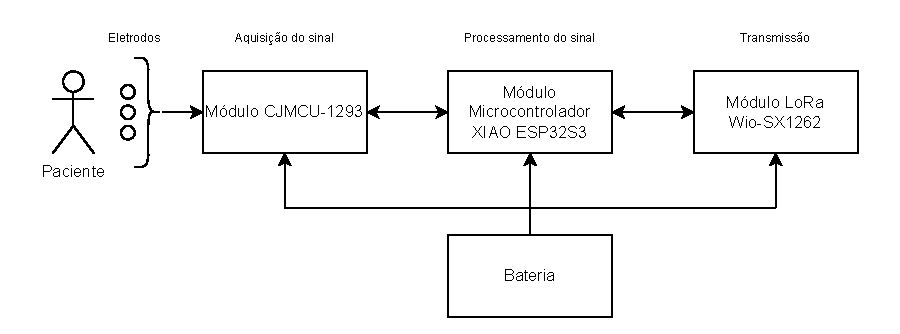
\includegraphics[width=1\linewidth]{assets/blocosDispositivoHardware.drawio.pdf}
    \caption{Diagrama de blocos do dispositivo de aquisição e transmissão do sinal de \acs{ECG}.}
    \label{fig:diagrama_ecg}
\end{figure}


\subsection{Módulo de Comunicação Wio-SX1262}
\label{sec:sx1262}

O Wio-SX1262 é um módulo \textit{LoRa} baseado no transceptor \textit{Semtech} SX1262, projetado para transmissões de longo alcance e baixo consumo. Suas principais características, conforme o fabricante \citep{WioSX1262Datasheet}, são:

\begin{itemize}
    \item \textbf{Consumo em repouso}: 1,62 µA em modo \textit{sleep}.
    \item \textbf{Frequência de operação}: 862--930 MHz, abrangendo as principais regulamentações regionais do \textit{LoRaWAN}.
    \item \textbf{Potência de transmissão}: até 22 dBm (158 mW).
    \item \textbf{Sensibilidade de recepção}: até -136,73 dBm (SF12, largura de banda de 125 kHz).
    \item \textbf{Interfaces}: comunicação \acs{SPI} com o microcontrolador e conector \acs{IPEX} para antena externa.
\end{itemize}

No XIAO ESP32-S3, o Wio-SX1262 ocupa um barramento \acs{SPI} dedicado, com pinos internos distintos dos utilizados pelo ADS1293, eliminando conflitos de comunicação entre os dois periféricos.

\subsection{Módulo de Aquisição CJMCU-1293 (ADS1293)}
\label{sec:cjmcu}

O CJMCU-1293 é um módulo de desenvolvimento que integra o \acs{AFE} (\textit{Analog Front End}) ADS1293, circuito integrado de baixo consumo projetado para aplicações médicas portáteis. Suas principais características são:

\begin{itemize}
    \item \textbf{Arquitetura e precisão}: 3 canais de alta resolução para aquisição simultânea de \acs{ECG}; conversão A/D de 24 bits; taxa de amostragem programável de até 25,6 kSPS.
    \item \textbf{Consumo de energia}: 0,3 mW por canal, com modos de baixo consumo e \textit{standby}.
    \item \textbf{Faixa de operação}: alimentação analógica de 2,7 V a 5,5 V e entrada diferencial de ±400 mV, compatível com eletrodos de \acs{ECG} comuns.
    \item \textbf{Funcionalidades para ECG}: detecção de eletrodo desconectado (\textit{Lead-Off Detection}); entradas com imunidade a interferência eletromagnética (\textit{EMI-Hardened Inputs}); e amplificador de perna direita (\textit{Right-Leg Drive} -- RLD), que reduz o ruído de modo comum, em especial a interferência de 60 Hz da rede elétrica.
    \item \textbf{Interface}: comunicação via \acs{SPI} com o microcontrolador.
\end{itemize}

A configuração do ADS1293 foi realizada para operação em três derivações (\textit{3-Lead}), com a detecção de modo comum e o amplificador RLD habilitados, condições necessárias à obtenção de um sinal limpo durante a movimentação do paciente.

Em uma aplicação convencional, o amplificador RLD requer um quarto eletrodo, posicionado na perna direita do paciente, para o qual o sinal de contrarreação de modo comum é aplicado. Com o objetivo de reduzir o número de cabos e simplificar a montagem, optou-se por dispensar esse eletrodo dedicado e adotar uma topologia de \textit{driven-leg} com apenas três eletrodos, na qual as funções de detecção e de contrarreação do modo comum são atribuídas a eletrodos distintos.

A detecção de modo comum, realizada pelo \textit{Common-Mode Detector} do ADS1293, calcula a média das tensões dos pinos de entrada habilitados no registrador \texttt{CMDET\_EN} \citep{TexasInstruments_ADS1293}. Habilitaram-se apenas os pinos IN1 e IN3 (\texttt{CMDET\_EN = 0x05}), correspondentes aos eletrodos do braço direito (RA) e da perna esquerda (LL), deixando o eletrodo do braço esquerdo (LA) livre para receber a contrarreação. O roteamento da saída do RLD, por sua vez, é definido pelos três bits menos significativos (campo \textit{SELRLD}) do registrador \texttt{RLD\_CN}: enquanto o valor padrão da biblioteca de controle (\texttt{SELRLD = 100}) direciona a saída ao pino IN4 (eletrodo de perna direita), o valor adotado neste trabalho (\texttt{SELRLD = 010}) a direciona ao pino IN2, associado ao eletrodo LA. Dessa forma, a média de modo comum é obtida de RA e LL e reinjetada por LA, mantendo-se a separação entre os eletrodos de detecção e de contrarreação característica da topologia clássica de \textit{driven-leg} e obtendo-se a atenuação do ruído de modo comum de 60~Hz com apenas três eletrodos. A taxa de conversão foi definida pelos registradores de decimação \texttt{R2} e \texttt{R3}, programados por meio da configuração \texttt{SPS\_256} da biblioteca de controle, o que resulta na taxa efetiva de 640 amostras por segundo por canal --- valor verificado experimentalmente e adotado em todo o processamento subsequente.


\section{Firmware Embarcado}
\label{sec:firmware}

O \textit{firmware} do dispositivo foi desenvolvido em C++ sobre a plataforma \textit{Arduino}, e estruturado em torno de um laço orientado a interrupção: a cada borda do sinal \acs{DRDY}, uma amostra das três derivações foi lida do ADS1293 acumulada em um \textit{buffer}. Ao completar um segmento de 30~s, o algoritmo de detecção de arritmias foi executado, o resultado foi registrado em memória não volátil e, então, transmitido pela rede \textit{LoRaWAN}.

\subsection{Aquisição e Condicionamento do Sinal}
\label{sec:condicionamento}

As amostras brutas, fornecidas pelo conversor de 24 bits, foram convertidas para a escala de tensão segundo a Equação~13 do manual do componente \citep{TexasInstruments_ADS1293}, $v = \left(raw/\mathrm{ADC_{MAX}} - 1/2\right)\cdot 2V_{ref}/G$, em que $G = 3{,}5$ é o ganho do amplificador de instrumentação, $V_{ref} = 2{,}4$~V é a referência interna e $\mathrm{ADC_{MAX}}$ é o fundo de escala do conversor. Cabe observar que esse fundo de escala não corresponde à excursão total de 24 bits: ele é determinado pelas razões de decimação programadas em \texttt{R2} e \texttt{R3}, valendo $\mathrm{ADC_{MAX}} = \mathtt{0xC35000}$ na configuração adotada, e a saída é codificada em binário com \textit{offset}, de modo que a meia escala corresponde a 0~V diferencial. Em seguida, cada derivação foi submetida a uma cascata de dois filtros digitais de resposta ao impulso infinita (\acs{IIR}): um filtro passa-baixas, com frequência de corte de 40 Hz, para atenuar o ruído muscular e a interferência da rede elétrica; e um filtro passa-altas, com frequência de corte de 0,5 Hz, para remover o desvio de linha de base (\textit{baseline wander}) e a componente contínua de \textit{offset} dos eletrodos. Ambos os filtros são de primeira ordem: o passa-baixas na forma de média móvel exponencial e o passa-altas na forma canônica de um polo, com coeficientes $\alpha \approx 0{,}3247$ e $\alpha \approx 0{,}9951$, respectivamente. Optou-se pela estrutura \acs{IIR}, em detrimento de um filtro \acs{FIR} de fase linear, pelo custo computacional: um \acs{FIR} equivalente, projetado por janelamento de \textit{Hamming}, exigiria da ordem de $3{,}3\,f_s/\Delta f$ coeficientes --- algumas centenas para o corte de 40~Hz e alguns milhares para o de 0,5~Hz ---, contra uma única multiplicação-acumulação e um estado por amostra na estrutura adotada, em um microcontrolador que executa concomitantemente a aquisição, o armazenamento do segmento e a pilha \textit{LoRaWAN}. A distorção de fase decorrente concentra-se abaixo de 2~Hz e afeta sobretudo o segmento ST e a onda T, e não a localização temporal do complexo QRS, da qual dependem as grandezas efetivamente medidas pelo sistema; ademais, o realce do QRS no algoritmo de detecção (Seção~\ref{sec:deteccaoBorda}) é realizado por um filtro janela-sinc, de fase linear. Os coeficientes foram calculados para a taxa de amostragem do sistema, de 640~SPS, decorrente das razões de decimação programadas no conversor (Equação~\ref{eq:odr}) e suficiente, com ampla margem, para a banda de interesse do sinal, limitada a 40~Hz pelo próprio passa-baixas. Cabe registrar que essa taxa não corresponde ao valor nominal sugerido pela nomenclatura da configuração empregada na biblioteca de controle, discrepância identificada durante a caracterização do componente e detalhada no Capítulo~\ref{chap:resultados}.

A saída de depuração pela interface serial foi desacoplada da aquisição, de modo a preservar a integridade temporal do sinal processado. A interface opera a 230.400 bits por segundo e cada amostra impressa ocupa cerca de 42 caracteres, com as três derivações em representação textual; a 640 amostras por segundo, a vazão exigida é de aproximadamente 270~kbit/s, acima da capacidade do enlace. Excedida essa capacidade, a operação de escrita bloqueia o laço principal enquanto o \textit{buffer} de transmissão se esvazia, o que ocasiona a perda de interrupções \acs{DRDY}, introduz descontinuidades no \textit{buffer} de detecção e distorce os intervalos R-R. Para evitá-lo, a saída de depuração foi decimada — apenas uma a cada quatro amostras é enviada à serial, o que reduz a vazão exigida a cerca de 67~kbit/s —, enquanto o \textit{buffer} de detecção continuou a receber todas as amostras. Nas coletas automatizadas, em que apenas as linhas de resumo interessam, a impressão de amostras foi inteiramente desativada. Preservou-se, assim, a visualização em tempo real sem comprometer o sinal efetivamente submetido à detecção.

\subsection{Detecção de Eventos na Borda}
\label{sec:deteccaoBorda}

O núcleo do processamento embarcado consistiu em um algoritmo de detecção de complexos QRS e de classificação de arritmias, aplicado à derivação II de cada segmento de 30~s. Esse algoritmo não é uma contribuição deste trabalho: trata-se do \textit{firmware} de detecção desenvolvido por \citeay{moraesFirmwareECG}, descrito na Seção~\ref{sec:deteccaoEmbarcada}, cujo código-fonte foi cedido pelos autores e aqui reutilizado. 

A adaptação realizada limitou-se ao necessário para a execução na plataforma adotada: ajuste da taxa de amostragem (de 500 para 640~SPS, com a consequente reescrita dos limiares expressos em número de amostras por unidade de tempo), e integração ao \textit{buffer} de aquisição e ao \textit{payload} de transmissão. As regras de decisão dos limiares clínicos passaram por ajustes sutis, de modo a manter a comparabilidade com os resultados originais.

O algoritmo, baseado na análise da derivada do sinal --- método da operação de diferenças (DOM, \textit{Difference Operation Method}) ---, seguiu as etapas:

\begin{enumerate}
    \item \textbf{Diferenciação}: cálculo da diferença discreta entre amostras consecutivas, realçando as transições rápidas associadas ao complexo QRS.
    \item \textbf{Filtragem}: filtragem do sinal diferenciado com um filtro passa-baixas do tipo janela-sinc, suavizando as componentes de alta frequência remanescentes.
    \item \textbf{Limiarização adaptativa}: cálculo de limiares positivo e negativo proporcionais à média das amplitudes de cada polaridade, separando os extremos significativos do ruído de fundo.
    \item \textbf{Pareamento e detecção de picos}: identificação dos pares de extremos (descida e subida) correspondentes a cada complexo QRS e localização dos picos R.
    \item \textbf{Cálculo dos intervalos R-R}: a partir das posições dos picos R, foram obtidos os intervalos R-R e suas estatísticas (média, desvio padrão e diferenças sucessivas), base para a classificação. Essas estatísticas correspondem aos índices de variabilidade da frequência cardíaca no domínio do tempo padronizados por \citeay{hrvTaskForce1996}.
\end{enumerate}


Com base nas estatísticas dos intervalos R-R, o algoritmo classifica o segmento em seis categorias de anormalidade: taquicardia, bradicardia, arritmia sinusal, bloqueio sinoatrial, parada sinoatrial e anomalia não caracterizada. As cinco primeiras provêm do trabalho de \cite{moraesFirmwareECG}; a sexta foi acrescentada neste trabalho e é descrita adiante. A taquicardia é sinalizada quando o intervalo R-R médio é inferior a 600 ms (frequência cardíaca acima de 100 bpm) e a bradicardia quando superior a 1000 ms (abaixo de 60 bpm).

A arritmia sinusal é sinalizada quando a diferença entre dois intervalos R-R consecutivos situa-se entre 120 ms e 80\,\% do intervalo R-R de base. O limite superior não constava da formulação original e foi acrescentado para impedir que a diferença produzida por uma pausa fosse contabilizada também como variabilidade sinusal. Assim, o contador de arritmia passa a representar variações batimento a batimento, enquanto os intervalos longos são avaliados pelos critérios de pausa descritos a seguir.

As duas classes de pausa foram decididas em relação ao ritmo de base do próprio segmento, e não por duração absoluta. No bloqueio sinoatrial de segundo grau, a pausa corresponde a dois ou três intervalos R-R do ritmo de base; na parada sinusal, a pausa excede três intervalos R-R. Adotou-se como ritmo de base a mediana dos intervalos R-R do segmento, por ser menos sensível ao próprio intervalo pausado do que a média. A comparação do bloqueio com os múltiplos de dois e três ciclos admitiu tolerância relativa de 5\,\%, considerando a variabilidade fisiológica e as não idealidades do registro. Não se impôs piso de duração absoluta: a uma frequência cardíaca elevada, uma pausa de dois intervalos R-R é breve em termos absolutos, mas continua sendo, por definição, um bloqueio.

A sexta categoria --- anomalia não caracterizada --- foi acrescentada para cobrir os segmentos em que há evidência de anormalidade no ritmo, mas que não corresponde a nenhuma das cinco alterações detectadas. Sinaliza-se essa categoria quando um intervalo de pelo menos uma vez e meia o R-R de base não satisfaz os critérios de arritmia sinusal, bloqueio ou parada. Na prática, ela cobre a descontinuidade entre as faixas: intervalos longos demais para serem tratados como variabilidade sinusal, mas que não se aproximam de dois ou três ciclos e tampouco excedem três ciclos. Trata-se de uma classe residual; ela não substitui a detecção de bloqueio ou parada quando esses critérios são satisfeitos, nem cria um diagnóstico novo.

A justificativa para acrescentar uma categoria, em vez de estender as faixas dos critérios existentes, é de natureza clínica. Alargar o critério de bloqueio para abranger durações intermediárias faria o sistema indicar alterações falsas (falsos positivos). A categoria adicional indica que há anormalidade e que ela não é caracterizável pelos critérios usados atualmente, conduta apropriada a um monitor de triagem, cuja finalidade é encaminhar o paciente para exames mais detalhados. Quando a máscara de \textit{bits} precisa ser convertida em um único rótulo, a anomalia não caracterizada fica por último na ordem de prioridade, pois só deve aparecer como classificação principal quando nenhuma alteração específica foi detectada.

Registre-se que a formulação relativa das pausas, o teto do critério de arritmia e a categoria adicional foram as adaptações de regra de decisão incorporadas neste trabalho ao algoritmo de \citet{moraesFirmwareECG}. Essas adaptações foram conduzidas sob orientação dos autores do algoritmo, com o objetivo de adequar a classificação ao uso no protótipo desenvolvido e de preservar, no registro transmitido, informações úteis à triagem. Suas consequências experimentais são reportadas na Seção~\ref{sec:resValidacaoFinal}.

O resultado primário da classificação é a máscara de \textit{bits}, de modo que mais de uma alteração pode permanecer registrada no mesmo segmento. Taquicardia, bradicardia, arritmia sinusal, bloqueio, parada e anomalia não caracterizada não são mutuamente excludentes no resumo gravado. A ordem de prioridade é aplicada apenas depois, na etapa de ingestão, quando a máscara precisa ser representada por um único tipo de evento para indexação e apresentação no sistema (Seção~\ref{sec:resPipeline}).

Para evitar resultados indevidos, segmentos com menos de três picos R detectados foram marcados como erro de processamento. Esse limite é operacional: com menos de três picos há, no máximo, um intervalo R-R, quantidade insuficiente para calcular diferenças sucessivas entre intervalos e aplicar os critérios temporais da classificação. Essa condição não equivale à classe normal nem à anomalia não caracterizada. A classe normal corresponde ao segmento com picos suficientes e sem critérios de anormalidade satisfeitos; a anomalia não caracterizada, por sua vez, exige picos suficientes e ao menos um intervalo longo que não se enquadre nas classes nomeadas. A Tabela~\ref{tab:criteriosClassificacao} resume os critérios aplicados a cada segmento.

\begin{table}[H]
    \centering
    \caption{Critérios de classificação aplicados aos intervalos R-R de cada segmento.}
    \label{tab:criteriosClassificacao}
    \small
    \setlength{\tabcolsep}{4pt}
    \renewcommand{\arraystretch}{1.08}
    \begin{tabular}{>{\raggedright\arraybackslash}p{3.6cm}>{\raggedright\arraybackslash}p{5.1cm}>{\raggedright\arraybackslash}p{5.0cm}}
        \hline
        \textbf{Condição} & \textbf{Critério} & \textbf{Observação} \\ \hline
        Erro de processamento & Menos de três picos R detectados & Não há intervalos suficientes para aplicar os critérios temporais; o segmento é mantido apenas no registro local. \\ \hline
        Taquicardia & $\overline{RR} < 600$ ms & Equivale a frequência cardíaca média acima de 100 bpm. \\ \hline
        Bradicardia & $\overline{RR} > 1000$ ms & Equivale a frequência cardíaca média abaixo de 60 bpm. \\ \hline
        Arritmia sinusal & $120$ ms $< |\Delta RR| < 0{,}8\,\widetilde{RR}$ & Conta variações batimento a batimento; o teto evita contabilizar pausas como variabilidade sinusal. \\ \hline
        Bloqueio sinoatrial & $RR_i \approx 2\widetilde{RR}$ ou $RR_i \approx 3\widetilde{RR}$, com tolerância de 5\,\% & Pausa de dois ou três ciclos do ritmo de base. \\ \hline
        Parada sinusal & $RR_i > 3(1+0{,}05)\widetilde{RR}$ & Pausa superior a três ciclos do ritmo de base. \\ \hline
        Anomalia não caracterizada & $RR_i \ge 1{,}5\widetilde{RR}$ sem satisfazer os critérios de arritmia sinusal, bloqueio ou parada & Classe residual para intervalo longo não enquadrado nas classes nomeadas. \\ \hline
    \end{tabular}
\end{table}

\subsection{Armazenamento Local}
\label{sec:armazenamento}

Para conferir robustez ao sistema diante de eventuais falhas de comunicação e permitir a validação posterior dos dados, o \textit{firmware} mantem um registro local em memória \textit{flash}, por meio do sistema de arquivos \textit{LittleFS}. Para cada segmento de 30~s, independentemente de sua classificação, é gravado um resumo compacto de 16 bytes contendo o identificador sequencial do segmento, a frequência cardíaca estimada, o intervalo R-R médio e seu desvio padrão, o número de picos detectados e as anormalidades identificadas. O registro local reúne os mesmos campos do \textit{payload} transmitido (Tabela~\ref{tab:payload}), acrescidos do instante de conclusão do processamento, em 4 bytes, e com o identificador do segmento em 32 bits, e não em 16. Daí a diferença entre os 16 bytes gravados e os 10 transmitidos: a gravação em memória \textit{flash} não consome tempo de ocupação do canal, de modo que não há por que truncar os campos, ao passo que no enlace \textit{LoRaWAN} cada byte acrescenta tempo no ar. Adicionalmente, para os segmentos classificados como anormais, o sinal bruto da derivação II foi armazenado integralmente, possibilitando a inspeção \textit{a posteriori} da forma de onda associada ao evento. Foram implementadas políticas de rotação que descartam os registros mais antigos quando o espaço disponível na memória \textit{flash} se aproxima do limite reservado ao armazenamento local, garantindo a operação contínua do dispositivo sem interrupção por falta de espaço.

\subsection{Transmissão via LoRaWAN}
\label{sec:transmissaoFirmware}
\label{sec:transmissaoLora}

A transmissão empregou a biblioteca \textit{RadioLib} (versão 7.1.2) e o protocolo \textit{LoRaWAN} na região AU915 (sub-banda 2), com ativação por \acs{OTAA} (\textit{Over-the-Air Activation}) e operação em Classe~A. Ao final de cada segmento de 30~s do sinal de \acs{ECG}, foi enviado, na porta de aplicação 2, um \textit{payload} de 10 bytes contendo o resumo transmitido do segmento, codificado em formato \textit{big-endian}, conforme a Tabela~\ref{tab:payload}. Esse \textit{payload} é menor que o registro local de 16 bytes porque omite o instante de processamento gravado na memória \textit{flash} e transmite apenas os 16 bits menos significativos do identificador sequencial do segmento. O reduzido tamanho do \textit{payload} foi resultado direto da estratégia de detecção na borda e constituiu o elemento central que viabilizou a transmissão sobre \textit{LoRaWAN}.

Um aspecto prático da ativação por \acs{OTAA} exigiu tratamento específico. A cada reinicialização do dispositivo, o contador de segurança do protocolo de ingresso (\textit{DevNonce}) é reiniciado; como o servidor de rede rejeita valores de \textit{DevNonce} já utilizados, para prevenir ataques de repetição, cada reinício resultava na recusa do ingresso até a limpeza manual dos \textit{nonces} no \textit{ChirpStack}. Para eliminar essa dependência de intervenção, o estado do enlace foi persistido na memória não volátil do microcontrolador (\textit{Non-Volatile Storage} -- NVS, do ESP32): tanto os \textit{nonces} de ingresso quanto o contexto da sessão (chaves derivadas e contadores de quadro) são gravados após cada ativação bem-sucedida e a cada \textit{uplink}. Na inicialização, esse estado é restaurado antes da ativação, o que permite ao dispositivo retomar a sessão existente sem repetir o procedimento de ingresso ou, quando um novo ingresso é necessário, apresentar um \textit{DevNonce} sempre crescente. Dessa forma, o dispositivo tolera reinícios e quedas de energia sem intervenção no servidor de rede, requisito essencial para operação autônoma prolongada.

\begin{table}[h]
    \centering
    \caption{Estrutura do \textit{payload} de 10 bytes transmitido via \textit{LoRaWAN}.}
    \begin{tabular}{c|l|c}
        \textbf{Byte(s)} & \textbf{Campo} & \textbf{Tipo} \\ \hline
        0 & \textit{Flags} de detecção (\textit{bitmask}) & uint8 \\ \hline
        1--2 & Frequência cardíaca (bpm) & uint16 \\ \hline
        3--4 & Intervalo R-R médio (ms) & uint16 \\ \hline
        5--6 & Desvio padrão do R-R (ms) & uint16 \\ \hline
        7 & Número de picos R & uint8 \\ \hline
        8--9 & Identificador do segmento & uint16 \\ \hline
    \end{tabular}
    \label{tab:payload}
\end{table}

O campo de desvio padrão do R-R corresponde ao índice \acs{SDNN} --- desvio padrão dos intervalos entre batimentos --- tal como definido por \citeay{hrvTaskForce1996}, calculado, neste trabalho, sobre a janela de 30~s de cada segmento. Cabe registrar que essa janela é inferior aos 5~min mínimos preconizados naquele documento para os registros curtos, e que os batimentos ectópicos não são excluídos da série antes do cálculo; o valor transmitido presta-se, portanto, à caracterização da dispersão dos intervalos dentro do segmento, e não à comparação direta com os índices de variabilidade reportados na literatura clínica.


O campo de \textit{flags} codificou, em uma máscara de bits, as seis categorias de anormalidade, permitindo o registro de detecções simultâneas em um mesmo segmento. O identificador sequencial do segmento possibilitou ao servidor detectar eventuais perdas de pacotes. A aquisição do \acs{ECG} foi mantida independentemente do sucesso da conexão \textit{LoRaWAN}: na ausência de rede, os dados permaneceram armazenados localmente até a recuperação da comunicação.

A transmissão da forma de onda completa não foi adotada devido às limitações de taxa de dados e de \textit{duty cycle} do \textit{LoRaWAN}, apontadas na literatura para aplicações com \acs{ECG} \citep{lorawanWaveform, 3-lead}. Um segmento de 30~s amostrado a 640~SPS, com 2 bytes por amostra, exigiria 38.400 bytes por derivação, volume incompatível com o envio contínuo em uma rede de baixo consumo. A alternativa de fragmentar e comprimir a forma de onda em múltiplos pacotes foi avaliada preliminarmente, mas a operação em Classe~A impôs intervalos de vários segundos entre transmissões, tornando o fluxo inadequado para monitoramento contínuo.

A solução adotada foi deslocar o processamento para o dispositivo embarcado: em vez de transmitir o traçado, o sistema executou localmente a detecção de arritmias (Seção~\ref{sec:deteccaoBorda}) e enviou apenas o resumo de 10 bytes de cada segmento. Essa estratégia é consistente com estudos que consideram o \textit{LoRaWAN} adequado ao envio de alertas e parâmetros vitais compactos, mas não à transmissão contínua da forma de onda \citep{lorawanWaveform, ecgCompressionLora}. Como contrapartida, a forma de onda completa dos segmentos anormais permaneceu armazenada localmente (Seção~\ref{sec:armazenamento}), disponível para posterior recuperação e análise detalhada, sem onerar o canal de comunicação.


\section{Infraestrutura de Rede LoRaWAN}
\label{sec:infraLora}

A infraestrutura de rede teve por função receber os pacotes transmitidos pelo dispositivo e disponibilizá-los para a aplicação. Ela foi composta por um \textit{gateway} \textit{LoRaWAN} e por um servidor de rede executado localmente, conferindo ao sistema autonomia em relação a redes públicas.

\subsection{Minicomputador Raspberry Pi 3}
\label{sec:rpi3}

O \textit{Raspberry Pi 3} é um computador de placa única (\textit{Single Board Computer} -- \acs{SBC}) baseado em processador \textit{Quad-core ARM Cortex-A53} de 64 bits, com 1 GB de memória \textit{LPDDR2}, conectividade \textit{Wi-Fi}, \textit{Bluetooth} e \textit{Ethernet}, e 40 pinos \acs{GPIO}. No projeto, ele serviu de base computacional para o \textit{gateway}, hospedando tanto o módulo concentrador \textit{LoRa} quanto o servidor de rede \textit{ChirpStack}, e provendo a conexão \textit{Ethernet} de saída para a internet.

\subsection{Módulo Radioenge LoRaWAN Gateway}
\label{sec:radioenge}

O \textit{LoRaWAN Gateway} da \textit{Radioenge} é um módulo concentrador de longo alcance, fornecido no formato de \textit{shield} para acoplamento direto ao \textit{Raspberry Pi 3}. Suas principais características são:

\begin{itemize}
    \item \textbf{Frequência de operação}: 902--928 MHz, em modo \textit{Half-Duplex} (TDD).
    \item \textbf{Modulação e protocolo}: \textit{LoRa/CSS} (\textit{Chirp Spread Spectrum}), compatível com o protocolo \textit{LoRaWAN}.
    \item \textbf{Capacidade de recepção}: até 8 canais simultâneos na banda \textit{LoRaWAN}.
    \item \textbf{Potência de transmissão}: até +27 dBm (0,5 W).
    \item \textbf{Sensibilidade de recepção}: até -137 dBm.
    \item \textbf{Alimentação e consumo}: 5 V \acs{DC}; 300 mA em recepção e 700 mA em transmissão.
\end{itemize}

A Figura~\ref{fig:diagrama_getway} apresenta o diagrama de blocos do \textit{gateway}.

\begin{figure}[ht]
    \centering
    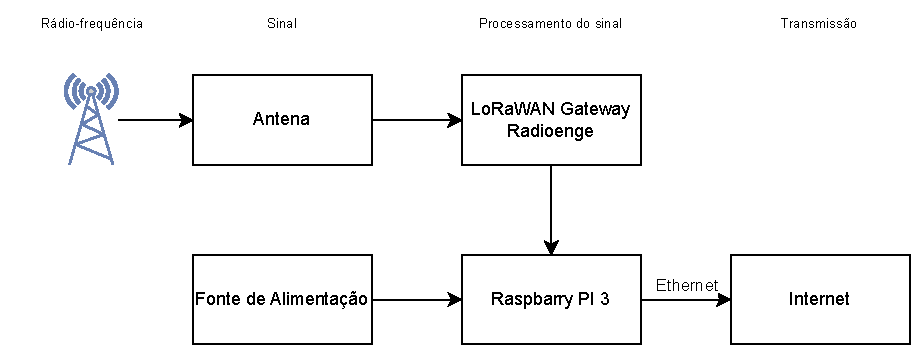
\includegraphics[width=1\linewidth]{assets/diagramaDeBlocoGateway.pdf}
    \caption{Diagrama de blocos do \textit{gateway LoRaWAN}.}
    \label{fig:diagrama_getway}
\end{figure}

\subsection{Servidor de Rede ChirpStack}
\label{sec:chirpstack}

Sobre o \textit{Raspberry Pi 3} foi instalado o \textit{ChirpStack}, servidor de rede \textit{LoRaWAN} de código aberto, responsável por autenticar os dispositivos, desduplicar os pacotes recebidos pelos \textit{gateways} e decodificar o \textit{payload}. Para tanto, configurou-se um decodificador (\textit{codec}) em \textit{JavaScript} que converte os 10 bytes recebidos no objeto estruturado descrito na Tabela~\ref{tab:payload}. Essa função, apresentada na Figura~\ref{fig:decoder}, valida o comprimento do quadro, expande a máscara de bits em indicadores por anomalia e remonta os inteiros de 16 bits a partir dos pares de bytes, disponibilizando o resultado no objeto \texttt{data.object}. Após a decodificação, o \textit{ChirpStack} publica cada evento de \textit{uplink} em um \textit{broker} \acs{MQTT} (\textit{Message Queuing Telemetry Transport}), tornando os dados disponíveis para consumo pela camada de aplicação. A adoção de um servidor de rede local, em vez de uma rede pública, garantiu controle total sobre o roteamento dos dados e maior previsibilidade na comunicação, requisitos importantes em uma aplicação clínica.

\begin{figure}[ht]
\centering
\begin{Verbatim}[fontsize=\small, frame=single]
function decodeUplink(input) {
  var b = input.bytes;
  if (!b || b.length < 10) return { errors: ["payload curto"] };
  var flags = b[0];
  return { data: {
    flags: flags,
    taqui:    (flags & 0x01) !== 0,
    bradi:    (flags & 0x02) !== 0,
    arritmia: (flags & 0x04) !== 0,
    bloqueio: (flags & 0x08) !== 0,
    parada:   (flags & 0x10) !== 0,
    bpm:       (b[1] << 8) | b[2],
    rrMed:     (b[3] << 8) | b[4],
    rrDp:      (b[5] << 8) | b[6],
    numPicos:   b[7],
    segmentId: (b[8] << 8) | b[9]
  }};
}
\end{Verbatim}
\caption{Função decodificadora (\textit{codec}) cadastrada no \textit{ChirpStack}, que converte o \textit{payload} de 10 bytes no objeto consumido pelo serviço de ingestão.}
\label{fig:decoder}
\end{figure}


\section{Ingestão e Persistência dos Dados}
\label{sec:ingestao}

A integração entre a infraestrutura \textit{LoRaWAN} e a aplicação foi realizada por um serviço de ingestão desenvolvido em \textit{Python}. Optou-se por uma arquitetura sem servidor de aplicação dedicado (\textit{serverless}): o único processo de retaguarda em execução contínua foi o ingestor, enquanto a persistência e a leitura dos dados ficaram a cargo de uma plataforma gerenciada em nuvem.

\subsection{Ingestor MQTT}
\label{sec:ingestor}

O ingestor inscreveu no \textit{broker} \acs{MQTT} do \textit{ChirpStack} e, a cada mensagem de \textit{uplink}, executa: a identificação do dispositivo de origem pelo seu \textit{DevEUI}; a verificação do paciente a ele vinculado; a determinação do tipo de evento de maior prioridade clínica a partir da máscara de \textit{flags}; e a gravação do evento cardíaco no banco de dados. Quando o evento é classificado como crítico, o ingestor registra também os eventos de alerta destinados aos profissionais de saúde ativos da respectiva instituição. Para conter o custo de operação da plataforma em nuvem, o serviço foi parametrizado de modo a permitir, opcionalmente, o descarte dos segmentos normais e a restrição das notificações apenas aos eventos críticos.

\subsection{Banco de Dados e Modelo de Dados}
\label{sec:bancoDados}

A persistência foi realizada no \textit{Cloud Firestore}, banco de dados de documentos (\acs{NoSQL}) da plataforma \textit{Firebase}, escolhido por oferecer sincronização em tempo real com os clientes, escalabilidade gerenciada e integração nativa com o serviço de autenticação. Por se tratar de um banco orientado a documentos, o modelo não é relacional: os dados foram organizados em coleções de documentos que se referenciam por meio de identificadores, adotando-se um modelo multi-instituição (\textit{multi-tenant}) em que cada documento referencia a entidade (instituição) à qual pertence. A Tabela~\ref{tab:colecoes} descreve as coleções e seus principais campos, e a Figura~\ref{fig:modeloFirestore} ilustra as referências entre elas.

\begin{table}[h]
    \centering
    \caption{Modelo de dados do \textit{Firestore}: coleções, principais campos e referências.}
    \small
    \begin{tabular}{l|>{\arraybackslash}m{6.7cm}|>{\arraybackslash}m{3.1cm}}
        \textbf{Coleção} & \textbf{Principais campos} & \textbf{Referências} \\ \hline
        \textit{entidades} & id, nome, ativo, criadoEm & --- \\ \hline
        \textit{usuarios} & id, nome, email, perfil, entidadeId, status, criadoEm & entidadeId $\rightarrow$ entidades \\ \hline
        \textit{pacientes} & id, nome, cpf, dataNascimento, ativo, entidadeId, criadoEm & entidadeId $\rightarrow$ entidades \\ \hline
        \textit{dispositivos} & id, devEui, entidadeId, pacienteId, cadastradoPor, criadoEm & entidadeId $\rightarrow$ entidades; pacienteId $\rightarrow$ pacientes \\ \hline
        \textit{eventosCardiacos} & id, dispositivoId, pacienteId, entidadeId, bpm, flags, tipoEvento, rrMed, rrDp, numPicos, segmentId, sinalCritico, origem, criadoEm & pacienteId $\rightarrow$ pacientes; dispositivoId $\rightarrow$ dispositivos \\ \hline
        \textit{notificacoes} & id, usuarioId, entidadeId, titulo, mensagem, lida, eventoId, criadoEm & usuarioId $\rightarrow$ usuarios; eventoId $\rightarrow$ eventosCardiacos \\ \hline
    \end{tabular}
    \label{tab:colecoes}
\end{table}

\begin{figure}[ht]
    \centering
    \begin{tikzpicture}[
        >={Stealth[round]},
        coll/.style={draw, rounded corners, fill=gray!12, align=center, minimum height=0.9cm, minimum width=2.9cm, font=\small},
        card/.style={font=\scriptsize}
    ]
        \node[coll] (ent)   at (0,0)      {entidades};
        \node[coll] (usr)   at (-4.3,-2)  {usuarios};
        \node[coll] (pac)   at (0,-2)     {pacientes};
        \node[coll] (disp)  at (4.3,-2)   {dispositivos};
        \node[coll] (evt)   at (2.0,-4)   {eventosCardiacos};
        \node[coll] (notif) at (-4.3,-4)  {notificacoes};

        \draw[->] (ent)  -- (usr)   node[card, midway, sloped, above]{1..N};
        \draw[->] (ent)  -- (pac)   node[card, midway, right]{1..N};
        \draw[->] (ent)  -- (disp)  node[card, midway, sloped, above]{1..N};
        \draw[->] (disp) -- (pac)   node[card, midway, above]{0..1};
        \draw[->] (pac)  -- (evt)   node[card, midway, sloped, below]{1..N};
        \draw[->] (evt)  -- (notif) node[card, midway, above]{1..N};
        \draw[->] (usr)  -- (notif) node[card, midway, left]{1..N};
    \end{tikzpicture}
    \caption{Modelo de dados do \textit{Firestore}: as setas indicam as referências entre coleções e a respectiva cardinalidade.}
    \label{fig:modeloFirestore}
\end{figure}

\subsection{Autenticação e Controle de Acesso}
\label{sec:seguranca}

A autenticação dos usuários foi delegada ao \textit{Firebase Authentication}. O controle de acesso baseou-se em regras de segurança (\textit{security rules}) declaradas no próprio \textit{Firestore}, que constituíram a única camada de autorização do cliente, dispensando um servidor intermediário. As regras determinam o perfil de cada usuário (administrador geral, administrador de instituição ou profissional de saúde) e seu estado de vínculo (pendente, ativo ou inativo) a partir do próprio documento do usuário, restringindo cada operação de leitura e escrita ao escopo da instituição correspondente. Dessa forma, garantiu-se o isolamento dos dados entre instituições distintas e a confidencialidade das informações clínicas. Os eventos gravados pelo ingestor, por utilizarem credenciais administrativas, foram inseridos diretamente, sem submissão às regras do cliente.


\section{Aplicativo Móvel}
\label{sec:app}

A interface de acompanhamento foi desenvolvida como um aplicativo móvel multiplataforma, executável em \textit{Android} e \textit{iOS}, voltado aos profissionais de saúde. A escolha por uma aplicação móvel, em detrimento de uma interface exclusivamente \textit{web}, deveu-se à mobilidade exigida no ambiente da clínica e à possibilidade de envio de notificações \textit{push} diretamente ao dispositivo do profissional.

\subsection{Tecnologias e Arquitetura}
\label{sec:appArq}

O aplicativo foi construído com o \textit{framework} \textit{React Native}, por meio da plataforma \textit{Expo} e do sistema de rotas \textit{Expo Router}. A comunicação com o banco de dados foi estabelecida diretamente entre o aplicativo e o \textit{Firestore}, por meio do \acs{SDK} do \textit{Firebase}, sem a intermediação de uma \acs{API} \acs{REST} própria. A atualização da interface em tempo real foi obtida com o mecanismo de \textit{listeners} do \textit{Firestore} (\textit{onSnapshot}), que propaga automaticamente para os clientes qualquer alteração nos dados; assim, um novo evento cardíaco gravado pelo ingestor aparece instantaneamente no painel dos profissionais conectados.

\subsection{Funcionalidades}
\label{sec:appFunc}

O aplicativo contemplou os fluxos de autenticação (cadastro, \textit{login}, recuperação de senha e tela de espera por vínculo institucional) e um conjunto de funcionalidades organizadas por perfil de usuário:

\begin{itemize}
    \item \textbf{Painel (\textit{dashboard})}: visualização, em tempo real, dos eventos cardíacos detectados, com destaque para os de natureza crítica.
    \item \textbf{Gestão de pacientes}: cadastro, edição, consulta e remoção de pacientes vinculados à instituição.
    \item \textbf{Gestão de dispositivos}: cadastro de dispositivos e vínculo/desvínculo com os pacientes.
    \item \textbf{Administração}: gestão de instituições e de usuários, incluindo a ativação de profissionais pendentes, restrita aos perfis administrativos.
    \item \textbf{Regras de alarme}: configuração, por tipo de anomalia, da quantidade mínima de ocorrências exigida em uma janela recente de segmentos para que eventos já registrados sejam promovidos a alarme.
    \item \textbf{Notificações}: recebimento de alertas \textit{push} a cada alarme confirmado, viabilizado pelo serviço de notificações do \textit{Expo}.
\end{itemize}

Como mecanismo de redução de alarmes falsos, o aplicativo incorporou uma regra de confirmação por persistência baseada em janela deslizante. Todos os eventos detectados pelo dispositivo são gravados no banco de dados e exibidos no histórico; a regra atua apenas sobre sua promoção a alarme. Para cada classe de evento, o profissional pode configurar uma condição do tipo $X$ em $N$: por exemplo, exigir que a arritmia sinusal apareça em 10 dos últimos 10 segmentos de um mesmo paciente antes que um novo evento dessa classe seja sinalizado como alarme confirmado. A contagem incide sobre a máscara de anormalidades do segmento, e não sobre a classe atribuída pela regra de precedência (Seção~\ref{sec:resPipeline}): uma anomalia detectada em conjunto com outra mais grave perde o rótulo do evento, mas continua a alimentar o seu próprio contador. Confirmado um alarme, os segmentos por ele consumidos deixam de contar para o seguinte, o que institui um período refratário --- sob anomalia contínua, a repetição fica limitada a um alarme a cada $X$ segmentos, ou cerca de 5 minutos na configuração padrão da arritmia sinusal. Os limiares padrão foram ajustados conforme a gravidade clínica: a parada sinoatrial confirma-se com uma única ocorrência; o bloqueio sinoatrial, a taquicardia e a bradicardia exigem persistência em janelas curtas; e a arritmia sinusal, de menor especificidade, requer a janela inteira. Dessa forma, preservou-se o registro integral dos eventos, distinguindo a detecção de uma anomalia de sua promoção a alerta crítico.

A Tabela~\ref{tab:casosUso} sintetiza as funcionalidades do sistema sob a perspectiva dos três perfis de usuário, conforme as permissões definidas nas regras de segurança (Seção~\ref{sec:seguranca}).

\begin{table}[h]
    \centering
    \caption{Funcionalidades da aplicação por perfil de usuário.}
    \small
    \begin{tabular}{>{\arraybackslash}m{6.6cm}|c|c|c}
        \textbf{Funcionalidade} & \textbf{Profissional} & \textbf{Administrador} & \textbf{Super Admin.} \\ \hline
        Acompanhar o painel de eventos em tempo real & Sim & Sim & Sim \\ \hline
        Receber alertas de eventos críticos & Sim & Sim & Sim \\ \hline
        Cadastrar e consultar pacientes & Sim & Sim & Sim \\ \hline
        Editar e remover pacientes & --- & Sim & Sim \\ \hline
        Vincular dispositivo a paciente & Sim & Sim & Sim \\ \hline
        Cadastrar e remover dispositivos & --- & Sim & Sim \\ \hline
        Registrar evento manual & Sim & Sim & Sim \\ \hline
        Gerir usuários da instituição & --- & Sim & Sim \\ \hline
        Gerir instituições & --- & Própria & Todas \\ \hline
        Configurar regras de alarme & Sim & Sim & Sim \\ \hline
    \end{tabular}
    \label{tab:casosUso}
\end{table}


\section{Validação do Sistema}
\label{sec:validacao}

A validação do sistema foi conduzida de forma incremental, acompanhando o desenvolvimento de cada componente. A integridade do sinal adquirido foi verificada por meio de uma ferramenta de visualização em tempo real, que recebeu as três derivações pela interface serial do dispositivo e as exibiu graficamente, permitindo avaliar a presença das ondas características do \acs{ECG} e a atuação dos filtros digitais. Um modo de diagnóstico do \textit{firmware} possibilitou alternar entre a saída do sinal bruto e a do sinal filtrado, bem como mensurar a taxa de amostragem efetiva do conversor. A consistência entre a detecção realizada na borda e os eventos persistidos em nuvem foi conferida por meio de comandos de despejo dos registros locais via interface serial, confrontando-os com os dados gravados no \textit{Firestore}.

\subsection{Validação com Gerador de Sinais Padrão}
\label{sec:validacaoGerador}

Para avaliar objetivamente a cadeia de processamento e transmissão, isolando-a da variabilidade inerente à aquisição por eletrodos no corpo, empregou-se um gerador de sinais arbitrários (\textit{National Instruments} myDAQ, operado pelo \textit{software} NI-ELVISmx) como fonte de sinais de \acs{ECG} de classe conhecida. Os sinais foram reproduzidos na saída analógica do gerador e injetados nos condutores de entrada do dispositivo, no lugar dos eletrodos. Como a saída do gerador opera na ordem de volts, acima da amplitude usual do \acs{ECG}, interpôs-se um divisor de tensão resistivo entre a saída analógica e o conector de entrada do dispositivo, conforme o arranjo da Figura~\ref{fig:bancadaGerador}. A geração em volts, seguida de atenuação junto à entrada, foi preferida à geração direta em milivolts porque preserva a forma de onda bem acima do ruído próprio do conversor do gerador.

Todos os arquivos de estímulo foram construídos com a mesma excursão --- pico de 0{,}97~V e vale de $-0{,}24$~V, ou seja, 1{,}21~V pico a pico ---, de modo que uma única calibração do atenuador vale para todas as classes ensaiadas. Com ganho unitário na saída do gerador, a amplitude medida na entrada do \acs{AFE} foi de aproximadamente 0{,}6~mV pico a pico, valor reproduzido em todas as baterias e correspondente a uma atenuação efetiva da ordem de 2.000:1, aferida pela razão entre a excursão aplicada e a amplitude adquirida. Esse nível situa-se abaixo da faixa de 1 a 2~mV típica da derivação II, de modo que os ensaios transcorreram em regime de relação sinal-ruído mais desfavorável que o esperado em uso clínico, o que confere caráter conservador aos resultados obtidos. A ausência de saturação foi verificada por meio da ferramenta de visualização. Cabe registrar que a conversão de contagens do conversor para milivolts foi derivada dos parâmetros de projeto do \acs{AFE}, sem aferição contra instrumento de referência; eventual erro nessa escala afeta apenas o eixo de amplitude das figuras, e não a classificação, uma vez que o detector opera sobre intervalos R-R e sobre limiares proporcionais à amplitude do próprio segmento.


\begin{figure}[H]
    \centering
    \begin{tikzpicture}[
        >={Stealth[round]},
        box/.style={draw, rounded corners, align=center, minimum height=1.5cm, font=\small},
        lbl/.style={font=\footnotesize, align=center},
        node distance=2.4cm
    ]
        \node[box, text width=3.9cm] (pc)  {Computador\\(NI-ELVISmx /\\ \texttt{\small bancada\_auto.py})};
        \node[box, right=of pc,  text width=2.8cm] (daq) {myDAQ\\gerador de sinais\\arbitrários};
        \node[box, right=of daq, text width=2.8cm] (div) {Divisor de tensão\\resistivo};
        \node[box, below=2.4cm of div, text width=3.4cm] (prot) {Protótipo\\ADS1293 + XIAO ESP32-S3\\(detecção na borda)};

        \draw[->] (pc)  -- (daq) node[midway, above, lbl]{USB\\(NI-DAQmx)};
        \draw[->] (daq) -- (div) node[midway, above, lbl]{AO0 / AGND\\$\approx$1,21~V\\pico a pico};
        \draw[->] (div) -- (prot) node[midway, right, lbl]{~3 fios\\~(RA, LA, LL)};

        % retorno pela serial: armamento do segmento e captura dos resultados
        \coordinate (r1) at (pc.south |- prot.west);
        \draw[->] (prot.west) -- (r1)
              node[midway, below, lbl]{Serial USB: armamento do segmento (comando \texttt{S}),\\captura dos resumos e dos segmentos brutos}
              -- (pc.south);
    \end{tikzpicture}
    \caption{Arranjo da bancada de validação com gerador de sinais. O computador reproduz o arquivo de estímulo na saída analógica do myDAQ, cuja tensão, na ordem de volts, é atenuada por um divisor resistivo antes de ser aplicada aos três condutores de entrada do protótipo, no lugar dos eletrodos. O mesmo computador arma e lê o dispositivo pela interface serial, o que permite alinhar o segmento analisado ao início da reprodução. O enlace de rádio permaneceu desativado durante as baterias, uma vez que a coleta automatizada exige o comando do processamento pela serial.}
    \label{fig:bancadaGerador}
\end{figure}

O teste foi conduzido como uma sucessão de \textit{baterias} de ensaios. Em cada bateria, para cada uma das seis classes --- normal, taquicardia, bradicardia, arritmia sinusal, bloqueio sinoatrial e parada sinoatrial ---, uma forma de onda representativa, de classe e frequência cardíaca conhecidas (gabarito), foi reproduzida no gerador, e o \textit{firmware} processou 30 segmentos de 30~s, totalizando 180 ensaios por bateria.

A reprodução obedeceu a dois protocolos sucessivos. Nas primeiras baterias, o arquivo de estímulo foi reproduzido de modo contínuo, em laço, e o \textit{firmware} processou 30 segmentos consecutivos. Nesse regime, o instante em que o gerador retorna ao início do arquivo --- a \textit{emenda} do laço --- recai dentro de um dos segmentos e cria um intervalo R-R que não corresponde a nenhum par de batimentos do estímulo. Ainda que o comprimento de cada arquivo tenha sido ajustado para conter um número inteiro de ciclos, o artefato persistiu sempre que a cauda diastólica não coincidiu com o intervalo mediano, e mostrou-se dominante entre as falhas das primeiras baterias, conforme analisado na Seção~\ref{sec:resValidacaoGerador}. A partir da sétima bateria adotou-se, por essa razão, o protocolo de \textbf{disparo único}: cada repetição é uma reprodução independente do arquivo, escrita na saída analógica em modo finito, precedida de 5~s de pré-reprodução --- necessários à estabilização do filtro passa-alta de 0,5~Hz --- e seguida de 1~s de folga, com o segmento do \textit{firmware} armado por comando enviado pela interface serial no instante do disparo. Como não há laço, não há emenda, e o segmento analisado fica alinhado ao início da reprodução. As baterias que medem o desempenho do sistema (Seção~\ref{sec:resValidacaoFinal}) empregam exclusivamente esse segundo protocolo; as conduzidas em reprodução contínua são relatadas por documentarem o percurso de depuração, e não como medida de desempenho.

Para cada segmento, a classe detectada pelo \textit{firmware} e o \textit{payload} de 10 bytes por ele montado foram confrontados com o sinal conhecido, verificando se a anomalia foi corretamente identificada e codificada no \textit{payload}. Ambos foram obtidos pela interface serial do dispositivo, uma vez que a coleta automatizada requer que o processamento do segmento seja iniciado por comando, o que impôs manter o enlace de rádio desativado durante os ensaios. A transmissão foi, por essa razão, validada de forma independente das baterias, confrontando-se o \textit{payload} publicado pelo servidor de rede com o evento persistido no banco e exibido no aplicativo (Seção~\ref{sec:resPipeline}).

O desempenho de cada bateria foi expresso por uma matriz de confusão entre a classe esperada e a detectada, da qual se derivaram a acurácia global e, por classe, no esquema um-contra-todos, a sensibilidade, a especificidade e os valores preditivos positivo e negativo. As classes sem estímulo esperado em uma dada bateria foram omitidas da respectiva matriz, e não reportadas com métricas degeneradas. A estimativa da frequência cardíaca foi avaliada à parte, pelo erro absoluto médio, em batimentos por minuto, entre o valor transmitido no \textit{payload} e o do sinal conhecido. Adotaram-se as mesmas métricas do trabalho que fundamentou o algoritmo de detecção (Seção~\ref{sec:deteccaoBorda}), de modo a tornar os resultados diretamente comparáveis.

O emprego de baterias sucessivas decorreu da necessidade de distinguir limitações dos sinais de classes connhecidas das limitações do próprio detector. As primeiras baterias empregaram formas de onda extraídas diretamente de registros de \acs{ECG} reais (classes de ritmo) e de sinais sintéticos contendo as pausas características (classes de bloqueio e parada sinoatrial, escassas nas bases públicas). O refinamento progressivo dos sinais e da cadeia de aquisição --- descrito em detalhe, com seus resultados, na Seção~\ref{sec:resValidacaoGerador} --- percorreu duas etapas. Na primeira, construiu-se um conjunto próprio, em que a morfologia dos batimentos veio de um molde extraído de um \acs{ECG} real cedido pelo orientador --- a média alinhada de seus batimentos --- e o ritmo foi imposto por síntese, distante dos limiares de decisão: intervalo R-R de 800~ms (75~bpm) no traçado normal, 500~ms (120~bpm) na taquicardia e 1.200~ms (50~bpm) na bradicardia, com variabilidade batimento a batimento de desvio-padrão de 15, 10 e 20~ms, respectivamente --- bem abaixo do limiar de 120~ms do critério de arritmia sinusal, para não induzir classe falsa. Sobre esse ritmo somaram-se imperfeições de amplitude, todas referidas à amplitude da onda R: deriva senoidal de linha de base de 5\,\%, modulação respiratória de $\pm$8\,\% e ruído branco de desvio-padrão de 2\,\%, sendo a modulação respiratória destinada a exercitar o limiar global de amplitude do detector. Na segunda etapa, a revisão do critério de pausa (Seção~\ref{sec:resRevisaoCriterio}) tornou os arquivos originais do orientador diretamente utilizáveis nas seis classes, e as baterias que medem o desempenho do sistema passaram a empregá-los sem qualquer sinal sintetizado ou derivado nesta dissertação.

A reprodução em laço impôs uma restrição adicional à construção dos arquivos: a junção entre o fim e o início (\textit{emenda}) não podia introduzir um intervalo R-R espúrio. Por isso cada arquivo foi truncado no último ciclo cardíaco completo, e as imperfeições periódicas foram geradas com número inteiro de ciclos ao longo da duração do arquivo --- 300~s, e não os 30~s do segmento analisado: oito ciclos de deriva de linha de base e vinte de modulação respiratória. Ressalve-se que a condição de ciclos inteiros refere-se ao comprimento do arquivo, e não ao segmento: um R-R de 800~ms, por exemplo, não perfaz número inteiro de ciclos em 30~s, mas perfaz 375 ciclos exatos em 300~s. A precaução tornou-se dispensável com o protocolo de disparo único.

A taxa de reprodução do gerador foi ajustada, em cada ensaio, à taxa em que o respectivo arquivo havia sido criado, de modo a preservar a base de tempo da forma de onda e, com ela, a duração dos intervalos R-R do sinal conhecido: reproduzir um arquivo em taxa diferente daquela em que foi gerado comprime ou dilata o traçado e desloca a frequência cardíaca de referência. Os arquivos cedidos pelo orientador foram criados a 500 amostras por segundo; nas primeiras baterias foram reamostrados para 640 amostras por segundo antes da reprodução e, a partir da sétima bateria, passaram a ser reproduzidos na taxa original, sem reamostragem. Os arquivos sintetizados neste trabalho foram gerados e reproduzidos a 640 amostras por segundo. Não há exigência de que a taxa do gerador coincida com a do conversor do dispositivo: a geração e a aquisição são processos independentes, e a hipótese de que o descasamento entre ambas produzisse modulação indesejada de amplitude foi expressamente testada e descartada (Seção~\ref{sec:resNotch}). Antes de cada bateria, a integridade da aquisição foi verificada pelo modo de diagnóstico do \textit{firmware}, confirmando a ausência de perda de amostras ao longo do segmento — controle que se mostrou determinante, conforme discutido na Seção~\ref{sec:resValidacaoGerador}.


\chapter{Resultados e Discussão}
\label{chap:resultados}

Este capítulo apresenta os resultados obtidos, organizados em três partes. A primeira
reúne o que se construiu --- o protótipo do dispositivo, o \textit{firmware} embarcado e a
infraestrutura de rede \textit{LoRaWAN} --- e a caracterização da aquisição do sinal pelo
\acs{AFE} ADS1293. A segunda relata os ensaios de detecção, em cinco etapas sucessivas,
distinguidas pelo \acs{ECG} empregado em cada uma: o \acs{ECG} registrado no próprio
autor, o \acs{ECG} sintetizado neste trabalho, o \acs{ECG} cedido pelo orientador sob a
versão original do algoritmo, o mesmo \acs{ECG} sob a versão final e, por último, o
\acs{ECG} real de uma base pública anotada. Entre a terceira e a quarta etapa intercala-se
a seção que consolida as limitações observadas e as modificações que delas decorreram,
tanto no algoritmo de detecção quanto no procedimento de ensaio. A terceira parte verifica
o caminho completo dos dados, do dispositivo ao aplicativo móvel, e o efeito da detecção na
borda sobre o volume transmitido.

Essa ordem não é a cronológica. Os ensaios foram conduzidos como uma sucessão de baterias,
cada uma expondo uma limitação distinta --- ora do material de teste, ora da cadeia de
aquisição, ora do próprio critério de decisão ---, e relatá-las nessa sequência obscureceria
o que cada uma demonstra. Agrupá-las pelo \acs{ECG} empregado permite separar três coisas
que a cronologia mistura: o que limita o \emph{algoritmo} de detecção, o que limita o
\emph{material} com que ele foi exercitado e o que limita a \emph{cadeia} desenvolvida
nesta dissertação.

\section{Construção do Protótipo do Dispositivo}
\label{sec:resProtótipo}

O protótipo do dispositivo de aquisição foi montado integrando os três módulos comerciais selecionados: o microcontrolador XIAO ESP32-S3, o módulo \textit{LoRa} Wio-SX1262 e o \acs{AFE} de \acs{ECG} CJMCU-1293. A interligação seguiu a pinagem \acs{SPI} descrita na Seção~\ref{sec:arqDispositivo}, com o ADS1293 conectado ao barramento \acs{SPI} principal e o Wio-SX1262 ao seu barramento dedicado, evitando conflito entre os dois periféricos. O conjunto foi alimentado por uma bateria de íons de lítio de 3,7~V, com o ADS1293 mantido em 3,3~V para respeitar o limite de tensão analógica do componente.

Durante a montagem, validou-se o reconhecimento de ambos os periféricos pelo microcontrolador: o ADS1293 respondeu à configuração de registradores e passou a gerar interrupções de \textit{Data Ready} em taxa constante, enquanto o Wio-SX1262 completou com sucesso o processo de \textit{join} \acs{OTAA} na rede \textit{LoRaWAN} local.

O conjunto foi acomodado em uma caixa plástica comercial Patola\textsuperscript{\textregistered}, modelo PB-44, que serve de encapsulamento do protótipo. A montagem é de bancada: os módulos XIAO ESP32-S3 e Wio-SX1262 foram assentados sobre uma matriz de contatos fixada à base da caixa, a placa do \acs{AFE} CJMCU-1293 foi acomodada acima deles e a bateria de íons de lítio 18650 foi imobilizada por abraçadeiras de náilon; as interligações entre os módulos são feitas por fios condutores, sem placa de circuito impresso dedicada. A caixa recebeu dois recortes: um na lateral, para a passagem do cabo de três derivações, e outro na face inferior, para o acesso à porta USB-C do microcontrolador, empregada tanto na recarga da bateria quanto na gravação do \textit{firmware}. A Figura~\ref{fig:prototipo} apresenta o dispositivo construído. Na vista interna (Figura~\ref{fig:prototipo}a) distinguem-se a bateria de íons de lítio, a placa do \acs{AFE} CJMCU-1293 com o conector da antena \textit{LoRa} e, na base, o conjunto XIAO ESP32-S3 com o módulo Wio-SX1262. Com a caixa fechada (Figura~\ref{fig:prototipo}b), o dispositivo conecta-se ao paciente por um cabo de três derivações terminado em eletrodos de pressão (\textit{snap}) nas cores do padrão internacional IEC (\textit{International Electrotechnical Commission}) — vermelho (braço direito), amarelo (braço esquerdo) e verde (perna esquerda). A vista lateral (Figura~\ref{fig:prototipo}c) evidencia a porta USB-C e o ponto de saída do cabo de derivações.

\begin{figure}[htbp]
\centering
\subfloat[Vista interna (caixa aberta)]{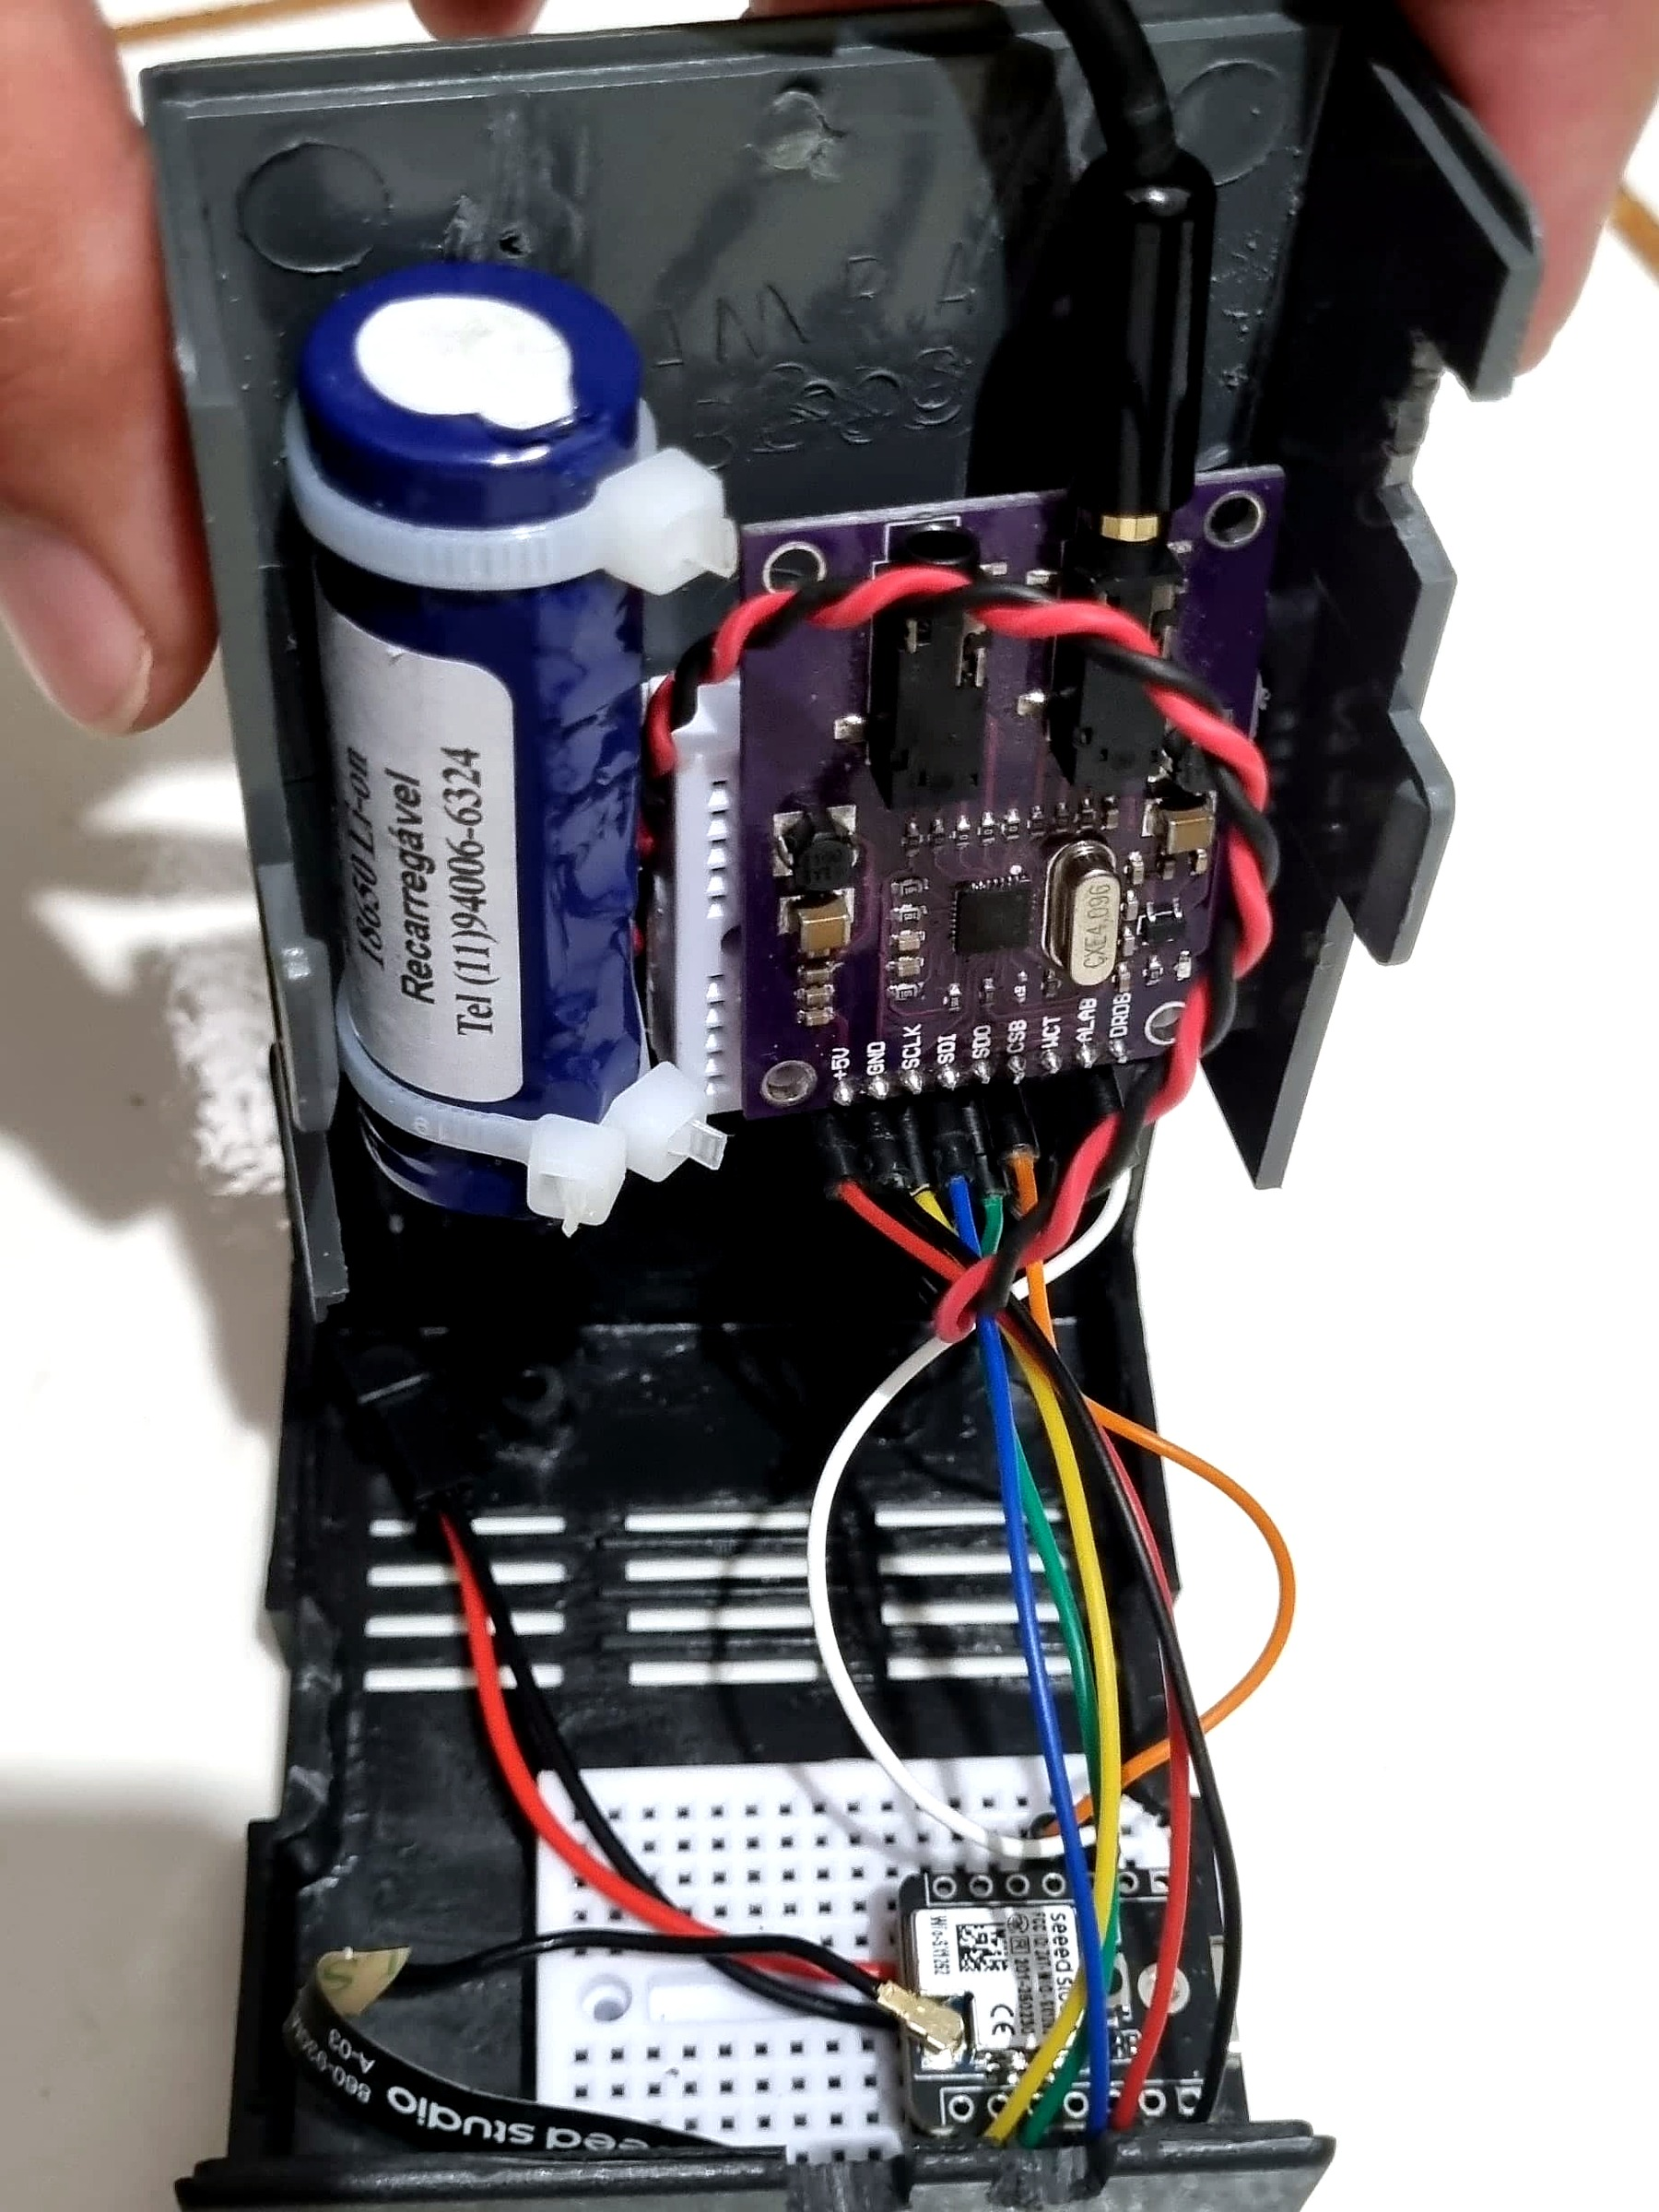
\includegraphics[width=0.30\linewidth]{assets/figura_03_prototipo_componentes_internos.jpg}}\hfill
\subfloat[Dispositivo montado e cabo de eletrodos]{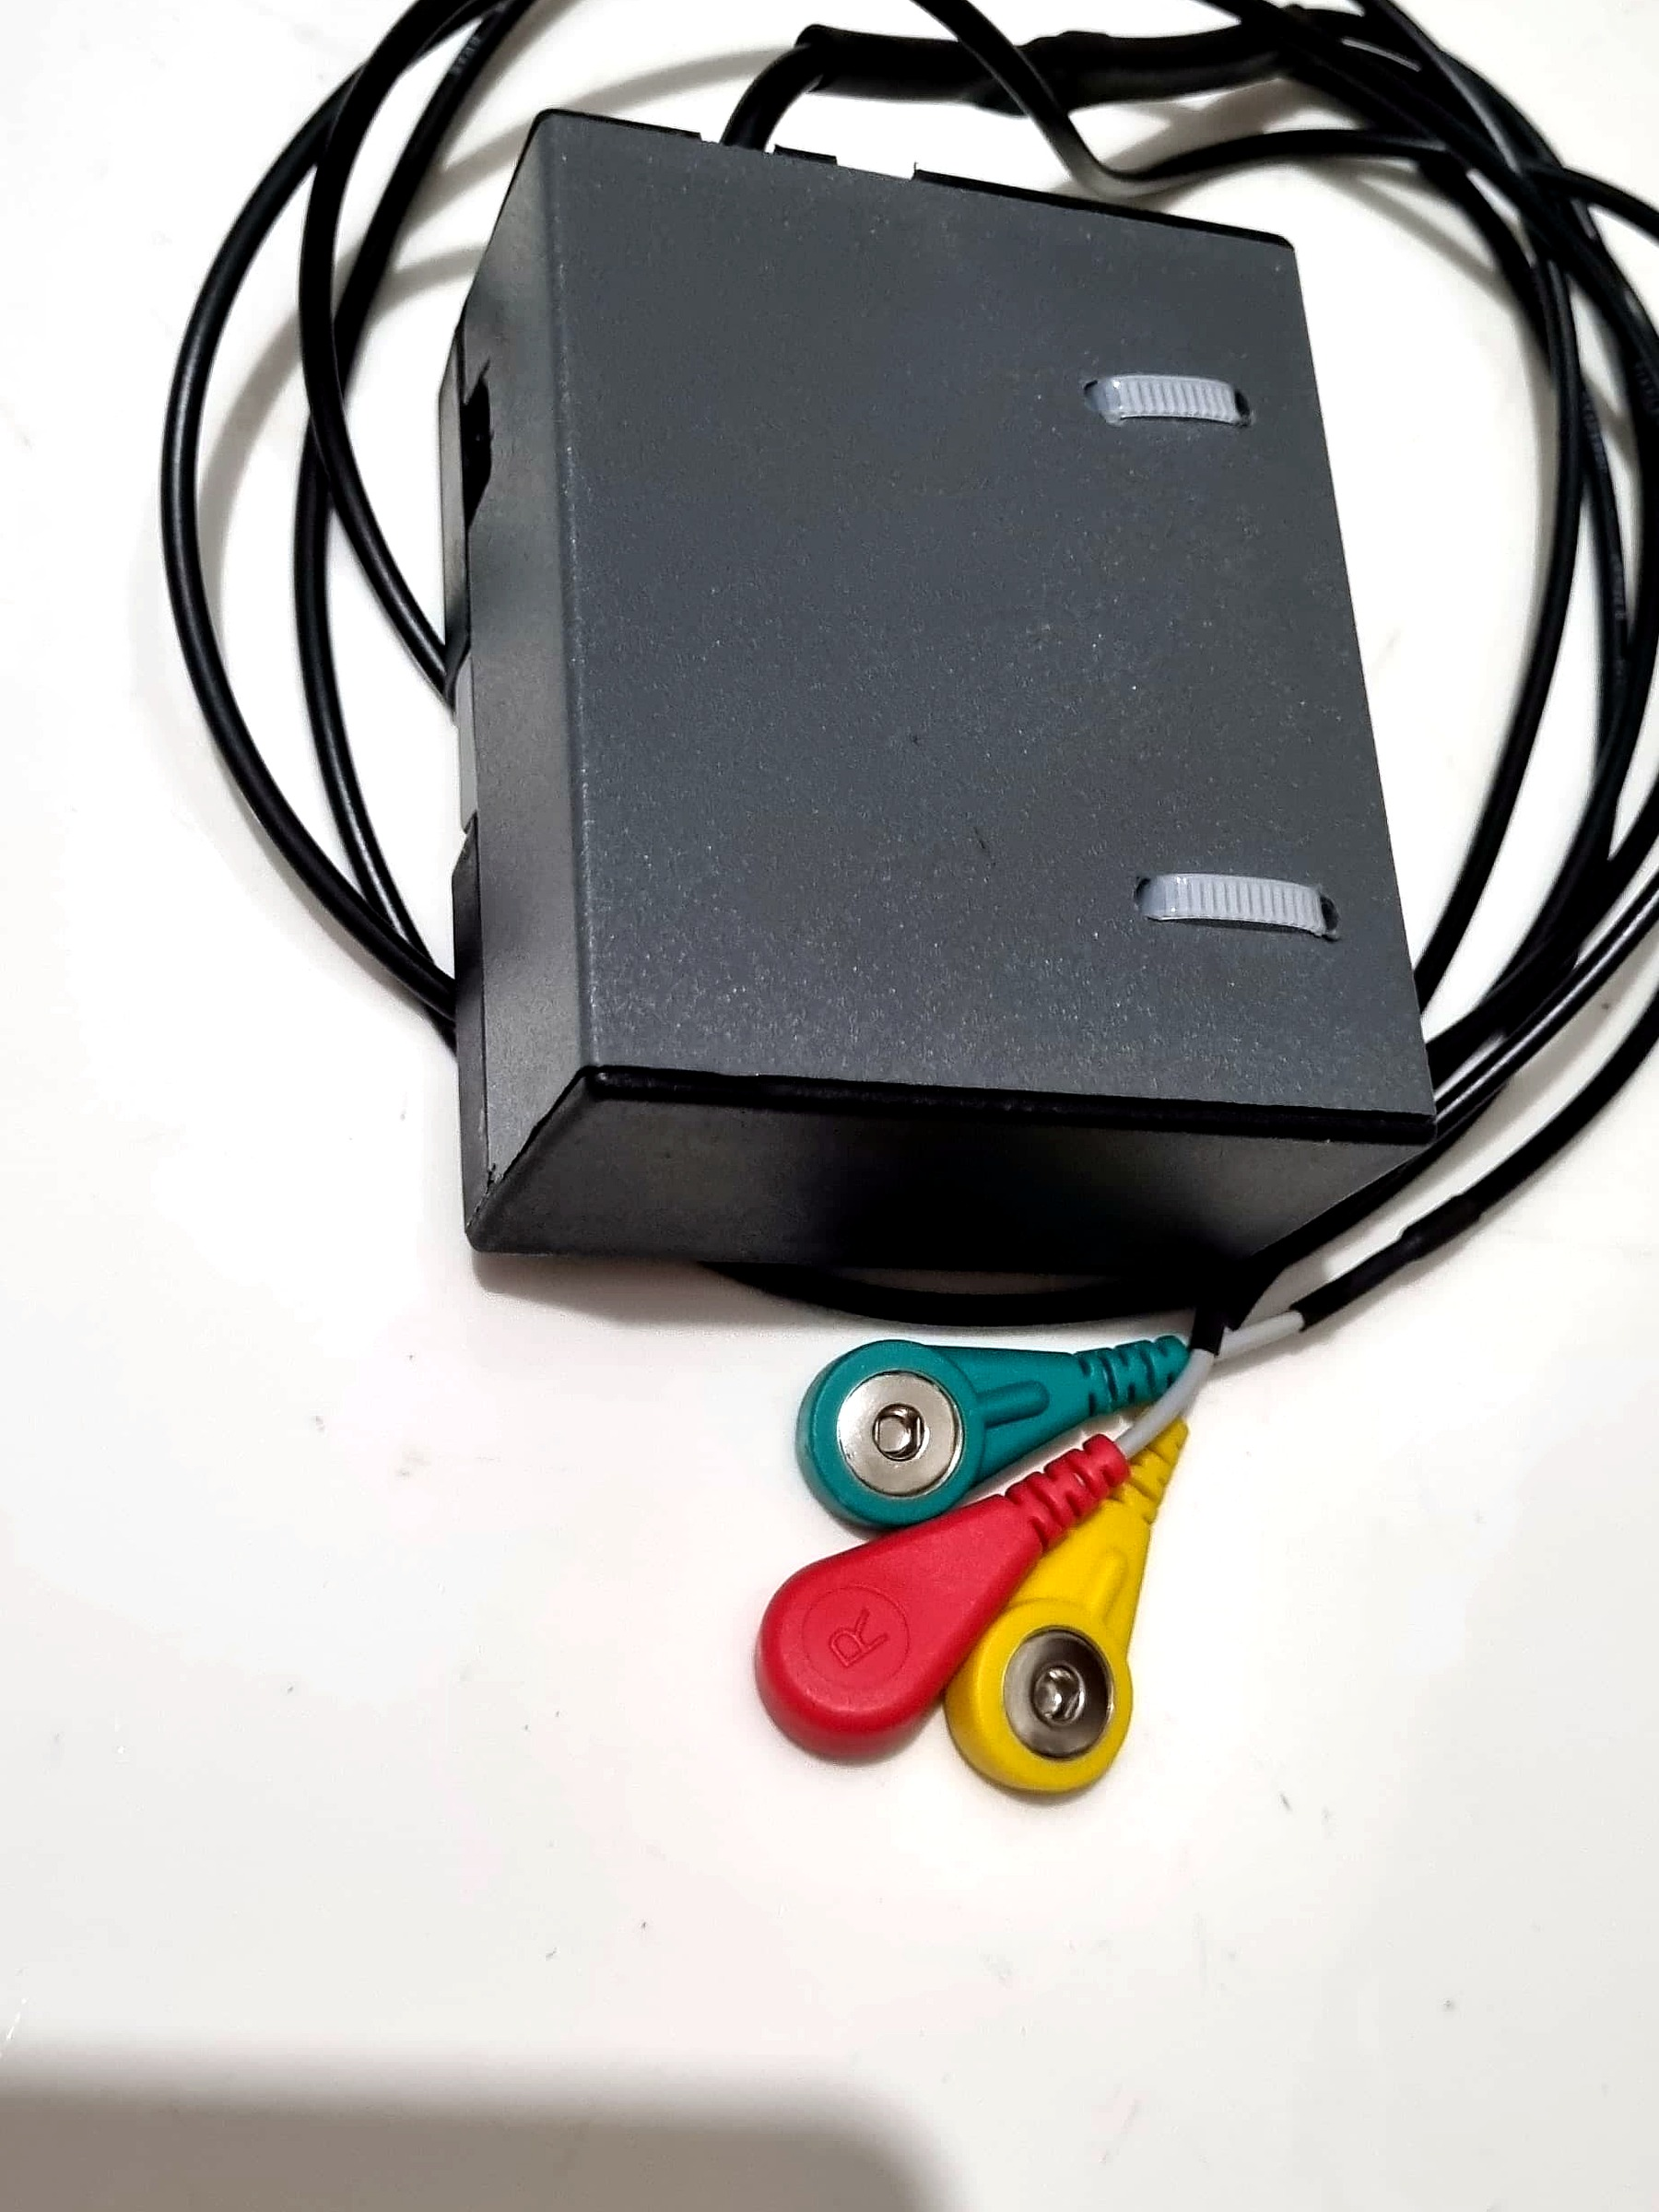
\includegraphics[width=0.30\linewidth]{assets/figura_01_prototipo_vista_superior_eletrodos.jpg}}\\[1ex]
\subfloat[Vista lateral: porta USB-C de recarga]{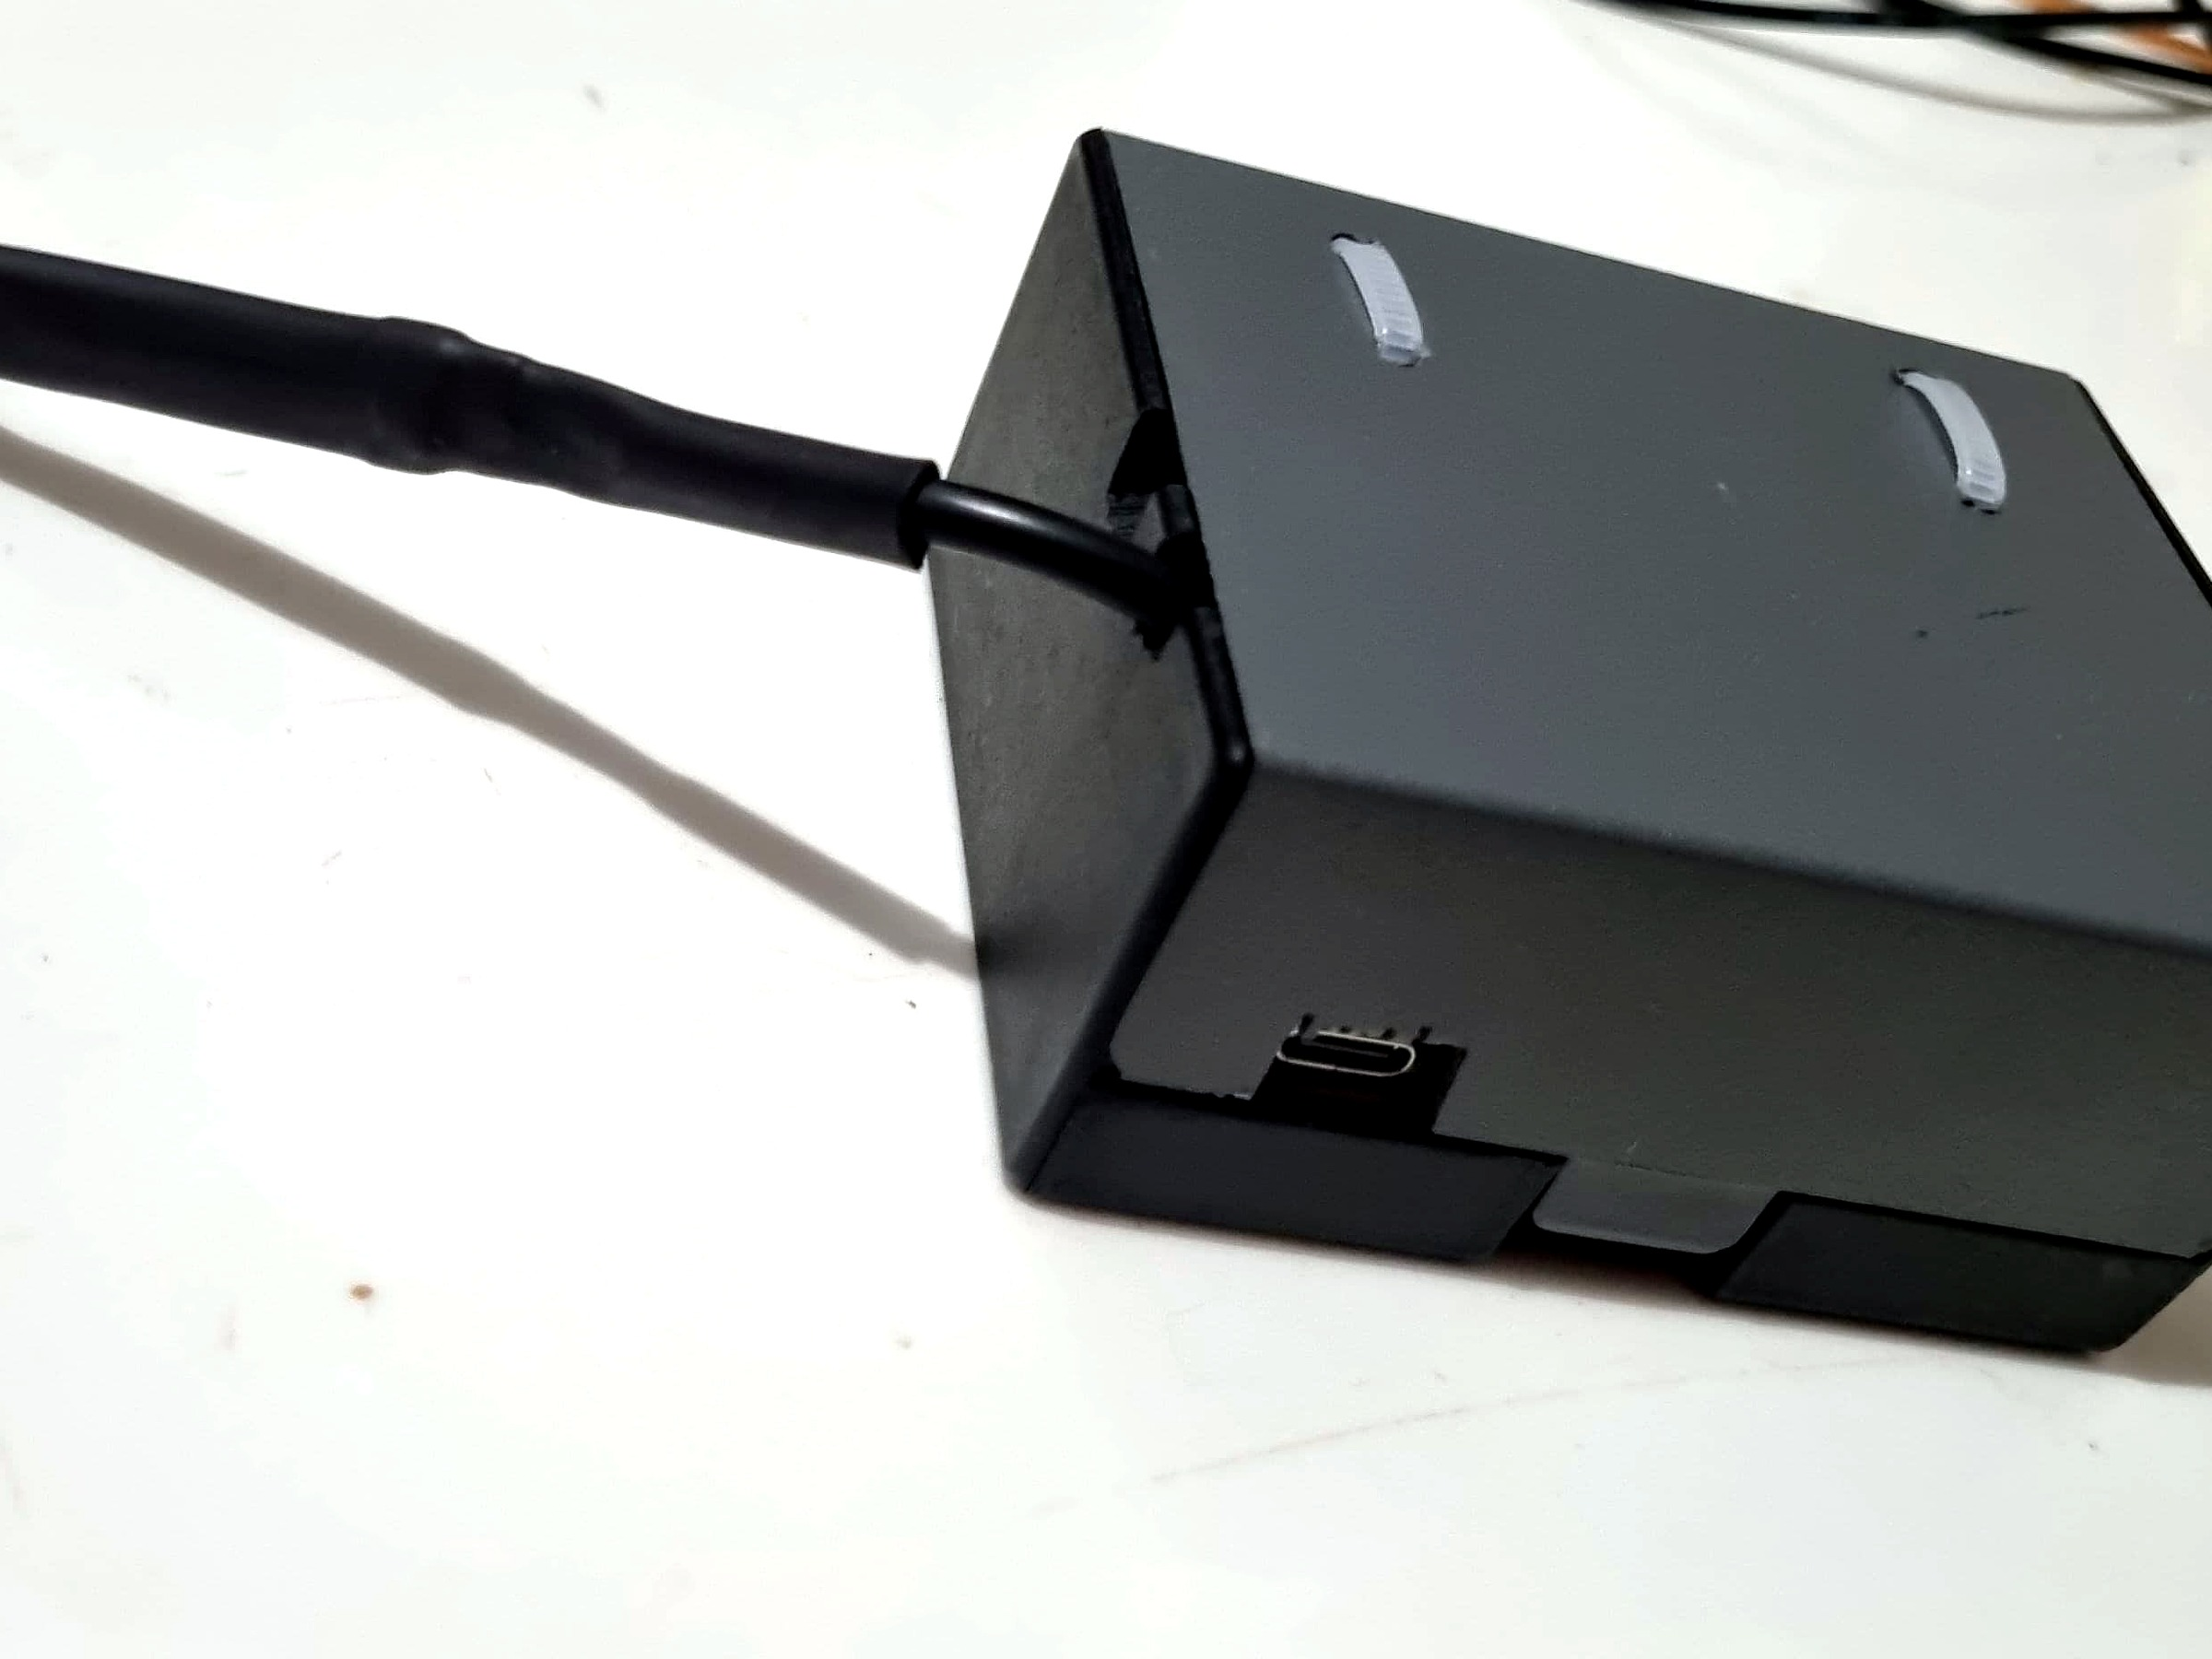
\includegraphics[width=0.55\linewidth]{assets/figura_02_prototipo_conector_usbc.jpg}}
\caption{Protótipo do dispositivo de aquisição de \acs{ECG}, encapsulado em caixa plástica comercial Patola\textsuperscript{\textregistered}, modelo PB-44: (a) vista interna, com a bateria de íons de lítio 18650 presa por abraçadeiras de náilon, a placa do \acs{AFE} CJMCU-1293 e, na base, o XIAO ESP32-S3 com o módulo Wio-SX1262 sobre matriz de contatos; (b) caixa fechada, com o cabo de três derivações e os eletrodos de pressão (\textit{snap}) nas cores do padrão IEC; (c) vista lateral, com o recorte da porta USB-C e a passagem do cabo de derivações.}
\label{fig:prototipo}
\end{figure}

\section{Desenvolvimento do Firmware Embarcado}
\label{sec:resFirmware}

O \textit{firmware} foi desenvolvido e encontra-se funcional em todas as suas etapas de processamento. A aquisição orientada a interrupção, disparada pelo sinal \acs{DRDY}, mostrou-se estável na taxa efetiva de 640 SPS (Seção~\ref{sec:resTaxa}), com leitura simultânea das três derivações pelo barramento \acs{SPI}. A cadeia de filtros digitais \acs{IIR} e o algoritmo de detecção de eventos foram implementados e executados sobre segmentos de 30~s armazenados na memória \textit{PSRAM} do microcontrolador, recurso que viabilizou o processamento de 19.200 amostras por segmento sem comprometer a memória interna.

O subsistema de armazenamento local em \textit{LittleFS} foi validado: para cada segmento processado, o resumo de 16 bytes foi gravado no \textit{log} binário, e a forma de onda dos segmentos sinalizados como anormais foi persistida integralmente, com as políticas de rotação operando conforme projetado. Os comandos de inspeção pela interface serial (despejo do \textit{log}, listagem e leitura dos arquivos de sinal bruto) permitiram auditar o conteúdo gravado e compará-lo com os dados recebidos na nuvem. O módulo de transmissão \textit{LoRaWAN}, baseado na biblioteca \textit{RadioLib}, realizou a montagem do \textit{payload} de 10 bytes e o envio na porta de aplicação 2, com a aquisição prosseguindo de forma independente do estado da conexão de rádio.

\section{Configuração da Rede LoRaWAN e Transmissão de Dados}
\label{sec:resTransmissao}

Inicialmente, realizou-se a configuração do \textit{gateway} da \textit{Radioenge} conectado ao \textit{Raspberry Pi 3} e a integração de um módulo Wio-SX1262 acoplado a um microcontrolador XIAO ESP32-S3. Essa integração facilitou os testes iniciais, permitindo direcionar os esforços para a comunicação com os servidores \textit{LoRaWAN}.

As primeiras tentativas de comunicação foram realizadas com a \acs{TTN}. Apesar de sua infraestrutura acessível e bem documentada, surgiram problemas recorrentes, como a exibição intermitente do dispositivo como \textit{offline}, mesmo com o envio de \textit{uplinks} válidos, além de latência variável na resposta dos pacotes e dependência integral de conectividade com a internet. A plataforma também impõe restrições à taxa de envio de mensagens (\textit{duty cycle}), dificultando aplicações que demandam transmissões frequentes.

Frente a essas dificuldades, a adoção de um servidor local com o \textit{ChirpStack} mostrou-se mais eficaz. A instalação local proporcionou maior controle sobre os componentes da rede, incluindo a visualização dos \textit{uplinks} em tempo real, a personalização dos parâmetros de recepção e a integração direta, via \acs{MQTT}, com a camada de aplicação. Embora tenha exigido uma curva de aprendizado mais acentuada, sobretudo na configuração dos perfis \acs{OTAA} e no roteamento interno dos dados, o servidor local demonstrou desempenho superior em termos de estabilidade e previsibilidade da comunicação.

Persistiram, contudo, desafios relacionados à natureza do protocolo \textit{LoRaWAN} em Classe~A, utilizado neste trabalho. Nesse modo, a abertura das janelas de recepção depende da transmissão anterior, o que limita substancialmente a taxa de envio. Em um dos experimentos, conduzido ainda sob a hipótese de transmitir a forma de onda, buscou-se enviar 15.000 amostras de \acs{ECG} comprimidas em blocos; embora a meta inicial fosse o envio de pacotes a cada 200 milissegundos, observou-se, na prática, intervalos entre 2 e 3 segundos por pacote, resultando em um tempo total de transmissão de aproximadamente 392,2 segundos — valor incompatível com aplicações em tempo quase real. Esse resultado, alinhado às restrições reportadas na literatura \citep{lorawanWaveform, 3-lead}, evidenciou a inviabilidade de transmitir a forma de onda completa e motivou a adoção da estratégia de detecção na borda, discutida na Seção~\ref{sec:resDeteccao}.

A banda AU915 (sub-banda 2) foi mantida ao longo de todos os testes, e o módulo Wio-SX1262 demonstrou compatibilidade e bom desempenho dentro das limitações do protocolo.

\section{Determinação da Taxa de Amostragem Efetiva}
\label{sec:resTaxa}

Durante a caracterização do ADS1293, constatou-se que a taxa de amostragem efetiva não correspondia ao valor anunciado pela biblioteca de controle. A configuração adotada é identificada na biblioteca como \texttt{SPS\_256} e ali documentada como 256 amostras por segundo\footnote{\textit{ProtoCentral ADS1293 ECG Library}, versão 1.3.0, de Protocentral Electronics, disponível em \url{https://github.com/Protocentral/protocentral-ads1293-arduino}. No arquivo \texttt{src/protocentral\_ads1293.h}, o comentário que acompanha a constante registra \texttt{SPS\_256, // R1=4, R2=5, R3=8 -> 102400/(4*5*8) = 256}: os fatores de decimação estão corretos, mas o quociente indicado não corresponde a eles.}. A contagem de amostras adquiridas no modo de diagnóstico do \textit{firmware}, contudo, indicou aproximadamente 1.920 amostras em 3~s, ou seja, cerca de 640 amostras por segundo --- duas vezes e meia o valor anunciado. A divergência importava porque os coeficientes dos filtros digitais e a conversão de amostras em tempo, da qual dependem os intervalos R-R, são calculados a partir dessa taxa.

Verificou-se, em seguida, qual das duas informações estava correta, recorrendo à cadeia de divisores do próprio conversor. Com a frequência de \textit{clock} interna $f_{CLK} = 409{,}6$~kHz, a frequência de modulação resulta em $f_{MOD} = f_{CLK}/4 = 102{,}4$~kHz, e a taxa de saída (\textit{Output Data Rate}) é dada pela Equação~\ref{eq:odr}:

\begin{equation}
    \text{ODR} = \frac{f_{MOD}}{R_1 \cdot R_2 \cdot R_3} = \frac{102{,}4 \times 10^3}{4 \cdot 5 \cdot 8} = 640 \text{ SPS}
    \label{eq:odr}
\end{equation}

\noindent em que $R_1$, $R_2$ e $R_3$ são os fatores de decimação configurados nos registradores do ADS1293. Os valores $R_1 = 4$, $R_2 = 5$ e $R_3 = 8$ são exatamente os que a biblioteca programa na configuração \texttt{SPS\_256}; aplicados à equação do manual do componente, resultam em 640~SPS, e não em 256. A divergência está, portanto, na nomenclatura e na documentação da biblioteca, e não entre teoria e medida: o valor calculado a partir dos registradores efetivamente programados coincide com o medido, e ambos estabelecem a taxa de amostragem efetiva do sistema em 640~SPS. Adotou-se esse valor em todo o processamento subsequente; mantida a taxa nominal de 256~SPS, as frequências de corte dos filtros e as estimativas de frequência cardíaca ficariam deslocadas pelo mesmo fator de 2,5.

\section{Aquisição do ECG Registrado no Próprio Autor}
\label{sec:resEcgProprio}

A primeira verificação da cadeia de aquisição foi feita sobre \acs{ECG} humano, registrado
no próprio autor. Ela não produz métrica de desempenho --- não há anotação de referência, e
o sujeito é um único indivíduo saudável ---, mas foi a etapa que revelou os dois defeitos
de aquisição corrigidos no trabalho e a limitação de especificidade do critério de arritmia
sinusal. Os traçados registrados não são reproduzidos neste texto: por se tratar de sinal
fisiológico humano, sua divulgação depende de apreciação por comitê de ética em pesquisa, à
qual o trabalho ainda não foi submetido. Relatam-se, portanto, apenas as grandezas
agregadas deles derivadas.

\subsection{Ausência de referência de modo comum e correção do acionamento de perna}
\label{sec:resSinal}

A aquisição do sinal foi avaliada por meio de uma ferramenta de visualização que recebe as três derivações pela interface serial do dispositivo. Nos ensaios preliminares, com o cabo de eletrodos posicionado segundo o triângulo de \textit{Einthoven}, o sinal capturado apresentou uma flutuação de baixa amplitude e frequência, sem as deflexões características do complexo QRS, da onda P e da onda T. Em consequência, o algoritmo de detecção não identificou picos R consistentes, sinalizando a maior parte dos segmentos como erro de processamento.

A investigação atribuiu o fenômeno à ausência de uma referência de modo comum efetiva: o amplificador de perna direita (\textit{Right-Leg Drive} -- RLD), necessário para estabilizar o potencial do corpo em relação ao circuito de entrada, não estava adequadamente conectado, deixando as entradas diferenciais sujeitas a interferência de modo comum. Como medida corretiva, adotou-se a configuração de \textit{driven-leg} de três eletrodos descrita na Seção~\ref{sec:cjmcu}, na qual a detecção de modo comum é realizada sobre os eletrodos RA e LL (\texttt{CMDET\_EN = 0x05}) e a contrarreação é reinjetada pelo eletrodo LA (\texttt{SELRLD = 010}).

A revalidação foi conduzida em um teste de bancada com o sistema conectado ao próprio autor. Registraram-se 30~s do sinal bruto de cada derivação, em modo de diagnóstico, sem filtragem. Nesse modo o \textit{firmware} imprime as três derivações a cada amostra, o que excede a capacidade do enlace serial (Seção~\ref{sec:resSerial}); por isso a ferramenta externa gravou 17.888 amostras no intervalo de 30~s --- cerca de 596 por segundo ---, e não as 19.200 que correspondem à taxa de conversão. A taxa do conversor é fixa em 640~SPS, imposta pelos divisores internos do ADS1293 (Seção~\ref{sec:resTaxa}); o que se reduz é o número de amostras que chegam ao computador, não a cadência com que o conversor as produz. Como a verificação se destinava à morfologia do traçado, e não à sua temporização, a perda não compromete a conclusão; a estimativa de frequência cardíaca dela derivada é, por essa razão, aproximada. Após a correção, a derivação II passou a exibir os complexos QRS de forma nítida e com a polaridade esperada, além das ondas P e T, permitindo a estimativa de uma frequência cardíaca em torno de 90~bpm.


Para quantificar o efeito do RLD sobre a interferência da rede elétrica, o teste foi repetido sob duas condições --- RLD ativo e RLD desconectado (\texttt{SELRLD = 000}) ---, mantendo-se inalterados os eletrodos, o seu posicionamento e o ambiente. Estimou-se, por análise espectral, a fração da energia total do sinal concentrada em torno de 60~Hz. Na derivação II, da qual o detector extrai os intervalos R-R, essa fração caiu de 0,081\,\% com o RLD desconectado para 0,019\,\% com o RLD ativo, redução de 4,3 vezes. Em valor absoluto, o valor eficaz da componente de 60~Hz passou de 0,0097 para 0,0053~mV, redução de 1,8 vezes --- a diferença entre as duas razões decorre de a energia total do sinal não ser idêntica nas duas aquisições. A Figura~\ref{fig:espectroRld} apresenta os dois espectros. Duas ressalvas delimitam o alcance da medida. Mesmo sem o RLD a energia de 60~Hz já era baixa, o que indica um ambiente eletromagneticamente favorável no ensaio; em instalações mais ruidosas espera-se benefício proporcionalmente maior do circuito. E trata-se de uma única aquisição de 30~s por condição, em um único ambiente: o valor quantifica o efeito observado nesta bancada, não uma figura de mérito do sistema.

\begin{figure}[htb]
\centering
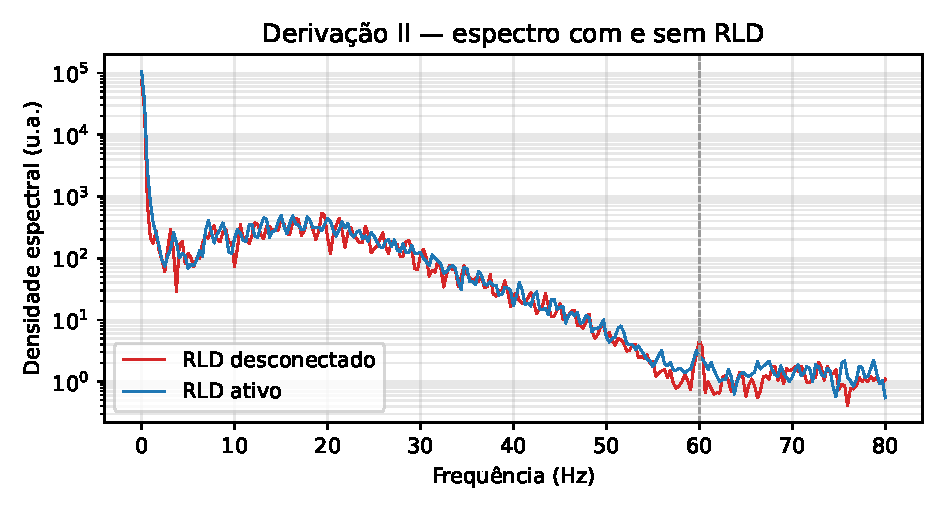
\includegraphics[width=0.9\textwidth]{assets/espectro_rld.pdf}
\caption{Espectro da derivação II no teste de bancada, com o RLD desconectado e ativo, estimado à taxa de amostragem do conversor (640~SPS). A linha tracejada indica a frequência da rede elétrica (60~Hz).}
\label{fig:espectroRld}
\end{figure}

Cabe destacar que a cadeia de condicionamento digital — composta pelos filtros passa-baixas (40~Hz) e passa-altas (0,5~Hz) descritos na Seção~\ref{sec:condicionamento} — foi assim avaliada sobre um sinal fisiológico real de boa qualidade, confirmando a remoção do desvio de linha de base e a preservação do complexo QRS de interesse.


\subsection{Especificidade do critério de arritmia sinusal em repouso}
\label{sec:resArritmia}

Além da validação da aquisição do sinal (Seção~\ref{sec:resSinal}), o algoritmo de detecção foi avaliado em um teste de bancada preliminar, com o sistema conectado ao próprio autor e a detecção ativa sobre segmentos de 30~s. Registraram-se sessões em duas posturas — em decúbito dorsal (repouso) e sentado. Os detectores de eventos clinicamente críticos — taquicardia, bradicardia, bloqueio e parada sinoatrial — não produziram falsos positivos em nenhuma das sessões. O detector de \textit{arritmia sinusal}, entretanto, sinalizou praticamente todos os segmentos.

A causa foi identificada no critério de decisão: o algoritmo marca o segmento como arritmia quando ocorre ao menos uma variação batimento-a-batimento do intervalo R-R superior a 120~ms. Em repouso, a arritmia sinusal respiratória — variação fisiológica e benigna do ritmo com a respiração, mediada pela modulação vagal do nó sinusal e acentuada pelo predomínio parassimpático nessa condição (\citeay{hrvTaskForce1996}; \citeay{guyton2021fisiologia}) — produziu, nas coletas desta bancada, cerca de 8 a 15 dessas variações por segmento de 30~s, de modo que o critério dispara em todos os segmentos. A rejeição dos batimentos eventualmente não detectados (intervalos R-R próximos ao dobro da mediana) removeu apenas uma fração das ocorrências, confirmando que a maior parte da variabilidade é de origem fisiológica.

A Tabela~\ref{tab:arritmiaPostura} resume a comparação entre as posturas. A frequência cardíaca elevou-se de cerca de 67~bpm, em repouso, para cerca de 92~bpm, na posição sentada, evidenciando que a aquisição acompanha corretamente a resposta autonômica; a taxa de segmentos sinalizados como arritmia, contudo, permaneceu elevada em ambas as condições, indicando que a manipulação postural não altera a especificidade do critério.

\begin{table}[htb]
\centering
\caption{Avaliação preliminar do detector de arritmia sinusal em duas posturas (teste de bancada, segmentos de 30~s).}
\label{tab:arritmiaPostura}
\begin{tabular}{l c c c}
\hline
\textbf{Condição} & \textbf{FC média} & \textbf{Variações R-R $>$120~ms} & \textbf{Segmentos} \\
                  & \textbf{(bpm)}    & \textbf{por segmento (média)}    & \textbf{sinalizados} \\
\hline
Decúbito (repouso) & $\approx$67 & $\approx$7,8 & 100\,\% \\
Sentado            & $\approx$92 & $\approx$8,6 & 100\,\% \\
\hline
\end{tabular}
\end{table}

Conclui-se que o critério de detecção de arritmia sinusal baseado na variabilidade do intervalo R-R apresenta especificidade intrinsecamente baixa para indivíduos saudáveis, uma vez que a arritmia sinusal respiratória constitui, ela própria, uma variação sinusal do ritmo. Trata-se de uma limitação conhecida da abordagem, e não de uma falha, portanto, a arritmia sinusal passou a ser tratada como informação de contexto, e não como alerta crítico, preservando-se como eventos críticos a taquicardia, a bradicardia e as pausas (bloqueio e parada sinoatrial), cuja detecção se mostrou específica. A caracterização quantitativa de sensibilidade e especificidade dessa e das demais classes, sobre sinais de classe conhecida, é apresentada nas Seções~\ref{sec:resEcgSintetico} e~\ref{sec:resEcgOrientadorFinal}, e sua generalização sobre a base anotada MIT-BIH, na Seção~\ref{sec:resMITBIH}.

Como medida de mitigação dessa limitação no nível da aplicação — sem alterar o critério de detecção na borda —, o aplicativo passou a exigir a confirmação por persistência antes de promover uma anomalia a alarme (Seção~\ref{sec:appFunc}). Os limiares padrão por classe constam da Tabela~\ref{tab:alarmePadrao}: a arritmia sinusal, por seu caráter fisiológico e recorrente, exige detecção em todos os dez últimos segmentos --- cerca de 5 minutos de persistência ---, ao passo que a parada sinoatrial alarma com uma única detecção. Dessa forma, reduz-se a taxa de alarmes falsos apresentada ao profissional, preservando-se integralmente o registro de todos os segmentos para análise posterior.

\section{Ensaios com ECG Sintetizado neste Trabalho}
\label{sec:resEcgSintetico}

Caracterizada a aquisição sobre \acs{ECG} humano, passou-se aos ensaios com \acs{ECG} de
classe conhecida, injetado na entrada do dispositivo pelo gerador de sinais descrito na
Seção~\ref{sec:validacaoGerador}. Os primeiros foram conduzidos sobre \acs{ECG} sintetizado
neste trabalho, escolha que tem uma razão de método: com o ritmo sob controle, qualquer
discrepância entre a classe esperada e a detectada só pode vir da cadeia de aquisição ou do
critério de decisão, e não do material de teste. Foi assim que se localizou o segundo
defeito de aquisição do trabalho.

\subsection{Saturação do enlace serial}
\label{sec:resSerial}

O primeiro dos dois defeitos foi identificado e corrigido durante estes ensaios com \acs{ECG} injetado de amplitude controlada. Constatou-se que a impressão contínua das três derivações pela interface serial, quando lida simultaneamente por uma ferramenta externa, exigia do enlace uma vazão superior à sua capacidade — cerca de 270~kbit/s contra os 230.400 bits por segundo configurados (Seção~\ref{sec:condicionamento}). Excedida a capacidade, a escrita bloqueava momentaneamente o laço de aquisição, reduzindo a taxa efetivamente registrada de 640 para cerca de 560 amostras por segundo. As amostras perdidas introduziam descontinuidades no \textit{buffer} que encurtavam artificialmente parte dos intervalos R-R e faziam o critério de variabilidade sinalizar arritmia de modo indevido, ainda que o sinal injetado fosse um ritmo regular. Ao desacoplar a saída de depuração da aquisição, por meio da decimação da impressão serial (Seção~\ref{sec:condicionamento}), o \textit{buffer} voltou a receber a totalidade das amostras: para um mesmo sinal normal injetado, os segmentos passaram a ser classificados corretamente como normais de forma consistente.

\subsection{Perda periódica de amostras na aquisição}
\label{sec:resPerdaAmostras}

Corrigida a saturação do enlace, restou um sintoma mais discreto: segmentos de ritmo normal continuavam a ser sinalizados como arritmia sinusal, de forma recorrente e sem que o \acs{ECG} injetado contivesse qualquer irregularidade. Duas hipóteses foram levantadas antes de se chegar à causa. A primeira atribuía o problema à frequência cardíaca do \acs{ECG} normal exatamente igual ao limiar: o traçado normal de 60~bpm possui R-R de exatamente 1000~ms, coincidente com o limiar de bradicardia, com margem nula; a adoção de um \acs{ECG} de 75~bpm (R-R de 800~ms, 200~ms de margem) eliminou as marcações indevidas de bradicardia, mas não as de arritmia. A segunda atribuía o problema à descontinuidade entre segmentos (Seção~\ref{sec:resProcedimento}), que a reprodução em laço introduz na junção entre o fim e o início do arquivo — como o arquivo tinha 30~s e o segmento de processamento também, ocorreria uma descontinuidade entre o final de um segmento gerado e o início do próximo; geraram-se então arquivos de 300~s, mas a hipótese foi refutada, pois 24 dos 30 segmentos continuaram a ser classificados erroneamente.

Esse resultado motivou o registro do sinal bruto adquirido. No traçado bruto (Figura~\ref{fig:perdaAmostras}), identificaram-se seis intervalos R-R anômalos, periódicos a cada aproximadamente 4,9~s, cada um com o intervalo de 800~ms reduzido para cerca de 710~ms. A causa foi localizada na aquisição, em um mecanismo distinto do da saturação serial (Seção~\ref{sec:resSerial}): agora com a saída de depuração já decimada, era a própria rotina de diagnóstico que consultava o espaço ocupado no sistema de arquivos local (\textit{LittleFS}) dentro do laço principal, a cada 5~s, bloqueando o processador por cerca de 105~ms; como a rotina de interrupção apenas sinaliza a disponibilidade de uma nova amostra, cerca de 66 amostras eram perdidas. O relatório de diagnóstico registrava 3.133 amostras válidas em vez das 3.200 esperadas — uma perda de 2,08\,\%, mais sutil que a da saturação serial (que reduzia a taxa a cerca de 560~SPS) e, por isso mesmo, mais difícil de identificar.

Ambos os problemas decorrem da mesma decisão de projeto: a rotina de interrupção associada ao sinal \acs{DRDY} apenas sinaliza a disponibilidade de uma nova amostra, e a leitura pelo barramento \acs{SPI} ocorre no laço principal. Nesse arranjo, a integridade da aquisição depende de o laço nunca bloquear por mais de um período de amostragem (1,56~ms a 640~SPS) --- condição silenciosamente violada pelas duas rotinas identificadas. O arranjo mais robusto é outro: executar a leitura do conversor dentro da própria rotina de interrupção, com prioridade máxima, gravando a amostra em memória antes de retornar; nesse caso, um bloqueio no laço atrasa o processamento, mas não descarta amostra alguma. Ele não foi adotado porque a leitura do \acs{AFE} é feita pela biblioteca de controle de terceiros empregada, cujas transações \acs{SPI} recorrem à interface padrão do \textit{framework} e não satisfazem os requisitos de execução em contexto de interrupção do ESP32, que exige que o código chamado resida na memória interna de instruções. Reescrever esse caminho implicaria substituir a biblioteca. Optou-se, em vez disso, por remover do laço as chamadas bloqueantes e por instrumentar a aquisição: o contador de interrupções \acs{DRDY} passou a ser comparado ao de leituras efetivadas, e a diferença entre ambos --- as amostras perdidas --- passou a constar do relatório de diagnóstico. Sob essa instrumentação, os ensaios subsequentes transcorreram sem perda registrada. A migração da leitura para a rotina de interrupção permanece como melhoria recomendada, por eliminar a falha por construção, e não por vigilância.

\begin{figure}[htbp]
\centering
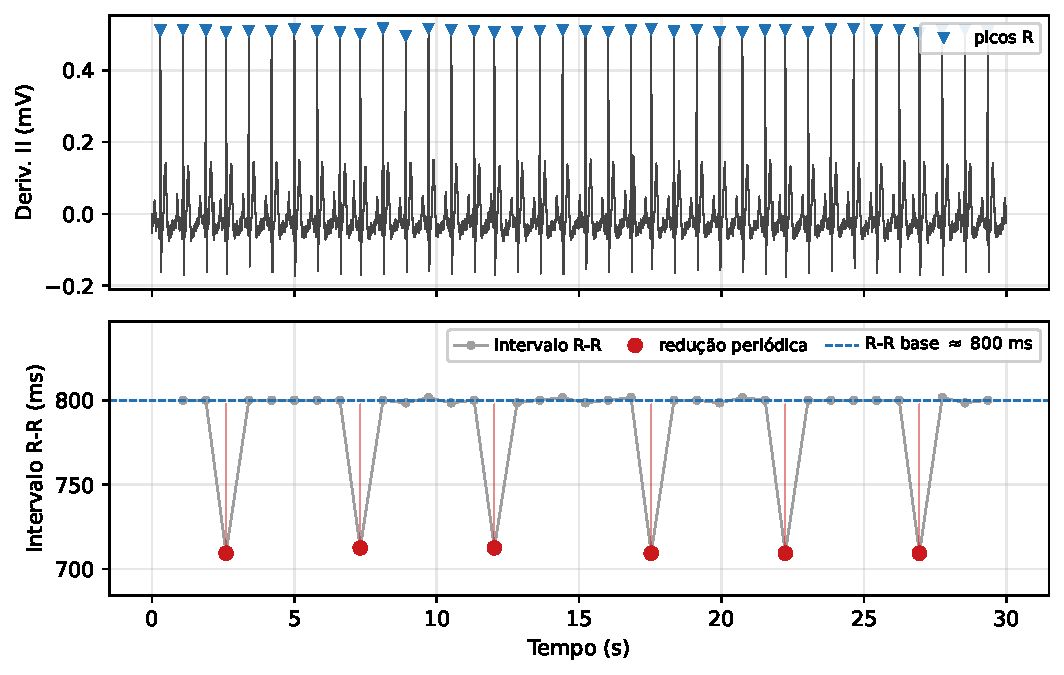
\includegraphics[width=0.95\linewidth]{assets/perda_amostras_rr.pdf}
\caption{Perda de amostras no sinal bruto de um segmento normal (75~bpm) indevidamente classificado como arritmia. Acima, a derivação II adquirida, com os picos R detectados; abaixo, a série de intervalos R-R, na qual se observam seis reduções periódicas — de $\approx$800 para $\approx$710~ms, a cada $\approx$4,9~s —, coincidentes com o bloqueio do laço de aquisição pela rotina de diagnóstico.}
\label{fig:perdaAmostras}
\end{figure}

Esse problema explicava todos os sintomas observados: a estimativa de frequência cardíaca cerca de 2\,\% maior; a aparente taxa de amostragem de 627~SPS, quando a taxa efetiva é de 640~SPS (Seção~\ref{sec:resTaxa}); e as marcações indevidas de arritmia, pois a diminuição periódica produzia variações R-R de 89 a 114~ms, muito próximas do limiar de 120~ms. A correção consistiu em remover do laço de aquisição a consulta ao sistema de arquivos.

\subsection{Desempenho sobre o ECG sintetizado e alcance do resultado}
\label{sec:resBateriaControlada}

Corrigida a aquisição, o ensaio foi repetido sobre um \acs{ECG} sintetizado de ritmo
estritamente controlado --- batimento obtido por soma de gaussianas, amplitude constante e
intervalos R-R distantes dos limiares de decisão ---, com 30 segmentos por classe e 180
ensaios no total. Os 180 segmentos foram classificados corretamente. O traçado normal, que
antes da correção era reconhecido em 20\,\% dos segmentos, passou a 100\,\%.

Esse resultado, entretanto, deve ser lido com três ressalvas, todas decorrentes do próprio
controle que o torna útil. O \acs{ECG} era sintético e de amplitude constante, e portanto
não exercitava o limiar global de amplitude do detector. Os intervalos R-R situavam-se
distantes dos limiares de decisão, o que dispensava a estimativa de qualquer precisão. E
cada intervalo R-R correspondia a um número inteiro de amostras --- 800~ms equivalem a
exatamente 512 amostras a 640~SPS ---, de modo que a quantização do instante do pico não
introduzia erro algum na estimativa da frequência cardíaca. Trata-se, portanto, do limite
superior do desempenho, obtido em condições deliberadamente favoráveis.

Para afastar as duas primeiras ressalvas sem perder o controle sobre o ritmo, sintetizou-se
um segundo conjunto, que adota como molde morfológico o batimento do \acs{ECG} cedido pelo
orientador e lhe impõe ritmo próprio: intervalo R-R de 800~ms (75~bpm) no traçado normal,
500~ms (120~bpm) na taquicardia e 1.200~ms (50~bpm) na bradicardia, com variabilidade
batimento a batimento de desvio-padrão de 15, 10 e 20~ms, respectivamente --- valores bem
abaixo do limiar de 120~ms do critério de arritmia sinusal, para não induzir classe falsa.
Sobre esse ritmo somaram-se imperfeições de amplitude, todas referidas à amplitude da onda
R: deriva senoidal de linha de base de 5\,\%, modulação respiratória de $\pm$8\,\% e ruído
branco de desvio-padrão de 2\,\%. Cabe registrar que apenas a \emph{morfologia} do batimento
provém do material externo; o ritmo e as pausas foram gerados aqui, de modo que as
limitações de ritmo do conjunto original, discutidas na Seção~\ref{sec:resModificacoes}, não
se transferem para este \acs{ECG}.

Sobre esse segundo conjunto, o sistema novamente classificou corretamente os 180 segmentos
(Tabela~\ref{tab:matrizFinal}), com as métricas por classe da
Tabela~\ref{tab:metricasClasse} e nenhum erro de processamento, o que indica integridade da
aquisição ao longo de todos os ensaios.

Cabe uma precisão sobre o alcance desse resultado, que diz respeito à regra de decisão
então vigente. Estes ensaios foram conduzidos sob o critério de pausa por duração absoluta,
e o \acs{ECG} de bloqueio foi construído para satisfazê-lo, com pausas na faixa de 4 a 6~s.
Sobre um ritmo de base de 800~ms, essas pausas equivalem a mais de cinco ciclos cardíacos,
de modo que a formulação relativa adotada depois (Seção~\ref{sec:resCriterioPausa}) as
classifica como \emph{parada sinusal}, e não como bloqueio. Reprocessado o mesmo arquivo
sob a regra final, as janelas de 30~s saem, de fato, como parada. A observação não aponta
defeito de detecção: ilustra que o material de teste acompanha a definição do critério, e
que a pausa de um bloqueio não se caracteriza por durar um certo número de segundos, mas
por fechar um número inteiro de ciclos do ritmo que a precede. É o mesmo fenômeno que, em
sentido inverso, impedia o reconhecimento das pausas do \acs{ECG} cedido pelo orientador
(Seção~\ref{sec:resOrigLimpo}).

\begin{table}[htb]
\centering
\caption{Matriz de confusão dos ensaios sobre o \acs{ECG} sintetizado neste trabalho (30 segmentos por classe; linha = classe esperada, coluna = classe detectada).}
\label{tab:matrizFinal}
\begin{tabular}{l c c c c c c}
\hline
\textbf{Esperada / Detectada} & \textbf{Normal} & \textbf{Taqui.} & \textbf{Bradi.} & \textbf{Arrit.} & \textbf{Bloq.} & \textbf{Parada} \\
\hline
Normal            & 30 & 0  & 0  & 0  & 0  & 0  \\
Taquicardia       & 0  & 30 & 0  & 0  & 0  & 0  \\
Bradicardia       & 0  & 0  & 30 & 0  & 0  & 0  \\
Arritmia sinusal  & 0  & 0  & 0  & 30 & 0  & 0  \\
Bloqueio sinoatr. & 0  & 0  & 0  & 0  & 30 & 0  \\
Parada sinoatr.   & 0  & 0  & 0  & 0  & 0  & 30 \\
\hline
\end{tabular}
\end{table}

\begin{table}[htb]
\centering
\caption{Desempenho de detecção por classe sobre o \acs{ECG} sintetizado neste trabalho (valores em \%).}
\label{tab:metricasClasse}
\begin{tabular}{l c c c c c c}
\hline
\textbf{Classe} & \textbf{N} & \textbf{Sens.} & \textbf{Espec.} & \textbf{\acs{VPP}} & \textbf{\acs{VPN}} & \textbf{Taxa de acerto} \\
\hline
Normal            & 30 & 100,0 & 100,0 & 100,0 & 100,0 & 100,0 \\
Taquicardia       & 30 & 100,0 & 100,0 & 100,0 & 100,0 & 100,0 \\
Bradicardia       & 30 & 100,0 & 100,0 & 100,0 & 100,0 & 100,0 \\
Arritmia sinusal  & 30 & 100,0 & 100,0 & 100,0 & 100,0 & 100,0 \\
Bloqueio sinoatr. & 30 & 100,0 & 100,0 & 100,0 & 100,0 & 100,0 \\
Parada sinoatr.   & 30 & 100,0 & 100,0 & 100,0 & 100,0 & 100,0 \\
\hline
\end{tabular}
\end{table}

Diferentemente do ensaio anterior, o erro de estimativa da frequência cardíaca não foi nulo
(Tabela~\ref{tab:erroFC}), o que era esperado diante da variabilidade imposta aos intervalos
R-R. O erro absoluto médio permaneceu, ainda assim, abaixo de 0,5~bpm nas três classes de
ritmo regular, com erro máximo de 1~bpm --- margem confortável frente ao limite admitido
para medidores de frequência cardíaca, de $\pm$10\,\% da frequência de entrada ou
$\pm$5~bpm, prevalecendo o maior (AAMI, \citeyear{aamiEC13}); a exatidão do medidor de
frequência cardíaca é também objeto da norma particular dos equipamentos de monitorização
de \acs{ECG} (IEC, \citeyear{iec6060127}). As classes de arritmia e de pausa foram omitidas
desta análise por não possuírem frequência cardíaca regular ao longo de todo o segmento.

\begin{table}[htb]
\centering
\caption{Erro de estimativa da frequência cardíaca nas classes de ritmo regular, sobre o \acs{ECG} sintetizado neste trabalho (em bpm).}
\label{tab:erroFC}
\begin{tabular}{l c c c c}
\hline
\textbf{Classe} & \textbf{N} & \textbf{Erro médio abs.} & \textbf{Erro máx.} & \textbf{Desvio-padrão} \\
\hline
Normal      & 30 & 0,4 & 1,0 & 0,5 \\
Taquicardia & 30 & 0,2 & 1,0 & 0,4 \\
Bradicardia & 30 & 0,5 & 1,0 & 0,5 \\
\hline
\end{tabular}
\end{table}

Cabe uma ressalva final. O reconhecimento integral do \acs{ECG} normal nestes ensaios não
contradiz a baixa especificidade do critério de arritmia sinusal caracterizada na
Seção~\ref{sec:resArritmia}. O \acs{ECG} normal sintetizado possui variabilidade R-R
limitada --- variação inferior ao limiar de 120~ms ---, ao passo que o \acs{ECG} de um
indivíduo real em repouso exibe arritmia sinusal respiratória de amplitude suficiente para
satisfazer o critério. A limitação manifesta-se sobre sinal fisiológico humano, não sobre
\acs{ECG} controlado.

\section{Ensaios com o ECG Cedido pelo Orientador: Versão Original do Algoritmo}
\label{sec:resEcgOrientadorOriginal}

As duas etapas anteriores empregaram \acs{ECG} de origem própria --- registrado no autor ou
sintetizado aqui. Esta emprega material independente: seis arquivos de \acs{ECG} sintético,
um por classe, cedidos pelo orientador, com complexo P-QRS-T invariante ao longo do registro
e ritmo especificado por ele. A independência importa porque remove do autor a escolha do
material com que o seu próprio sistema é avaliado. Os ensaios desta seção foram conduzidos
sobre a \emph{versão original} do algoritmo de detecção, tal como cedido por seus autores,
e é por isso que eles expõem as limitações que a Seção~\ref{sec:resModificacoes} consolida.

\subsection{Desempenho sobre ECG sem ruído}
\label{sec:resOrigLimpo}

As quatro classes definidas pelo ritmo --- normal a 63~bpm, taquicardia a 105~bpm,
bradicardia a 57~bpm e arritmia sinusal com variação R-R de 130~ms --- foram reproduzidas
pelo gerador e processadas em 30 segmentos cada, totalizando 120 ensaios. Todos os 120 foram
classificados corretamente, sem erro de processamento, e o erro absoluto médio de estimativa
da frequência cardíaca foi nulo nas quatro classes. Esse erro nulo não é mérito do
estimador, e convém dizê-lo: o \acs{ECG} cedido é exatamente periódico, de modo que a
frequência de referência é um valor único e a estimativa o reproduz sem resíduo. A medida
representativa do erro sob ritmo variável é a da Seção~\ref{sec:resBateriaControlada}, entre
0,2 e 0,5~bpm.

As duas classes de pausa não puderam ser ensaiadas com os arquivos originais, e a razão é o
próprio critério então vigente. O algoritmo definia bloqueio e parada por \emph{duração
absoluta} da pausa: exigia ao menos duas pausas entre 4 e 6~s para o bloqueio sinoatrial, e
uma pausa acima de 6~s para a parada sinusal. As pausas dos arquivos cedidos foram
construídas, corretamente, como múltiplos do intervalo R-R de base --- 1.904~ms
($2\times$952) e 2.856~ms ($3\times$952) no bloqueio, 3.332~ms ($3{,}5\times$952) na parada
---, que é a representação fisiológica do quadro: no bloqueio sinoatrial de segundo grau o
impulso é barrado e a pausa fecha em número inteiro de ciclos. Nenhuma delas alcança o piso
de 4~s. Em ensaio prévio de duas repetições por classe, os segmentos saíram com máscara
\texttt{0x06} --- bradicardia acompanhada de arritmia --- e foram rotulados como
bradicardia, sem qualquer detecção de pausa. O resultado é determinístico, e não amostral:
decorre da comparação entre a duração das pausas do arquivo e o piso do critério, de modo
que repetir o ensaio 30 vezes produziria trinta vezes o mesmo desfecho. Optou-se por não
comprometer as horas de bancada para reproduzi-lo.

Para fechar as seis classes sob o critério absoluto, os dois \acs{ECG} de pausa foram
remontados com material do próprio arquivo cedido: como o \acs{ECG} dele é exatamente
periódico e tem linha de base nula, cada segmento foi montado como uma sequência de
posições de um ciclo, em que cada posição recebe ou um batimento recortado do seu arquivo
normal, ou um ciclo de silêncio. Nada foi sintetizado; alterou-se apenas quantos ciclos de
silêncio separam dois batimentos, de modo a produzir pausas de $5\times$R-R (4.760~ms) e de
$7\times$R-R (6.664~ms), que recaem dentro da faixa absoluta exigida. Sobre esses dois
\acs{ECG}, as duas classes de pausa foram reconhecidas nos 30 segmentos cada, com 60 ensaios
sem erro de processamento.

Cabe registrar a fragilidade dessa evidência, e ela é de princípio: um \acs{ECG} construído
por quem também escolhe o critério demonstra que a cadeia reproduz e classifica a pausa, não
que o detector reconheça pausas arbitrárias. O desfecho relevante desta etapa não é,
portanto, a taxa de acerto, mas a constatação que a precedeu --- o critério por duração
absoluta obrigava a distorcer o material de teste para que ele caiba na regra, em vez de
reconhecer o quadro clínico tal como ele se apresenta. Foi essa constatação que motivou a
revisão descrita na Seção~\ref{sec:resCriterioPausa}.

\subsection{Desempenho sob ruído somado}
\label{sec:resRuido}

Os ensaios anteriores empregaram \acs{ECG} livre de ruído, adequado para isolar o comportamento do detector frente ao ritmo, mas distante das condições de aquisição em campo. Para caracterizar a robustez do sistema a interferências, somou-se ruído sintético ao \acs{ECG} das seis classes, reproduzindo o ensaio conduzido por \citeay{moraesFirmwareECG}. Foram consideradas três perturbações --- uma senoide de 0,33~Hz, que simula a deriva da linha de base pela respiração; uma senoide de 60~Hz, que simula a interferência da rede elétrica; e um ruído aleatório de banda larga, que simula os artefatos de movimento e de atividade muscular ---, cada uma somada em três amplitudes, correspondentes a 10, 20 e 30\,\% da excursão pico-a-vale do sinal sem ruído. A combinação das seis classes com os três tipos de perturbação e as três amplitudes resultou em 54 condições distintas que, a 30 repetições cada, totalizaram 1.620 ensaios. Nenhum ensaio retornou erro de processamento.

A Figura~\ref{fig:ruidoTipos} ilustra os três tipos de perturbação, na maior amplitude, somados ao \acs{ECG} normal. A Tabela~\ref{tab:ruidoAcuracia} resume a taxa de acerto por condição. A taxa de acerto total foi de 93,5\,\% (1.515 dos 1.620 ensaios).

\begin{figure}[htbp]
\centering
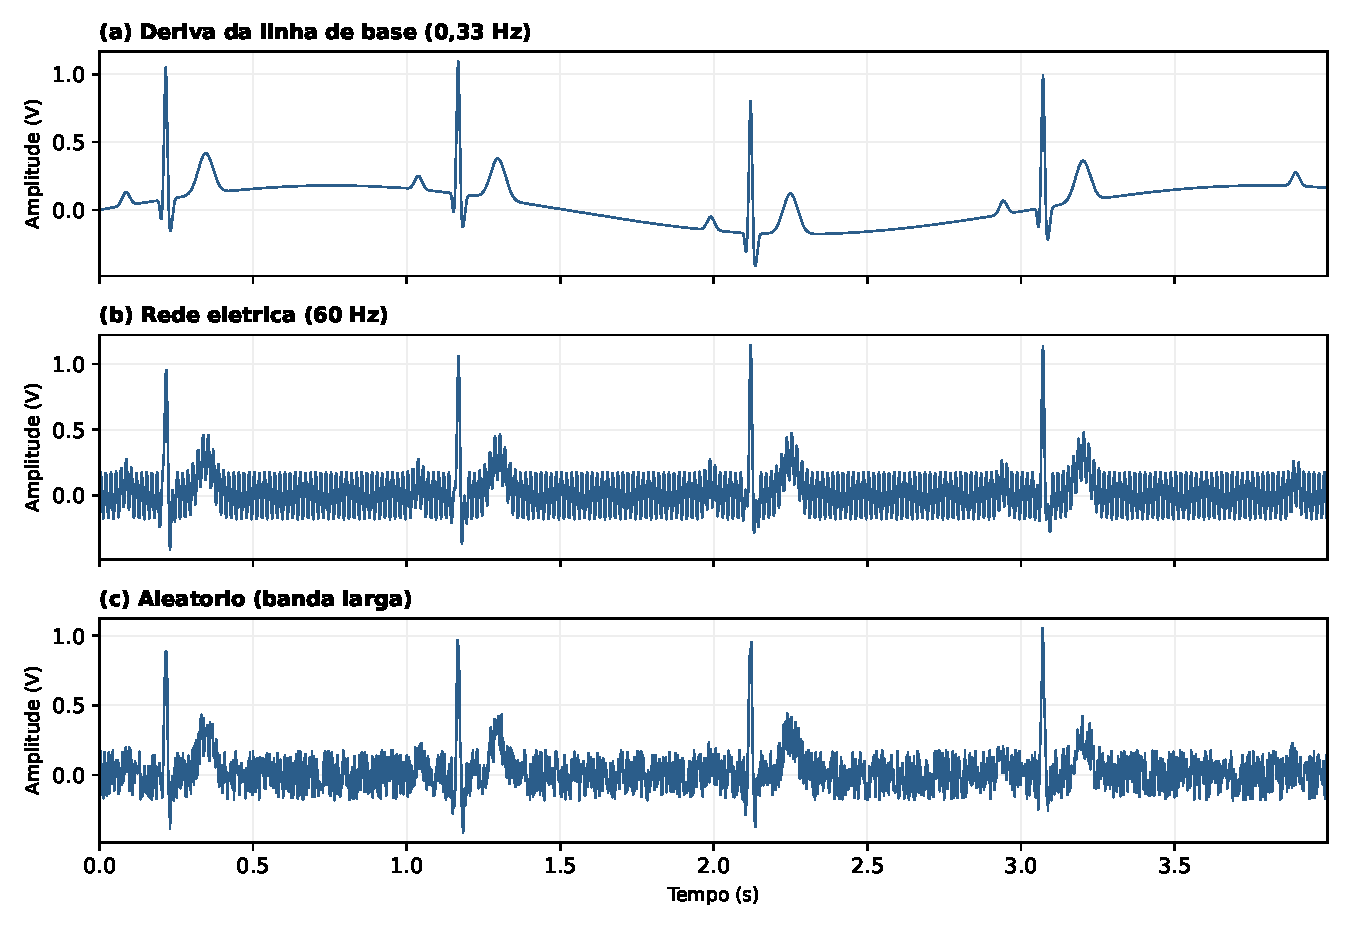
\includegraphics[width=\linewidth]{assets/figura_ruido_tipos.pdf}
\caption{\acs{ECG} normal com cada um dos três tipos de ruído somado a 30\,\% da excursão do sinal: (a) deriva da linha de base a 0,33~Hz; (b) interferência de rede a 60~Hz; (c) ruído aleatório de banda larga. Trecho de 4~s.}
\label{fig:ruidoTipos}
\end{figure}

A deriva de 0,33~Hz não produziu erro algum em nenhuma amplitude, resultado esperado, uma vez que sua frequência situa-se abaixo do corte do filtro passa-alta de 0,5~Hz do \textit{firmware} e é, portanto, atenuada antes da detecção. O ruído aleatório degradou o desempenho apenas na maior amplitude, e ainda assim de forma parcial (92,2\,\% a 30\,\%): a única classe afetada foi a normal, na qual a perturbação de banda larga ocasionalmente introduz um pico indesejado que eleva a variabilidade R-R acima do limiar de arritmia. Trata-se da mesma condição em que \citeay{moraesFirmwareECG} registraram o único resultado inconsistente do algoritmo original --- ruído aleatório na amplitude de 30\,\% ---, ainda que a manifestação difira: ali a taxa de acerto caiu a 98,33\,\% na detecção de bloqueio sinoatrial, com sensibilidade de 90\,\%, por \emph{perda} de picos R; aqui, a falha decorre da introdução de um pico \emph{indesejado} sobre o traçado normal. O que se repete, portanto, não é o desfecho, mas a natureza da limitação e o patamar em que ela se manifesta: a localização dos complexos pelo método da operação de diferenças degrada-se sob ruído de banda larga a partir de 30\,\% da excursão, amplitude que os próprios autores identificam como aquela em que o algoritmo "apresentou certa dificuldade na detecção dos picos R".

A divergência quanto à classe afetada encontra explicação no escopo distinto dos dois experimentos. Os ensaios de \citeay{moraesFirmwareECG} alimentaram o algoritmo diretamente com vetores de amostras produzidos por programa, aos quais o ruído fora somado --- de modo que a perturbação vista pelo detector é exatamente a especificada. Nos ensaios aqui relatados, o \acs{ECG} perturbado é reproduzido fisicamente e percorre o divisor resistivo, o \acs{AFE}, a quantização a 640~SPS e a cascata de filtros antes de alcançar o detector; o passa-baixas de 40~Hz remove parte da banda larga, ao passo que a cadeia analógica acrescenta seu próprio resíduo. O ruído que chega ao algoritmo não é, portanto, o mesmo, ainda que a especificação de amplitude o seja. As duas medidas não se contradizem: uma caracteriza o \emph{algoritmo} isoladamente, a outra o \emph{sistema} que o incorpora, e é a segunda que interessa ao propósito desta dissertação.

\begin{table}[htb]
\centering
\caption{Taxa de acerto por condição de ruído (seis classes, 30 repetições cada; 180 ensaios por célula).}
\label{tab:ruidoAcuracia}
\begin{tabular}{l c c c}
\hline
\textbf{Perturbação} & \textbf{10\,\%} & \textbf{20\,\%} & \textbf{30\,\%} \\
\hline
Deriva (0,33~Hz)  & 100,0\,\% & 100,0\,\% & 100,0\,\% \\
Rede (60~Hz)      & 100,0\,\% & 100,0\,\% & 50,0\,\%  \\
Aleatório         & 99,4\,\%  & 100,0\,\% & 92,2\,\%  \\
\hline
\end{tabular}
\end{table}

O único ponto de falha expressivo ocorreu sob a interferência de rede de 60~Hz na amplitude de 30\,\%, em que a taxa de acerto caiu a 50\,\%. A Tabela~\ref{tab:rede30Classe} discrimina esse caso por classe: as classes normal, taquicardia e arritmia sinusal deixaram de ser reconhecidas por completo, ao passo que a bradicardia, o bloqueio e a parada sinoatrial permaneceram em 100\,\%. A falha decorre da perda de picos R: sob a interferência, o detector deixa de registrar parte dos complexos, o que eleva o intervalo R-R médio — o erro absoluto médio de estimativa do intervalo, inferior a 1\,\% em todas as demais condições, atinge 22\,\% nesta — e desloca a classificação para bradicardia ou arritmia. As classes preservadas são justamente aquelas cujo diagnóstico não depende da contagem exata de picos, mas da presença de pausas longas (bloqueio e parada) ou de um ritmo lento já distante dos demais limiares (bradicardia).

\begin{table}[htb]
\centering
\caption{Classificação por classe sob interferência de rede de 60~Hz a 30\,\% de amplitude (30 repetições por classe).}
\label{tab:rede30Classe}
\begin{tabular}{l c c}
\hline
\textbf{Classe} & \textbf{Acertos} & \textbf{Resultado} \\
\hline
Normal            & 0/30  & classificada como bradicardia/arritmia \\
Taquicardia       & 0/30  & classificada como arritmia \\
Bradicardia       & 30/30 & correta \\
Arritmia sinusal  & 0/30  & classificada como bradicardia \\
Bloqueio sinoatr. & 30/30 & correta \\
Parada sinoatr.   & 30/30 & correta \\
\hline
\end{tabular}
\end{table}

\section{Limitações Identificadas e Modificações Implementadas}
\label{sec:resModificacoes}

Os ensaios relatados até aqui expuseram limitações de três naturezas distintas, e convém
separá-las antes de tratar das correções. Algumas pertencem à \emph{cadeia de aquisição}
desenvolvida nesta dissertação, como a perda periódica de amostras
(Seção~\ref{sec:resPerdaAmostras}); foram corrigidas no \textit{firmware} e já se relatou
como. Outras pertencem ao \emph{procedimento de ensaio}, como a descontinuidade introduzida
pela reprodução em laço, e dizem respeito à validade da medida, não ao sistema medido. As
demais pertencem à \emph{regra de decisão} do algoritmo reaproveitado, e a sua correção
exigiu alterar código de terceiros --- o que foi feito sob orientação dos autores, com o
cuidado de preservar a comparabilidade com a versão original.

Esta seção reúne as do segundo e do terceiro grupos. A regra de decisão foi revista em
quatro etapas, cada uma decorrente de um defeito identificado na anterior: o critério de
pausa passou a ser expresso como proporção do ritmo de base, o critério de arritmia sinusal
ganhou um limite superior, uma varredura sistemática revelou faixas de intervalo longo não
cobertas por critério algum e, para elas, acrescentou-se uma sexta categoria de
anormalidade. Avaliou-se ainda um filtro rejeita-faixa para a interferência de rede, que não
foi adotado. As subseções seguintes tratam de cada uma, e a
Seção~\ref{sec:resEcgOrientadorFinal} mede o resultado do conjunto sobre o mesmo \acs{ECG}
da Seção~\ref{sec:resEcgOrientadorOriginal}.

\subsection{Critério de pausa: da duração absoluta à razão com o ritmo de base}
\label{sec:resCriterioPausa}

A versão original definia o bloqueio sinoatrial por uma faixa absoluta de duração --- ao
menos duas pausas entre 4 e 6~s no mesmo segmento --- e a parada sinusal por uma pausa acima
de 6~s. O problema dessa formulação apareceu na Seção~\ref{sec:resOrigLimpo} e é de
princípio, não de calibração: a pausa que caracteriza essas condições não tem duração
própria, e sim proporção com o ritmo que a precede. Uma pausa de 2~s é um batimento
suprimido em quem está a 60~bpm e dois batimentos suprimidos em quem está a 120~bpm; é
bloqueio no primeiro caso e nada no segundo. Um piso fixo de 4~s, por sua vez, só reconhece
pausas que, em ritmo normal, equivalem a quatro ciclos ou mais --- muito além do que a
definição clínica exige.

O critério foi então reformulado, por determinação do orientador, em termos relativos ao
intervalo R-R de base do segmento, tomado como a \emph{mediana} dos intervalos --- estatística
robusta às próprias pausas, que na média puxariam a referência para cima e encolheriam a
razão. O bloqueio sinoatrial de segundo grau passou a ser reconhecido quando um intervalo
equivale a dois ou três ciclos do ritmo de base, com tolerância de 5\,\% em torno do
múltiplo, o que corresponde à supressão de um ou de dois complexos, com retomada do ritmo; a
parada sinusal, quando o intervalo excede três ciclos. Não há mais piso absoluto de duração.

A evidência do efeito dessa revisão é direta, e vem de uma comparação em que apenas a regra
mudou. Os arquivos de bloqueio e de parada cedidos pelo orientador, cujas pausas de 1,9 a
3,3~s não alcançavam o piso de 4~s e que por isso não eram reconhecidos
(Seção~\ref{sec:resOrigLimpo}), foram reproduzidos sem qualquer alteração sob o critério
revisto: as duas classes passaram a ser reconhecidas em todos os 30 segmentos cada. Nenhuma
característica do \acs{ECG} foi modificada --- apenas a regra de decisão ---, de modo que a
passagem de nenhuma detecção a 30 de 30 é atribuível exclusivamente à revisão. Com ela, os
\acs{ECG} de pausa remontados deixaram de ser necessários, e as seis classes passaram a ser
ensaiadas integralmente sobre os arquivos originais.

Registra-se, em contrapartida, um efeito colateral que a formulação absoluta não tinha: a
relativa é \textbf{estruturalmente mais sensível à perda de picos R}, porque um único
complexo não localizado basta para satisfazer o critério de bloqueio --- o que, sob o piso
absoluto de 4~s, não ocorria. A consequência é medida e analisada na
Seção~\ref{sec:resFinalRuido}, e é pertinente para além da bancada: a perda de picos decorre
também de má aderência de eletrodo e de artefato de movimento, condições esperadas em uso
ambulatorial.

\subsection{Teto do critério de arritmia sinusal}
\label{sec:resTetoArritmia}

O critério de arritmia sinusal contava como ocorrência toda diferença entre intervalos R-R
sucessivos superior a 120~ms, sem limite superior. A pausa de um bloqueio, por si só,
produz uma diferença muito maior que isso: uma pausa de dois ciclos gera uma diferença de um
ciclo inteiro, da ordem de 950~ms no ritmo ensaiado. O critério de arritmia disparava,
portanto, em todo segmento que contivesse pausa, e a versão original precisava suprimi-lo à
força quando havia bloqueio ou parada --- remendo que funcionava para o rótulo exibido, mas
apagava do registro a informação de variabilidade.

Impôs-se então um limite superior à contagem, fixado em 0,8 vez o intervalo R-R de base: a
diferença produzida por uma pausa fica fora da contagem, que volta a medir apenas a
variabilidade batimento a batimento. O valor não é arbitrário. Com um teto de duas vezes o
R-R de base, a diferença de um ciclo gerada pela pausa de dois ciclos ainda seria contada, e
só a pausa de três ciclos sairia da contagem; com 0,8, a contagem se anula nos segmentos de
bloqueio e de parada e preserva a arritmia sinusal legítima, cuja variabilidade é de
centenas de milissegundos, não de um ciclo inteiro.

O efeito é verificável na máscara de anomalias de cada segmento. Sob a versão revista, cada
\acs{ECG} ensaiado acendeu exclusivamente a sua própria \textit{flag}, sem coocorrência: a
contaminação da arritmia sinusal pelas pausas, presente nos ensaios anteriores, deixou de
existir. Essa ausência de coocorrência é relevante em si, porque é a condição para que a
ordem de precedência (Seção~\ref{sec:resPipeline}) decida apenas entre achados realmente
simultâneos, e não entre um achado e o seu próprio artefato.

\subsection{Cobertura dos critérios de pausa}
\label{sec:resZonaMorta}

Os ensaios precedentes mediram o desempenho sobre \acs{ECG} de classe conhecida, mas não esgotavam uma pergunta distinta: existe algum intervalo longo que não seja sinalizado por nenhum critério? A questão foi levantada pelo orientador ao examinar a formulação revista, pois o critério de arritmia sinusal passou a ter um teto e os critérios de pausa passaram a ser expressos como proporção do R-R de base.

Para respondê-la, conduziu-se uma varredura sistemática. A partir do \acs{ECG} normal cedido pelo orientador, que é exatamente periódico e tem linha de base nula, montaram-se segmentos contendo uma pausa de duração controlada, obtida substituindo-se o intervalo entre dois batimentos por silêncio. Variando-se a razão entre a pausa e o intervalo R-R de base de 1,5 a 4,2, em incrementos de 0,05, cada segmento foi processado pelo algoritmo e registraram-se as \textit{flags} ativadas e a classe principal atribuída. A Tabela~\ref{tab:zonaMorta} sintetiza o resultado para um ritmo de base de 952~ms.

\begin{table}[htb]
\centering
\caption{Classificação em função da duração da pausa após a revisão dos critérios. Razão expressa em múltiplos do intervalo R-R de base (952~ms).}
\label{tab:zonaMorta}
% Terceira coluna em p{}: a descrição da situação não cabe em uma linha.
\begin{tabular}{@{}l l p{7.4cm}@{}}
\hline
\textbf{Pausa ($\times$ R-R)} & \textbf{Classe atribuída} & \textbf{Situação} \\
\hline
1,50 a 1,75 & Arritmia sinusal & Reconhecida \\
\textbf{1,80 a 1,85} & \textbf{Não caracterizada} & Acima do teto de arritmia, abaixo da tolerância de 2$\times$ \\
1,90 a 2,05 & Bloqueio sinoatrial & Pausa de aproximadamente 2$\times$ R-R \\
\textbf{2,10 a 2,45} & \textbf{Não caracterizada} & Entre a tolerância de 2$\times$ e a de 3$\times$ \\
2,50 a 2,80 & Bradicardia & Pausa desloca a frequência média; a \textit{flag} não caracterizada permanece registrada \\
2,85 a 3,10 & Bloqueio sinoatrial & Pausa de aproximadamente 3$\times$ R-R \\
3,15 a 3,70 & Parada sinusal & Reconhecida \\
3,80 a 4,20 & Parada sinusal & Pausa superior a 3$\times$ R-R \\
\hline
\end{tabular}
\end{table}

Após a revisão, nenhum segmento da varredura saiu como normal. Os intervalos próximos de dois e três ciclos foram classificados como bloqueio sinoatrial, e os superiores a três ciclos como parada sinusal, independentemente de serem múltiplos inteiros do R-R de base. A sexta classe permaneceu restrita às faixas intermediárias, nas quais há intervalo longo, mas sem enquadramento nos critérios nomeados. Esse resultado delimita a função da categoria adicional: preservar a sinalização de uma anormalidade sem ampliar artificialmente as definições de bloqueio ou parada.

\subsection{Anomalia não caracterizada: a sexta classe}
\label{sec:resNaoCaracterizada}

A correção adotada, proposta pelo orientador, acrescentou uma sexta classe de anormalidade, destinada ao que o algoritmo não consegue caracterizar. O segmento é assim sinalizado quando há evidência objetiva de anormalidade no ritmo --- um intervalo de pelo menos uma vez e meia o R-R de base --- que não corresponde a nenhuma das cinco classes de alterações.

A escolha é conceitualmente distinta de alargar as faixas, e mais defensável para um monitor de triagem. Alargar o critério de bloqueio para abranger a razão de 2,3, por exemplo, faria o sistema \emph{afirmar} um diagnóstico que a definição clínica não sustenta, ao passo que a sexta classe comunica exatamente o que se sabe: há algo anormal, e não é possível dizer o quê. A conduta clínica subsequente --- inspeção do traçado registrado --- é a mesma; muda apenas a honestidade da afirmação que a precede.

Com a regra final, essa classe cobre duas faixas principais: pausas acima do teto de arritmia e abaixo da tolerância de 2$\times$ R-R, e pausas entre as tolerâncias de 2$\times$ e 3$\times$ R-R. Pausas próximas de dois ou três ciclos são bloqueio; pausas superiores a três ciclos são parada. Assim, a sexta classe não cria um novo diagnóstico, mas evita que um intervalo anormal seja descartado como normal apenas por não caber nas classes já nomeadas.

Na máscara de \textit{bits}, a sexta classe pode coexistir com outra alteração quando mais de uma evidência aparece no mesmo segmento. Para exibição como rótulo único, contudo, ela fica por último na precedência, depois das classes nomeadas. Adotou-se, portanto, a ordem parada, bloqueio, taquicardia, bradicardia, arritmia sinusal e, por fim, anomalia não caracterizada.


\subsection{Filtro rejeita-faixa de 60 Hz: avaliado e não adotado}
\label{sec:resNotch}

A falha sob interferência de rede a 30\,\% de amplitude
(Seção~\ref{sec:resRuido}) tem assinatura de \emph{perda} de picos, e não de pico espúrio: o
\acs{ECG} normal caiu de 32 para 27 complexos localizados e o intervalo R-R médio subiu de
951 para 1.134~ms. Antes de atribuir a perda ao sistema, verificou-se uma hipótese de
bancada. O gerador reconstrói a senoide de 60~Hz com apenas 8,3 amostras por período, na
taxa de 500 amostras por segundo em que os arquivos foram criados, e a escada resultante
carrega imagens espectrais que, amostradas a 640~SPS, recaem dentro da banda do \acs{ECG}; a
perda poderia ser artefato dessa reconstrução, e não da interferência. As três classes
afetadas foram então regeradas e reproduzidas com a saída do gerador a 2.500 amostras por
segundo --- 41,7 amostras por período da perturbação ---, e o desfecho não mudou: nenhum dos
15 ensaios foi classificado corretamente. O artefato de reconstrução está, portanto,
descartado.

A causa é de outra ordem. O filtro passa-baixa de 40~Hz do \textit{firmware} é um filtro de
primeira ordem; a 60~Hz --- apenas uma vez e meia a frequência de corte --- ele atenua
somente cerca de 3 a 4~dB, deixando passar energia suficiente para, na amplitude de 30\,\%,
corromper a detecção de picos. A isso soma-se a natureza do ensaio: a bancada injeta a
interferência de forma \emph{diferencial}, somada ao \acs{ECG}, ao passo que a interferência
de rede em uso real manifesta-se predominantemente em \emph{modo comum}, rejeitada na origem
pelo \acs{CMRR} do ADS1293 e pelo eletrodo de perna direita
(Seção~\ref{sec:resSinal}). O ensaio submete, portanto, o sistema a uma condição mais severa
do que a de operação, na qual a principal defesa contra a rede é contornada.

Avaliou-se, ainda assim, se um filtro rejeita-faixa digital centrado em 60~Hz recuperaria as
classes perdidas. Implementaram-se duas versões, com fatores de qualidade $Q=8$ e $Q=2$, e
repetiram-se as condições afetadas. O resultado não é um ganho, mas uma redistribuição das
falhas, como mostra a Tabela~\ref{tab:notchAB}: o filtro recupera a taquicardia e a arritmia
sinusal sob rede a 30\,\%, e em troca faz falhar a bradicardia sob rede a 20 e a 30\,\%,
condições em que a classificação estava correta sem ele. A explicação está no transitório:
um rejeita-faixa estreito responde à descontinuidade de cada complexo QRS com uma oscilação
amortecida na própria frequência rejeitada, que o detector de picos, operando sobre a
derivada do sinal, ocasionalmente pareia como um complexo. Suprime-se a interferência e
introduzem-se picos indesejados. O filtro não foi incorporado ao \textit{firmware}.

\begin{table}[htb]
\centering
\caption{Efeito do filtro \textit{notch} de 60~Hz sobre a classificação, nas condições afetadas (símbolo $\checkmark$ = classificação correta; $\times$ = incorreta).}
\label{tab:notchAB}
\begin{tabular}{l c c c}
\hline
\textbf{Condição} & \textbf{Sem \textit{notch}} & \textbf{$Q=8$} & \textbf{$Q=2$} \\
\hline
Normal, rede 20\,\%     & $\checkmark$ & $\times$      & $\checkmark$ \\
Bradicardia, rede 20\,\%& $\checkmark$ & $\times$      & $\times$     \\
Bradicardia, rede 30\,\%& $\checkmark$ & $\times$      & $\times$     \\
Taquicardia, rede 30\,\%& $\times$     & $\checkmark$  & $\checkmark$ \\
Arritmia, rede 30\,\%   & $\times$     & $\checkmark$  & $\checkmark$ \\
\hline
\end{tabular}
\end{table}

O resultado tem valor além do balanço imediato: evidencia que a rejeição robusta da interferência de rede não é atribuição do filtro digital, mas do estágio analógico de entrada — do \acs{CMRR} do amplificador e da realimentação de modo comum pelo eletrodo de perna direita. A bancada, ao injetar a rede em modo diferencial, mede o pior caso, no qual essa defesa é deliberadamente contornada; sob a interferência de modo comum característica do uso real, a rejeição ocorre na origem, antes da digitalização. O aprimoramento pertinente, discutido no Capítulo~\ref{chap:conclusoes}, situa-se, portanto, no domínio do \textit{hardware} de aquisição, e não no do processamento.

\subsection{Procedimento de ensaio: material de teste e descontinuidade entre segmentos}
\label{sec:resProcedimento}

Duas limitações observadas não pertencem ao sistema, mas ao modo de exercitá-lo. A primeira
é do material de teste. O primeiro conjunto de \acs{ECG} recebido trazia ritmos sobre os
limiares de decisão: o traçado normal a exatamente 60~bpm, isto é, intervalo R-R de 1.000~ms,
coincidente com o limiar de bradicardia e portanto com margem nula, e o de taquicardia a
101~bpm, cujo intervalo de 594~ms dista 6~ms do limiar de 600~ms. Com margens dessa ordem, o
erro de temporização normal em qualquer cadeia de aquisição --- quantização do instante do
pico, \textit{jitter} do disparo --- basta para cruzar o limiar, e a classificação alterna
entre duas classes sem que nada no sistema tenha mudado. As pausas desse mesmo conjunto, por
sua vez, não se enquadravam em nenhuma faixa do critério então vigente. O conjunto foi
substituído por outro, com os ritmos deslocados para longe dos limiares --- normal a 63~bpm,
taquicardia a 105~bpm, bradicardia a 57~bpm --- e é esse que sustenta os ensaios das
Seções~\ref{sec:resEcgOrientadorOriginal} e~\ref{sec:resEcgOrientadorFinal}. Um resultado
isolado em classe de margem estreita é informação sobre a fronteira do limiar, não sobre o
detector, e reportá-lo como desempenho seria enganoso.

A segunda limitação é da reprodução. Nos primeiros ensaios, o arquivo de \acs{ECG} era
reproduzido de modo contínuo, em laço, e o \textit{firmware} processava 30 segmentos
consecutivos. Nesse regime, o instante em que o gerador retorna ao início do arquivo recai
dentro de um dos segmentos e cria um intervalo R-R espúrio --- aqui referido como
\emph{descontinuidade entre segmentos} --- que não corresponde a nenhum par de batimentos do
\acs{ECG} reproduzido. O artefato é de natureza aritmética: nenhum dos arquivos contém um
número inteiro de ciclos cardíacos em 30~s (31,51 no normal, 52,45 na taquicardia e 28,52 na
bradicardia), de modo que a junção entre o fim e o início do arquivo produz um intervalo
arbitrário. Sua manifestação é intermitente, pois depende de a junção cair ou não dentro da
janela analisada, e por isso ele foi inicialmente tomado por falha do detector. Em ensaio
prévio com o conjunto substituído, ainda sem tratamento da junção, um dos dois segmentos
normais avaliados saiu classificado como arritmia, com intervalo R-R médio de 936~ms contra
951~ms do outro --- a assinatura do artefato.

Duas providências o eliminaram. A primeira foi truncar cada arquivo no último ciclo completo,
de modo que o intervalo formado na junção coincida com o intervalo mediano do \acs{ECG}; o
corte remove de 256 a 544~ms de um arquivo de 30~s e não altera ritmo nem morfologia. A
segunda, adotada em todos os ensaios que medem desempenho, foi abandonar a reprodução em
laço em favor do \textbf{disparo único}: cada repetição é uma reprodução independente do
arquivo, escrita na saída analógica em modo finito, precedida de 5~s de pré-reprodução ---
necessários à estabilização do filtro passa-altas de 0,5~Hz --- e seguida de 1~s de folga,
com o segmento do \textit{firmware} armado por comando enviado pela interface serial no
instante do disparo. Como não há laço, não há junção, e o segmento analisado fica alinhado ao
início da reprodução. Todos os resultados das
Seções~\ref{sec:resEcgOrientadorOriginal} e~\ref{sec:resEcgOrientadorFinal} empregam esse
protocolo.

Cabe registrar uma providência correlata, que a adoção do disparo único tornou dispensável.
Enquanto a reprodução era em laço, as imperfeições periódicas somadas ao \acs{ECG}
sintetizado neste trabalho --- deriva de linha de base e modulação respiratória --- tinham de
conter um número inteiro de ciclos ao longo do arquivo, e não do segmento, para não
introduzirem elas próprias uma descontinuidade na junção. Também a taxa de reprodução exigiu
cuidado: cada arquivo é reproduzido na taxa em que foi criado, pois reproduzi-lo em taxa
diferente comprime ou dilata o traçado e desloca a frequência cardíaca de referência. Os
arquivos cedidos pelo orientador foram criados a 500 amostras por segundo e, nos primeiros
ensaios, reamostrados para 640 antes da reprodução; a partir da adoção do disparo único
passaram a ser reproduzidos na taxa original, sem reamostragem. Não há exigência de que a
taxa do gerador coincida com a do conversor do dispositivo, uma vez que geração e aquisição
são processos independentes.

\section{Ensaios com o ECG Cedido pelo Orientador: Versão Final do Algoritmo}
\label{sec:resEcgOrientadorFinal}

Esta seção mede o conjunto das revisões descritas na Seção~\ref{sec:resModificacoes} sobre o
mesmo \acs{ECG} da Seção~\ref{sec:resEcgOrientadorOriginal}, no mesmo protocolo de disparo
único e com a mesma especificação de ruído. Como o material de teste e o procedimento são
idênticos, a diferença entre as duas seções isola o efeito das alterações na regra de
decisão. Duas propriedades distinguem estes ensaios de todos os anteriores. A primeira é a
\textbf{procedência integral} do \acs{ECG}: as seis formas de onda provêm dos arquivos
cedidos pelo orientador, sem qualquer sinal sintetizado ou remontado nesta dissertação ---
inclusive o bloqueio e a parada, que sob o critério absoluto exigiam construção própria
(Seção~\ref{sec:resOrigLimpo}) e que a formulação relativa tornou diretamente utilizáveis. A
segunda é que esta é a configuração de \textit{firmware} efetivamente entregue, e não uma
etapa intermediária.

A Figura~\ref{fig:casos6classes} ilustra, para cada classe, um trecho representativo do
\acs{ECG} empregado, evidenciando as características de ritmo que fundamentam a
classificação: a regularidade do traçado normal, o encurtamento e o alargamento dos
intervalos na taquicardia e na bradicardia, a variabilidade batimento a batimento da arritmia
sinusal, e as pausas do bloqueio e da parada sinusal. A distinção entre estas duas últimas
não é de duração absoluta, mas de razão com o ritmo de base
(Seção~\ref{sec:resCriterioPausa}): a pausa do bloqueio equivale a três intervalos R-R
medianos, isto é, à ausência de dois complexos QRS, após a qual o ritmo é retomado; a da
parada equivale a três intervalos e meio, excedendo três e não correspondendo a múltiplo
inteiro do ritmo de base.

\begin{figure}[htbp]
\centering
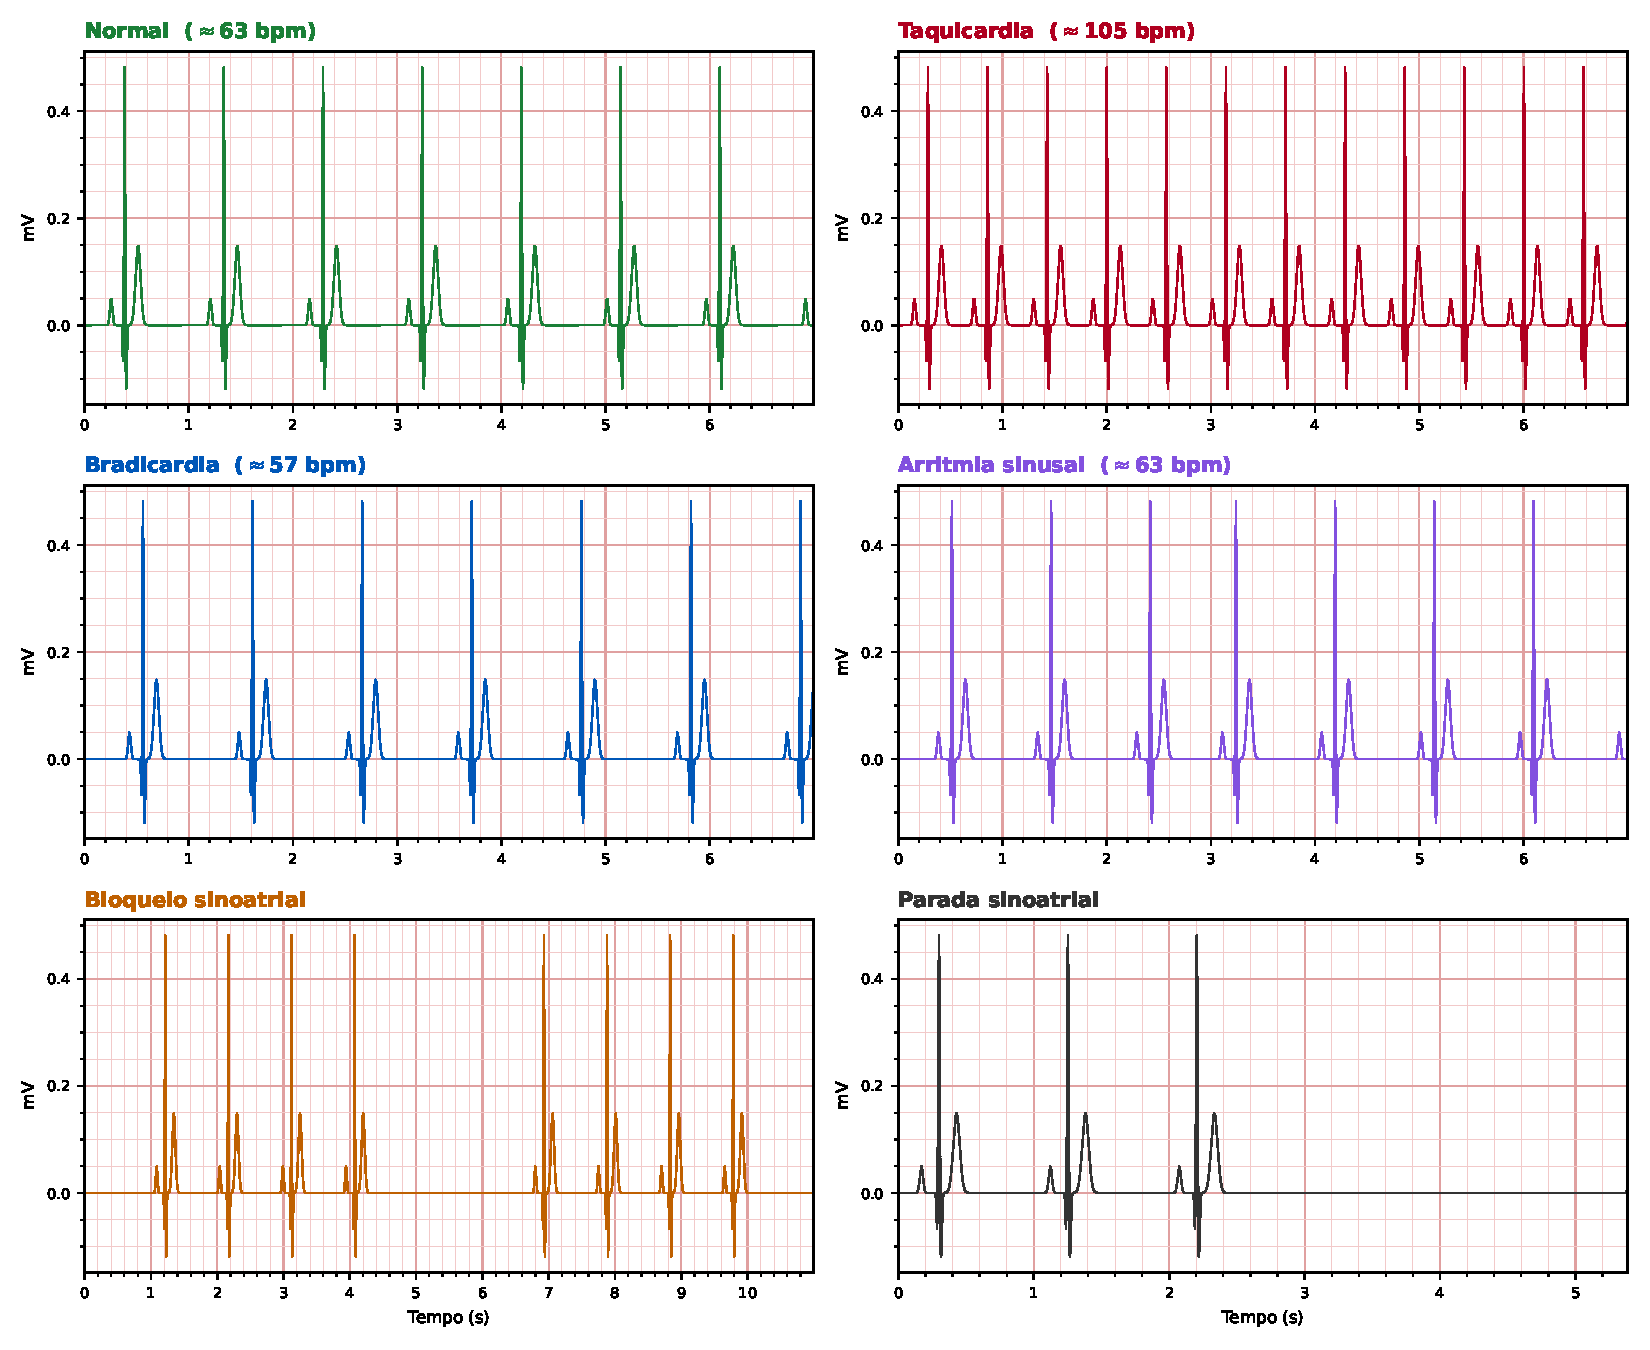
\includegraphics[width=\linewidth]{assets/casos_6classes.pdf}
\caption{Exemplos das seis classes de \acs{ECG} empregadas nos ensaios da configuração final, reproduzidos pelo gerador NI myDAQ e apresentados na escala de amplitude medida na entrada do \acs{AFE}. No painel de bloqueio a janela é centrada na pausa --- de 3,00 vezes o intervalo R-R mediano, equivalente à ausência de dois complexos QRS ---, de modo que se observe a retomada do ritmo; no de parada, a janela mostra primeiro os batimentos e termina dentro da pausa, de 3,50 vezes o intervalo mediano.}
\label{fig:casos6classes}
\end{figure}

\subsection{Desempenho sobre ECG sem ruído}
\label{sec:resFinalLimpo}

Antes de comprometer as horas de bancada, verificou-se que o binário gravado no dispositivo era de fato o que contém a sexta classe. Empregou-se, para isso, um \acs{ECG} discriminante: uma pausa de 2,2 vezes o intervalo R-R, que recai na descontinuidade identificada na Seção~\ref{sec:resZonaMorta} e que, portanto, a versão anterior classificaria como normal. A coleta retornou a máscara \texttt{0x22} --- anomalia não caracterizada acompanhada de bradicardia, esta última porque a pausa desloca a frequência média ---, confirmando a versão em execução. O procedimento é registrado por constituir a única forma de distinguir as duas versões do \textit{firmware} a partir de sua saída.

Os ensaios conduzidos sobre a configuração assim confirmada classificaram corretamente os 180 segmentos (Tabela~\ref{tab:matrizBat13}). Cada \acs{ECG} acendeu exclusivamente a sua própria \textit{flag}, e em nenhum dos 180 segmentos a sexta classe foi ativada. Esta segunda observação tem peso equivalente ao da taxa de acerto: uma classe destinada ao que não se enquadra, se disparasse sobre sinal limpo de classe conhecida, constituiria defeito, não cobertura.

\begin{table}[htb]
\centering
\caption{Matriz de confusão da configuração final sobre \acs{ECG} sem ruído (30 segmentos por classe).}
\label{tab:matrizBat13}
\resizebox{\textwidth}{!}{%
\begin{tabular}{lrrrrrrr}
\hline
\textbf{Classe do \acs{ECG}} & \textbf{Normal} & \textbf{Taqui.} & \textbf{Bradi.} & \textbf{Arritmia} & \textbf{Bloqueio} & \textbf{Parada} & \textbf{Não caract.} \\
\hline
Normal              & 30 & 0 & 0 & 0 & 0 & 0 & 0 \\
Taquicardia         & 0 & 30 & 0 & 0 & 0 & 0 & 0 \\
Bradicardia         & 0 & 0 & 30 & 0 & 0 & 0 & 0 \\
Arritmia sinusal    & 0 & 0 & 0 & 30 & 0 & 0 & 0 \\
Bloqueio sinoatrial & 0 & 0 & 0 & 0 & 30 & 0 & 0 \\
Parada sinoatrial   & 0 & 0 & 0 & 0 & 0 & 30 & 0 \\
\hline
\end{tabular}%
}
\end{table}

Valem aqui, integralmente, as ressalvas já registradas: o \acs{ECG} cedido é exatamente periódico e seus ritmos foram deliberadamente afastados dos limiares de decisão, de modo que o resultado estabelece que o sistema não erra sobre sinal controlado, e não que acerte sobre \acs{ECG} arbitrário. A medida pertinente para esta última pretensão é a da base MIT-BIH (Seção~\ref{sec:resMITBIH}).

\subsection{Desempenho sob ruído somado}
\label{sec:resFinalRuido}

As mesmas seis classes foram submetidas às três formas de ruído especificadas na
Seção~\ref{sec:resRuido}, cada uma em três amplitudes, perfazendo 54 condições e 1.620
ensaios. A taxa de acerto total foi de 92,6\,\% (1.500 de 1.620), sem qualquer erro de
processamento. A Tabela~\ref{tab:ruidoFinal} discrimina o desempenho por condição e por
classe.

\begin{table}[htb]
\centering
\caption{Desempenho da configuração final por condição de ruído (30 segmentos por classe; 180 ensaios por condição). A última coluna traz o erro absoluto médio de estimativa da frequência cardíaca.}
\label{tab:ruidoFinal}
\resizebox{\textwidth}{!}{%
\begin{tabular}{lrrrrrrrr}
\hline
\textbf{Condição} & \textbf{Normal} & \textbf{Taqui.} & \textbf{Bradi.} & \textbf{Arritmia} & \textbf{Bloqueio} & \textbf{Parada} & \textbf{Total} & \textbf{MAE FC (bpm)} \\
\hline
Deriva 0,33 Hz, 10\,\% & 30/30 & 30/30 & 30/30 & 30/30 & 30/30 & 30/30 & 180/180 & 0,2 \\
Deriva 0,33 Hz, 20\,\% & 30/30 & 30/30 & 30/30 & 30/30 & 30/30 & 30/30 & 180/180 & 0,2 \\
Deriva 0,33 Hz, 30\,\% & 30/30 & 30/30 & 30/30 & 30/30 & 30/30 & 30/30 & 180/180 & 0,2 \\
Rede 60 Hz, 10\,\%     & 30/30 & 30/30 & 30/30 & 30/30 & 30/30 & 30/30 & 180/180 & 0,2 \\
Rede 60 Hz, 20\,\%     & 30/30 & 30/30 & 30/30 & 30/30 & 30/30 & 30/30 & 180/180 & 0,3 \\
Rede 60 Hz, 30\,\%     & 0/30  & 0/30  & 0/30  & 0/30  & 30/30 & 30/30 & 60/180  & 14,1 \\
Aleatório, 10\,\%      & 30/30 & 30/30 & 30/30 & 30/30 & 30/30 & 30/30 & 180/180 & 0,2 \\
Aleatório, 20\,\%      & 30/30 & 30/30 & 30/30 & 30/30 & 30/30 & 30/30 & 180/180 & 0,2 \\
Aleatório, 30\,\%      & 30/30 & 30/30 & 30/30 & 30/30 & 30/30 & 30/30 & 180/180 & 0,2 \\
\hline
\textbf{Global}        &       &       &       &       &       &       & \textbf{1.500/1.620} & \\
\hline
\end{tabular}%
}
\end{table}

Oito das nove condições resultaram em taxa de acerto integral, com erro de estimativa da
frequência cardíaca inferior a 0,3~bpm. A deriva de linha de base foi rejeitada até a
amplitude máxima, resultado atribuível ao filtro passa-altas de 0,5~Hz, cuja frequência de
corte situa-se acima da componente de 0,33~Hz da perturbação. O ruído aleatório de banda
larga, que atravessa parcialmente a cascata de filtros e poderia produzir picos indesejados,
também não degradou o desempenho em nenhuma amplitude --- diferentemente do que se observara
sob a versão original do algoritmo (Seção~\ref{sec:resRuido}), em que a maior amplitude
custava parte dos segmentos normais.

A totalidade das 120 falhas concentra-se na interferência de rede de 60~Hz na amplitude de
30\,\%, e o modo de falha difere daquele observado sob a versão original. Sob essa condição,
as quatro classes definidas pelo ritmo foram classificadas como \textbf{bloqueio
sinoatrial}, enquanto o bloqueio e a parada permaneceram corretos. O mecanismo subjacente é o
mesmo já caracterizado --- a perda de picos R ---, mas sua consequência mudou com o critério
de pausa: um pico não localizado produz um intervalo R-R de exatamente duas vezes a mediana
do segmento, que é precisamente a definição de bloqueio na formulação relativa
(Seção~\ref{sec:resCriterioPausa}). O erro absoluto médio de estimativa da frequência
cardíaca nessa condição, de 14,1~bpm contra menos de 0,3~bpm nas demais, quantifica a
extensão da perda.

Convém estabelecer onde, na cadeia, essa perda ocorre --- questão que a taxa de acerto por si só não responde. Para dirimi-la, gravou-se no dispositivo o conteúdo do \textit{buffer} de detecção, isto é, a sequência de amostras que o algoritmo efetivamente recebeu após o divisor resistivo, o \acs{AFE} e os filtros digitais, e transferiu-se esse traçado pela interface serial (Apêndice~\ref{ap:figurasRuido}, Figura~\ref{fig:rawAdquirido}). O resultado é inequívoco: os complexos QRS encontram-se \textbf{íntegros} no sinal adquirido, com ritmo regular --- um detector de limiar simples localiza todos eles, e o intervalo R-R mediano permanece em 952~ms, idêntico ao do \acs{ECG} sem perturbação. A perda não é, portanto, da aquisição. Ela ocorre na \emph{localização} dos picos: o algoritmo de detecção reconheceu 27 dos 32 complexos presentes, e o intervalo resultante de 1.908~ms satisfez o critério de bloqueio.

A observação é coerente com o método empregado na detecção. O algoritmo reaproveitado localiza os complexos pelo método da operação de diferenças (Seção~\ref{sec:deteccaoBorda}), que opera sobre a \emph{derivada} do sinal e pareia máximos com mínimos locais. Uma interferência senoidal de 60~Hz possui derivada da mesma ordem de grandeza que a do complexo QRS, de modo que o pareamento de extremos se desorganiza e o limiar adaptativo se desloca. Corrobora essa leitura o comportamento sob ruído aleatório de idêntica amplitude, que não produz o efeito (Tabela~\ref{tab:ruidoFinal}): não é a energia da perturbação que compromete a detecção, mas sua periodicidade. Trata-se, pois, de limitação do algoritmo de detecção de picos, e não da cadeia de aquisição desenvolvida neste trabalho. Sob o critério absoluto anterior, o mesmo intervalo --- de aproximadamente 2~s, para um ritmo de 1~s --- não alcançava o piso de 4~s e não era interpretado como pausa; a versão original registrava, nessa condição, deslocamento da frequência cardíaca estimada, e não detecção de pausa. A bradicardia, que ali permanecia correta por continuar acima do limiar de 1000~ms mesmo com a frequência subestimada, passa agora a ser suprimida pela pausa indevida. O erro absoluto médio de estimativa da frequência cardíaca nessa condição, de 14,0~bpm contra menos de 0,3~bpm nas demais, quantifica a extensão da perda de picos.

Convém delimitar, por fim, o que a sexta classe de anormalidade \emph{não} resolve. Sob esta
condição ela não altera a classificação: a perda de picos é sistemática e produz intervalos
de exatamente duas vezes a mediana, que \emph{satisfazem} o critério de bloqueio. Não há, aqui,
uma lacuna entre critérios a preencher --- há um critério sendo satisfeito pela razão errada.
A classe acrescenta, ainda assim, informação ao registro: os segmentos de arritmia sinusal e
de bloqueio passam a apresentar a máscara \texttt{0x28}, registrando que, além do bloqueio
aparente, havia no segmento intervalos não enquadráveis em nenhum critério --- indício da
anomalia de aquisição que a versão anterior descartava, útil à inspeção posterior do traçado.
Os traçados das seis classes sob essa condição, o detalhe da interferência sobre o complexo
QRS e a série de intervalos R-R dela resultante são reunidos no
Apêndice~\ref{ap:figurasRuido}.

Consolidando os dois conjuntos de ensaios desta seção, registram-se 1.800 segmentos coletados, correspondentes a 15,0 horas de \acs{ECG} e a 34,6 milhões de amostras processadas, com 58.787 picos R detectados, \textbf{sem um único erro de aquisição}. O erro absoluto médio de estimativa da frequência cardíaca, excluída a condição de rede a 30\,\%, foi de 0,19~bpm sobre 1.620 segmentos.

Esses dados respondem afirmativamente à primeira das duas perguntas formuladas na Seção~\ref{sec:validacaoGerador}: a anomalia foi corretamente identificada e codificada no \textit{payload}. Em cada um dos 1.800 ensaios registrou-se, além da classe detectada, o \textit{payload} de 10 bytes montado pelo \textit{firmware}, tal como seria transmitido. Submetidos à mesma função decodificadora cadastrada no \textit{ChirpStack} (Seção~\ref{sec:resPipeline}) e confrontados campo a campo com a saída do detector, os 1.800 \textit{payloads} mostraram-se corretos --- máscara de anomalias, frequência cardíaca, intervalo R-R médio e seu desvio, contagem de picos e identificador de segmento, sem uma única divergência. A codificação do resultado da detecção, portanto, não introduz erro: o desempenho do sistema na identificação da anomalia é o da classificação, reportado nas seções anteriores, e nada se perde entre ela e a montagem do quadro a transmitir.

Quanto à segunda pergunta, o evento correto chegou ao aplicativo, conforme verificado na Seção~\ref{sec:resPipeline}. Essa verificação foi conduzida à parte dos ensaios de classificação, pela razão ali exposta: o protocolo de disparo único exige que o processamento do segmento seja iniciado por comando, o que impôs manter o enlace de rádio desativado durante os ensaios. Confrontando-se o \textit{payload} publicado com o evento persistido no banco e exibido no aplicativo, verificou-se a correspondência para as seis classes. Reconhece-se, contudo, que essa verificação tem alcance menor que a das baterias: apoia-se em seis \textit{uplinks} representativos, e não em repetição estatística. A validação conjunta do enlace de rádio com a aquisição, em regime contínuo, permanece como etapa subsequente (Capítulo~\ref{chap:conclusoes}).

Estes números caracterizam a cadeia de aquisição e de codificação desenvolvida nesta dissertação, distintamente do desempenho do algoritmo de detecção nela embarcado.

\section{Ensaios com ECG Real de Banco Público}
\label{sec:resMITBIH}

Todos os ensaios anteriores se apoiaram em \acs{ECG} gerado artificialmente e medem, por isso, o desempenho do sistema sobre morfologias e ritmos controlados. Para verificar se o desempenho observado se sustenta sobre o \acs{ECG} de pacientes reais, com toda a variabilidade fisiológica que o \acs{ECG} sintético não reproduz, recorreu-se à base MIT-BIH de arritmias — repositório público anotado por cardiologistas, de referência consolidada na literatura. Dela extraíram-se 60 segmentos de 30~s, 15 para cada uma de quatro classes — normal, taquicardia, bradicardia e arritmia sinusal —, classificadas por seus intervalos R-R. As duas classes de pausa ficaram de fora desta etapa. A seleção partiu de dezoito registros, escolhidos por cobrirem, em conjunto, as quatro classes acima, e em nenhum deles ocorre pausa na faixa exigida pelo critério de detecção. Selecionar registros pelas classes de pausa, por sua vez, não é possível de forma direta: as anotações de ritmo do MIT-BIH não preveem bloqueio nem parada sinoatrial --- o único bloqueio anotado na base é o atrioventricular de segundo grau, presente em um único registro ---, de modo que localizá-las exige varrer os intervalos R-R registro a registro. Essa varredura foi conduzida em seguida e é relatada adiante: ela recuperou o bloqueio, em um registro fora da seleção inicial, e confirmou a indisponibilidade da parada sinoatrial.

\subsection{Desempenho do algoritmo isolado}
\label{sec:resMitbihAlgoritmo}

Numa primeira etapa, os 60 segmentos foram fornecidos diretamente ao algoritmo de detecção, sem passar pela cadeia de aquisição, de modo a medir o \emph{algoritmo} isoladamente sobre o sinal real. A taxa de acerto total foi de 81,7\,\% (49 dos 60 segmentos), com a matriz de confusão da Tabela~\ref{tab:matrizMITBIH}. A queda em relação aos 100\,\% dos ensaios com \acs{ECG} controlado concentra-se, quase integralmente, no critério de arritmia sinusal: das onze classificações incorretas, dez são detecções de arritmia sobre segmentos de outras classes, e seu valor preditivo positivo cai a 58\,\%. Trata-se da mesma baixa especificidade caracterizada na Seção~\ref{sec:resArritmia}, agora manifesta sobre \acs{ECG} real: a variabilidade batimento a batimento naturalmente presente no ritmo de pacientes reais satisfaz o critério de arritmia sinusal, ausente do \acs{ECG} sintético regular. Esse valor de 81,7\,\% representa, assim, o teto do \emph{método} sobre sinal real, e não uma limitação introduzida pelo sistema aqui desenvolvido.

\begin{table}[htb]
\centering
\caption{Matriz de confusão sobre o \acs{ECG} real (60 segmentos do MIT-BIH, 15 por classe, fornecidos diretamente ao detector; linha = classe esperada, coluna = classe detectada).}
\label{tab:matrizMITBIH}
\begin{tabular}{l c c c c}
\hline
\textbf{Esperada / Detectada} & \textbf{Normal} & \textbf{Taqui.} & \textbf{Bradi.} & \textbf{Arrit.} \\
\hline
Normal            & 11 & 0  & 0  & 4  \\
Taquicardia       & 0  & 11 & 0  & 4  \\
Bradicardia       & 0  & 0  & 13 & 2  \\
Arritmia sinusal  & 0  & 1  & 0  & 14 \\
\hline
\end{tabular}
\end{table}

\subsection{Desempenho da cadeia completa}
\label{sec:resMitbihCadeia}

Numa segunda etapa, os mesmos segmentos do MIT-BIH foram reproduzidos pelo gerador e adquiridos pela cadeia de aquisição completa — divisor resistivo, \acs{AFE}, filtros digitais e quantização a 640~SPS —, no mesmo protocolo de disparo único das baterias anteriores. Acrescentou-se, nesta etapa, uma quinta classe. A varredura por pausas anunciada acima, estendida a registros fora da seleção inicial, localizou o registro~232. Trata-se de registro anotado como bradicardia sinusal --- manifestação da disfunção do nó sinusal, que é precisamente o quadro que produz o bloqueio sinoatrial ---, e nele há catorze pausas na faixa, agrupadas de modo a haver janelas de 30~s contendo mais de uma, condição que o critério exige. Dele extraíram-se os dois segmentos de bloqueio empregados nesta bateria. A parada sinusal permaneceu indisponível: os únicos intervalos superiores a seis segundos, entre os vinte registros varridos, ocorrem no registro~207, dentro de episódios de \textit{flutter} ventricular em que os batimentos não recebem marcação --- o intervalo é artefato de anotação, e não pausa sinusal, de modo que empregá-lo seria incorreto. Os representantes de cada classe foram escolhidos entre os segmentos que o detector já classificava corretamente na etapa anterior, maximizando a distância ao limiar de decisão, e cada um foi reproduzido 30 vezes, perfazendo 150 ensaios. O sistema classificou corretamente os 150, sem erro de processamento.

O valor dessa etapa não está no número em si — a seleção de representantes favoráveis o torna deliberadamente otimista e ele não deve ser lido como taxa de acerto do sistema sobre \acs{ECG} real qualquer —, mas na comparação \emph{pareada} com a primeira etapa. Como o conjunto de \acs{ECG} é o mesmo, a diferença entre as duas mede exclusivamente o que a aquisição acrescenta: nos segmentos em que o algoritmo decide corretamente sobre o sinal ideal, a cadeia de aquisição preserva a decisão integralmente, sem que o divisor, o \acs{AFE}, os filtros ou a quantização custem um único acerto. As duas etapas, em conjunto, separam a limitação do \emph{método} (os 81,7\,\% da sexta) do custo da \emph{aquisição} (nulo, pela oitava) — atribuição que nenhuma das duas, isolada, permitiria.

\subsection{Efeito das revisões do critério sobre o ECG real}
\label{sec:resMitbihConfig}

Os valores das duas etapas referem-se ao critério de pausa por duração absoluta, vigente quando foram medidas. Como a revisão desse critério altera a regra de decisão, os 60 segmentos foram reavaliados sobre as configurações posteriores do detector, e o resultado é reportado na Tabela~\ref{tab:mitbihConfig}. A formulação relativa, isoladamente, reduz a taxa de acerto a 71,7\,\%: em ritmos intrinsecamente irregulares --- fibrilação atrial e ectopia ventricular frequente, presentes nos registros 200, 202 e 203 --- a mediana deixa de representar um ritmo de base, e sete segmentos passam a satisfazer o critério de pausa sem que haja pausa sinusal. O mecanismo é o mesmo identificado na Seção~\ref{sec:resFinalRuido}: intervalos R-R longos, aqui de origem fisiológica e não de perda de picos, satisfazem a razão exigida. Com a sexta classe de anormalidade descrita na Seção~\ref{sec:resNaoCaracterizada}, que reclassifica essas pausas em vez de afirmá-las, a taxa de acerto alcança 85,0\,\%, superando o valor da configuração original.

\begin{table}[htb]
\centering
\caption{Taxa de acerto sobre os 60 segmentos do MIT-BIH nas configurações do critério de detecção. $^{\dagger}$ Configuração avaliada apenas sobre esta base, sem ensaio em bancada.}
\label{tab:mitbihConfig}
% Terceira coluna em p{}: com especificador `l` o texto não quebra e a tabela
% ultrapassa a margem da página.
\begin{tabular}{@{}l c p{6.2cm}@{}}
\hline
\textbf{Configuração do critério} & \textbf{Taxa de acerto total (\%)} & \textbf{Limitação dominante} \\
\hline
Pausa por duração absoluta    & 81,7 & Especificidade da arritmia sinusal \\
Pausa relativa ao R-R         & 71,7 & Falso positivo de pausa em ritmo irregular \\
Pausa relativa + sexta classe & 85,0 & Especificidade da arritmia sinusal \\
Limiar de ritmo pela mediana$^{\dagger}$ & 90,0 & Especificidade da arritmia sinusal \\
\hline
\end{tabular}
\end{table}


Cabe registrar, por último, uma melhoria identificada depois de concluídos os ensaios de bancada e
avaliada apenas sobre esta base, sem passar pela bancada. O critério de pausa compara a
duração do intervalo com a mediana do segmento, mas os limiares de taquicardia e de
bradicardia continuavam a ser aplicados ao intervalo R-R \emph{médio}. A diferença é
irrelevante em ritmo regular, em que média e mediana coincidem, mas não quando há pausa: um
único intervalo longo desloca a média e pode rotular como bradicardia um segmento cujo ritmo
de base é normal. Aplicando-se os dois limiares à mediana, a taxa de acerto sobre os 60
segmentos desta base passa de 85,0\,\% para 90,0\,\%, com três segmentos corrigidos e nenhum
prejudicado --- todos em registros de ritmo intrinsecamente irregular, onde a média é menos
representativa. A alteração não foi incorporada aos ensaios relatados neste capítulo, que
medem a configuração de \textit{firmware} efetivamente ensaiada em bancada; ela é registrada
aqui como aprimoramento medido e verificável, cuja validação sobre a cadeia completa fica
para etapa subsequente (Capítulo~\ref{chap:conclusoes}).


\section{Validação do Fluxo de Dados de Ponta a Ponta}
\label{sec:resPipeline}

A integração entre a infraestrutura de rede e a camada de aplicação foi validada de forma independente da aquisição do biopotencial. Utilizando uma ferramenta de publicação \acs{MQTT} para simular \textit{uplinks} do \textit{ChirpStack}, verificou-se que o serviço de ingestão (Seção~\ref{sec:ingestor}) decodificou corretamente o \textit{payload}, identificou o dispositivo pelo seu \textit{DevEUI}, gravou o evento cardíaco na coleção correspondente do \textit{Firestore} e, nos casos críticos, registrou as notificações destinadas aos profissionais de saúde. As alterações no banco propagaram-se, em tempo real, para o aplicativo móvel por meio do mecanismo de \textit{listeners} do \textit{Firestore}, confirmando o funcionamento do caminho completo de dados: dispositivo, \textit{LoRaWAN}, \textit{ChirpStack}, \acs{MQTT}, \textit{ingestor}, \textit{Firestore} e aplicativo.

Cada \textit{uplink} carregou o \textit{payload} de 10 bytes definido na Seção~\ref{sec:resTransmissao} (Tabela~\ref{tab:payload}), no qual o primeiro byte codifica, como máscara de bits, as anomalias detectadas e os demais transportam a frequência cardíaca média e campos auxiliares de contexto. Na recepção, a função decodificadora (\textit{codec}) cadastrada no \textit{ChirpStack} (Figura~\ref{fig:decoder}) reconstrói esses campos e os disponibiliza em \texttt{data.object}; a partir deles, o serviço de ingestão deriva o tipo de evento segundo uma ordem de precedência, do achado de maior para o de menor risco: parada, bloqueio, taquicardia, bradicardia, arritmia sinusal e anomalia não caracterizada, preservando no registro a máscara completa com todas as anomalias do segmento. Essa ordem não reproduz uma taxonomia normativa --- não se identificou, na literatura consultada, prioridade estabelecida para o colapso de achados simultâneos em um único rótulo ---, mas constitui decisão de projeto, ordenada pelo risco potencial de cada condição: as pausas sinusais podem evoluir para comprometimento hemodinâmico, ao passo que a arritmia sinusal é fisiológica em repouso. Seu efeito restringe-se ao rótulo exibido, uma vez que a máscara é preservada no registro e é sobre ela que operam os contadores de alarme (Seção~\ref{sec:appFunc}). A arritmia sinusal ocupa a menor prioridade por ser muitas vezes uma alteração normal causada pela respiração, como será detalhado posteriormente na (Seção~\ref{sec:resArritmia}): como sua detecção frequentemente acompanha outras detecções, mantê-la à frente mascararia eventos críticos como a taquicardia; assim, um segmento só é classificado como arritmia quando essa é a única anomalia detectada. A precedência decide, contudo, apenas o rótulo do evento: a confirmação de alarme no aplicativo (Seção~\ref{sec:appFunc}) opera sobre a máscara preservada no registro, de modo que uma arritmia sinusal detectada em conjunto com outra anomalia continua a incrementar o seu próprio contador, ainda que o evento receba o rótulo da classe mais grave. Descartar a coocorrência seria inseguro: a informação de contexto que a arritmia carrega deixaria de existir justamente nos segmentos em que há mais de uma alteração.

A validação empregou seis \textit{payloads} representativos, um para cada classe de evento, publicados no tópico de \textit{uplink} por meio de uma ferramenta de simulação. Cada caso foi publicado 30 vezes, perfazendo 180 \textit{uplinks}: uma única publicação por classe verificaria apenas a decodificação, ao passo que a repetição permite observar se o serviço deixa de processar mensagens sob publicações sucessivas. Em todas as 180, o serviço de ingestão decodificou os campos, derivou corretamente o tipo de evento e a frequência cardíaca, e persistiu o registro na coleção de eventos cardíacos do \textit{Firestore}, sem perda nem duplicação, conforme a Tabela~\ref{tab:casosPipeline}. Os eventos propagaram-se, em tempo real, para o painel de monitoramento do aplicativo (Figura~\ref{fig:telasApp}a).

\begin{table}[htb]
\centering
\caption{Casos publicados na validação do fluxo de ponta a ponta e o respectivo evento persistido no \textit{Firestore}. Cada caso foi publicado 30 vezes; todas as 180 publicações resultaram em registro gravado.}
\label{tab:casosPipeline}
\begin{tabular}{l c c c l c}
\hline
\textbf{Caso} & \textbf{\textit{flags}} & \textbf{BPM} & \textbf{Publicações} & \textbf{Evento gravado} & \textbf{Crítico} \\
\hline
Normal        & \texttt{0x00} & 72  & 30 & NORMAL       & Não \\
Taquicardia   & \texttt{0x01} & 120 & 30 & TAQUICARDIA  & Sim \\
Bradicardia   & \texttt{0x02} & 48  & 30 & BRADICARDIA  & Sim \\
Arritmia      & \texttt{0x04} & 82  & 30 & ARRITMIA     & Sim \\
Bloqueio      & \texttt{0x08} & 50  & 30 & BLOQUEIO     & Sim \\
Parada        & \texttt{0x10} & 56  & 30 & PARADA       & Sim \\
\hline
\textbf{Total} & & & \textbf{180} & & \\
\hline
\end{tabular}
\end{table}

A consistência dos dados foi conferida confrontando os registros armazenados localmente no dispositivo, obtidos por meio dos comandos de despejo pela interface serial, com os eventos persistidos no banco em nuvem, não se observando divergências nos campos transmitidos.
\section{Verificação do Aplicativo Móvel}
\label{sec:resApp}

O aplicativo foi compilado para \textit{Android} pelo serviço de compilação em nuvem da plataforma \textit{Expo} e instalado em um aparelho físico, de onde provêm as telas desta seção. A verificação incidiu sobre o que a descrição funcional (Seção~\ref{sec:appFunc}) não determina: o comportamento da interface diante dos eventos efetivamente produzidos pela cadeia de aquisição e transmissão.

O painel de eventos cardíacos foi observado durante as publicações relatadas na Seção~\ref{sec:resPipeline}. Os eventos apareceram na lista sem qualquer recarga manual, identificados pelo tipo de anomalia, pela frequência cardíaca, pelo paciente associado e pelo horário de registro, com realce cromático proporcional à gravidade (Figura~\ref{fig:telasApp}a). A correspondência entre o que foi publicado e o que a tela exibiu --- inclusive nos valores de frequência cardíaca de cada classe --- fecha a cadeia do dispositivo à interface. Como a leitura é feita diretamente no banco em nuvem, sem \acs{API} intermediária, o aplicativo não depende da rede local em que operam o \textit{gateway} e o serviço de ingestão.

As demais telas foram exercitadas com dados do ambiente de validação (Figura~\ref{fig:telasApp}b--f): cadastro e consulta de pacientes, vínculo e desvínculo de dispositivos, ativação de profissionais pendentes e gestão de instituições. O controle de acesso por perfil e por estado de vínculo é exercido pelas regras de segurança do \textit{Firestore} (Seção~\ref{sec:seguranca}), e não pela interface, de modo que a restrição não depende do cliente.

Duas verificações ficaram fora do alcance desta etapa: a avaliação de usabilidade com os profissionais de saúde e o ensaio com vários dispositivos transmitindo ao mesmo tempo. Ambas dependem do uso em ambiente clínico, previsto como etapa futura.

\begin{figure}[htbp]
\centering
\subfloat[Painel de eventos cardíacos]{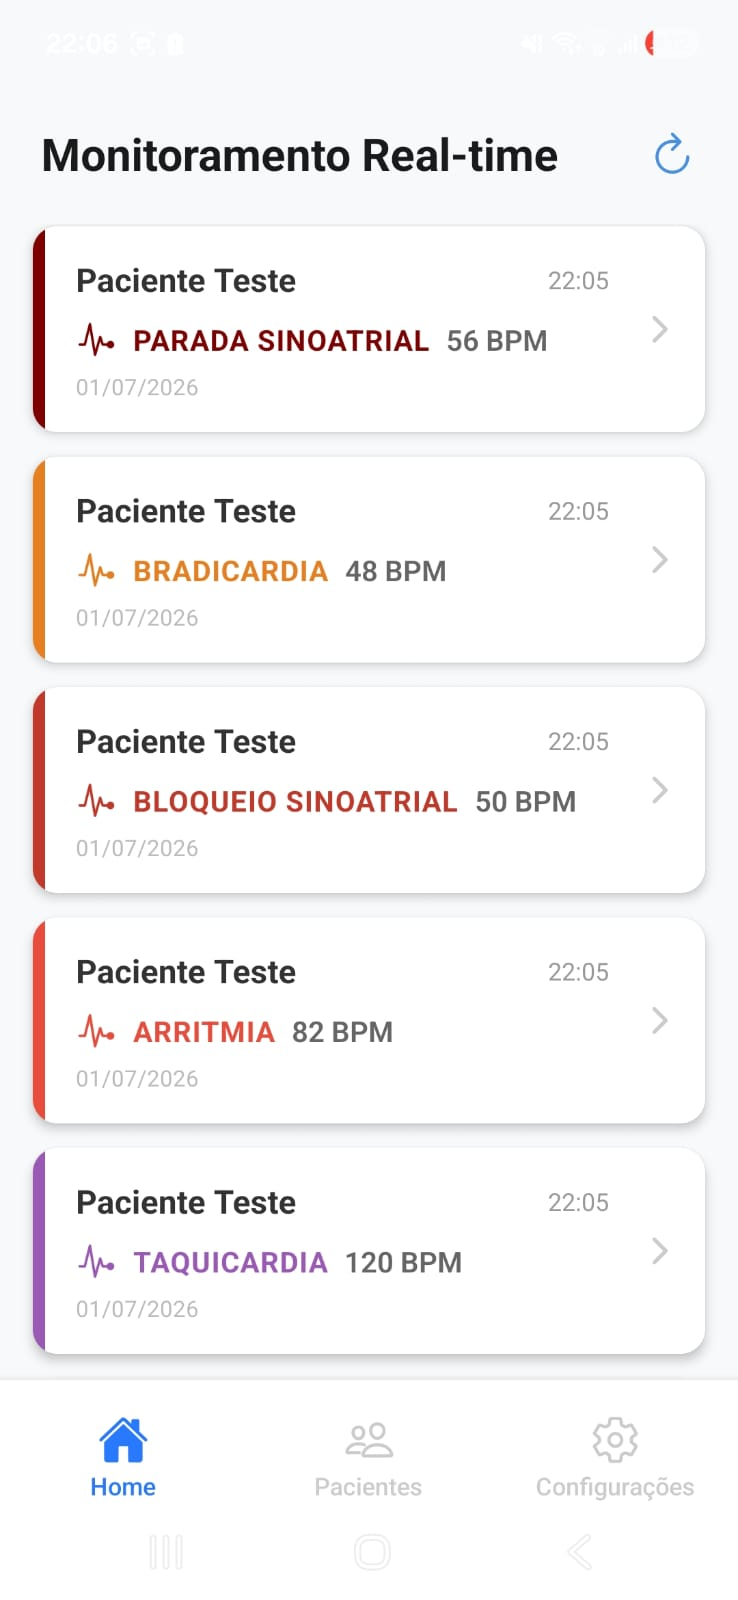
\includegraphics[width=0.30\linewidth]{assets/telaMonitoramento.jpeg}}\hfill
\subfloat[Pacientes]{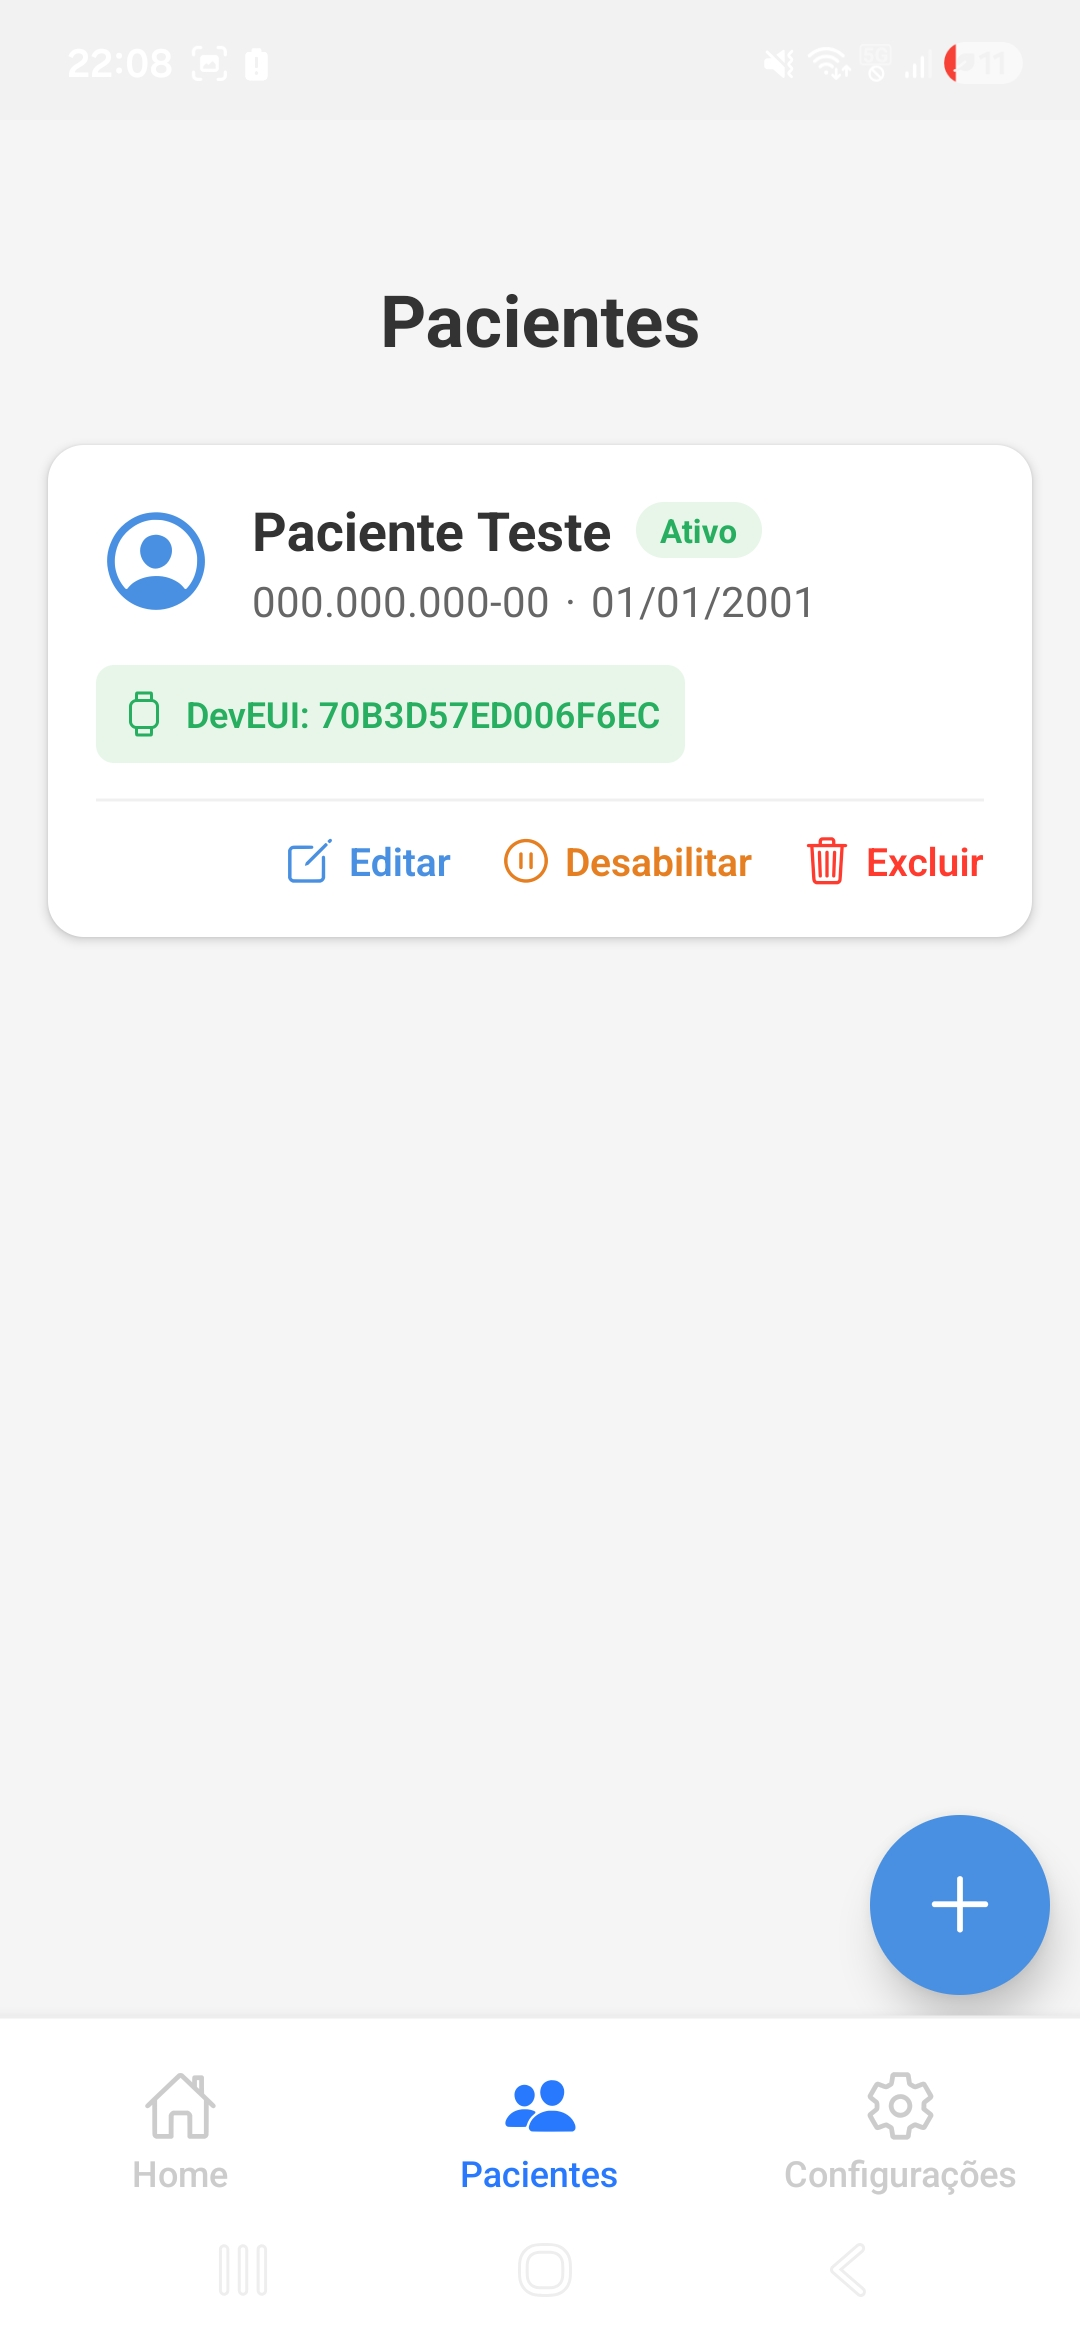
\includegraphics[width=0.30\linewidth]{assets/telaPacientes.jpeg}}\hfill
\subfloat[Dispositivos]{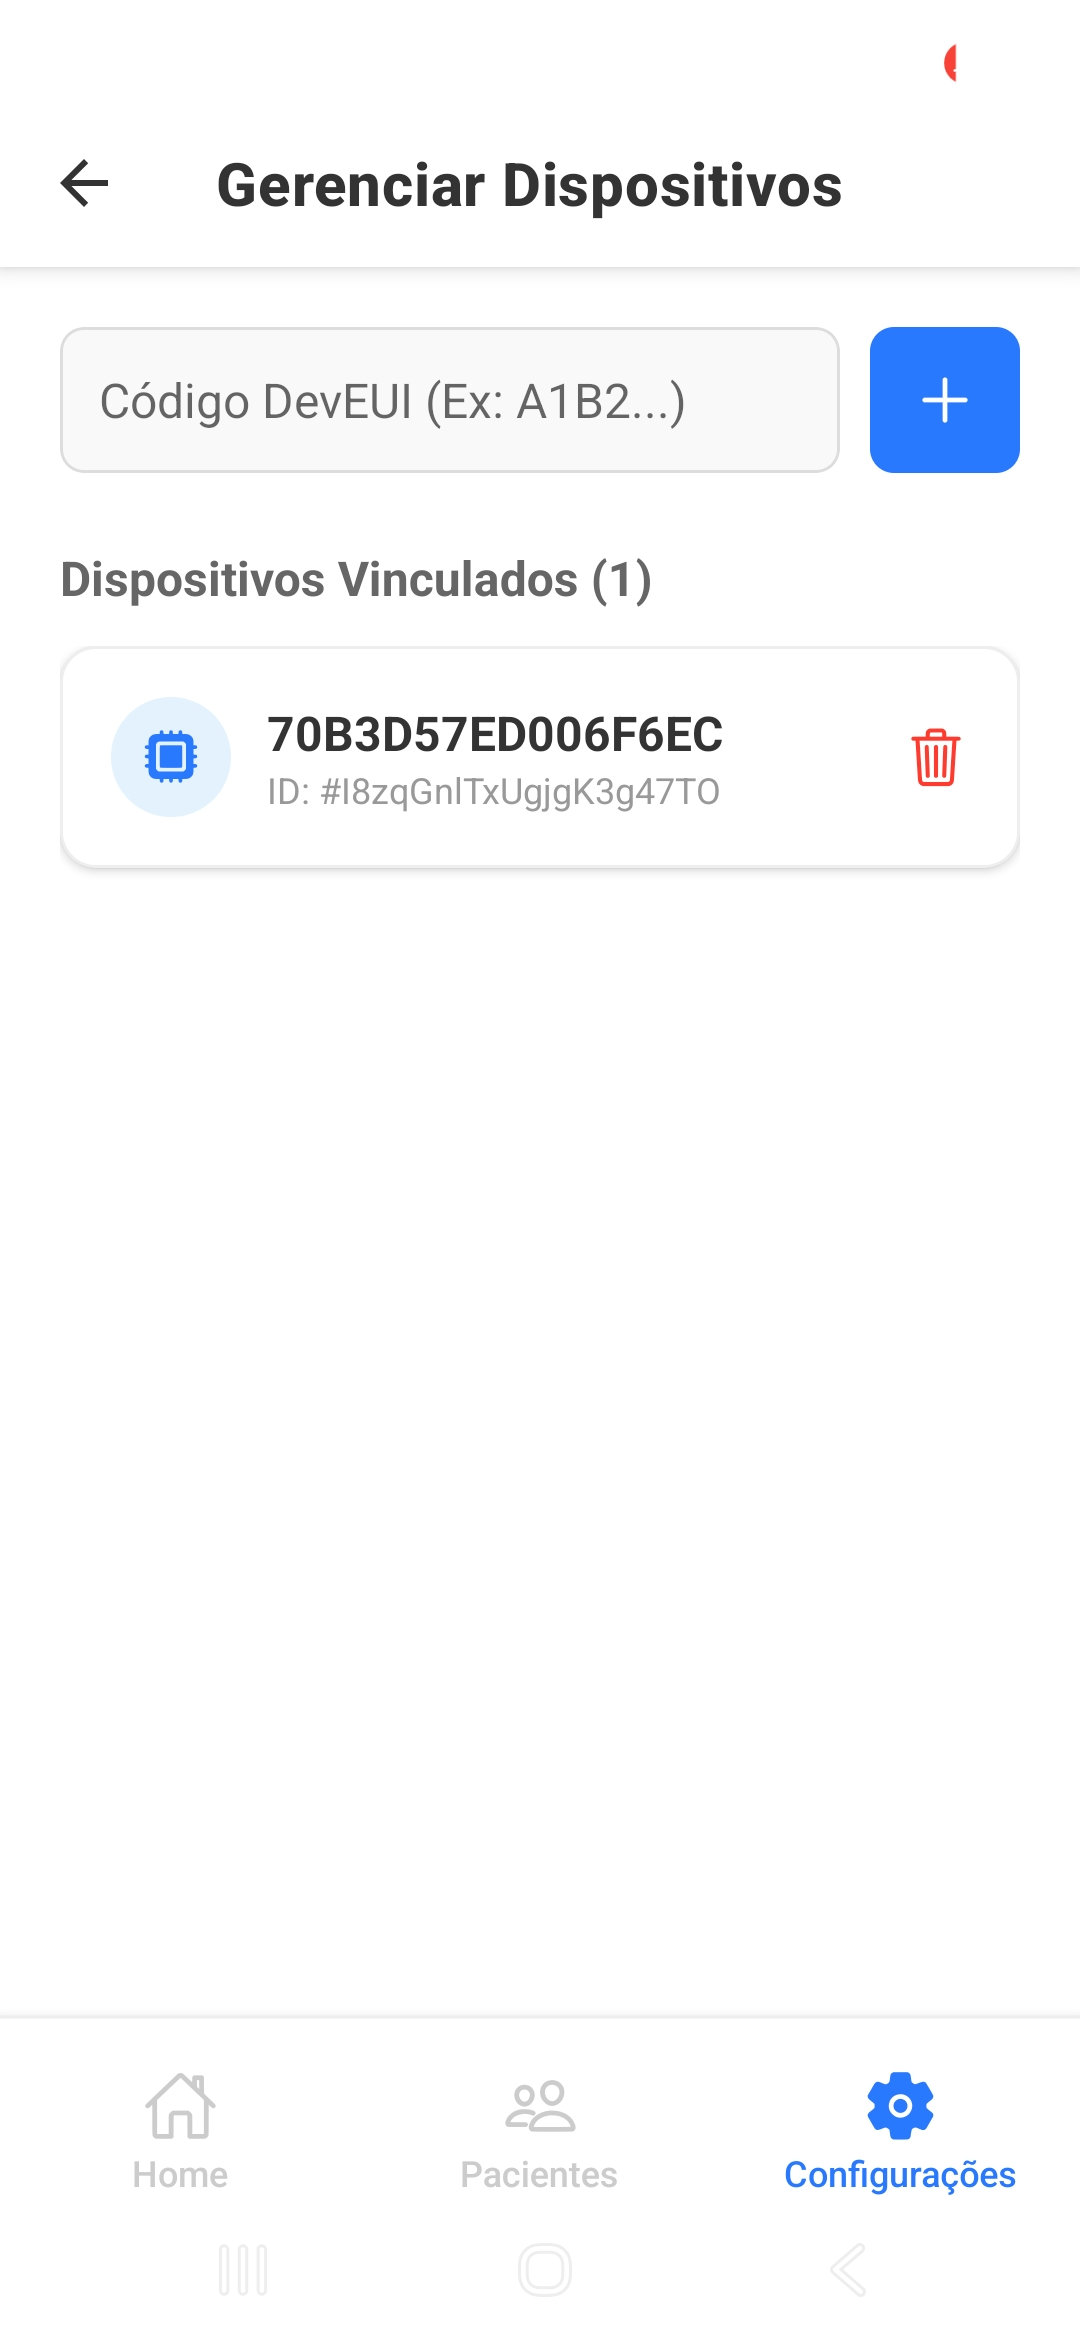
\includegraphics[width=0.30\linewidth]{assets/telaDispositivos.jpeg}}\\[1ex]
\subfloat[Usuários]{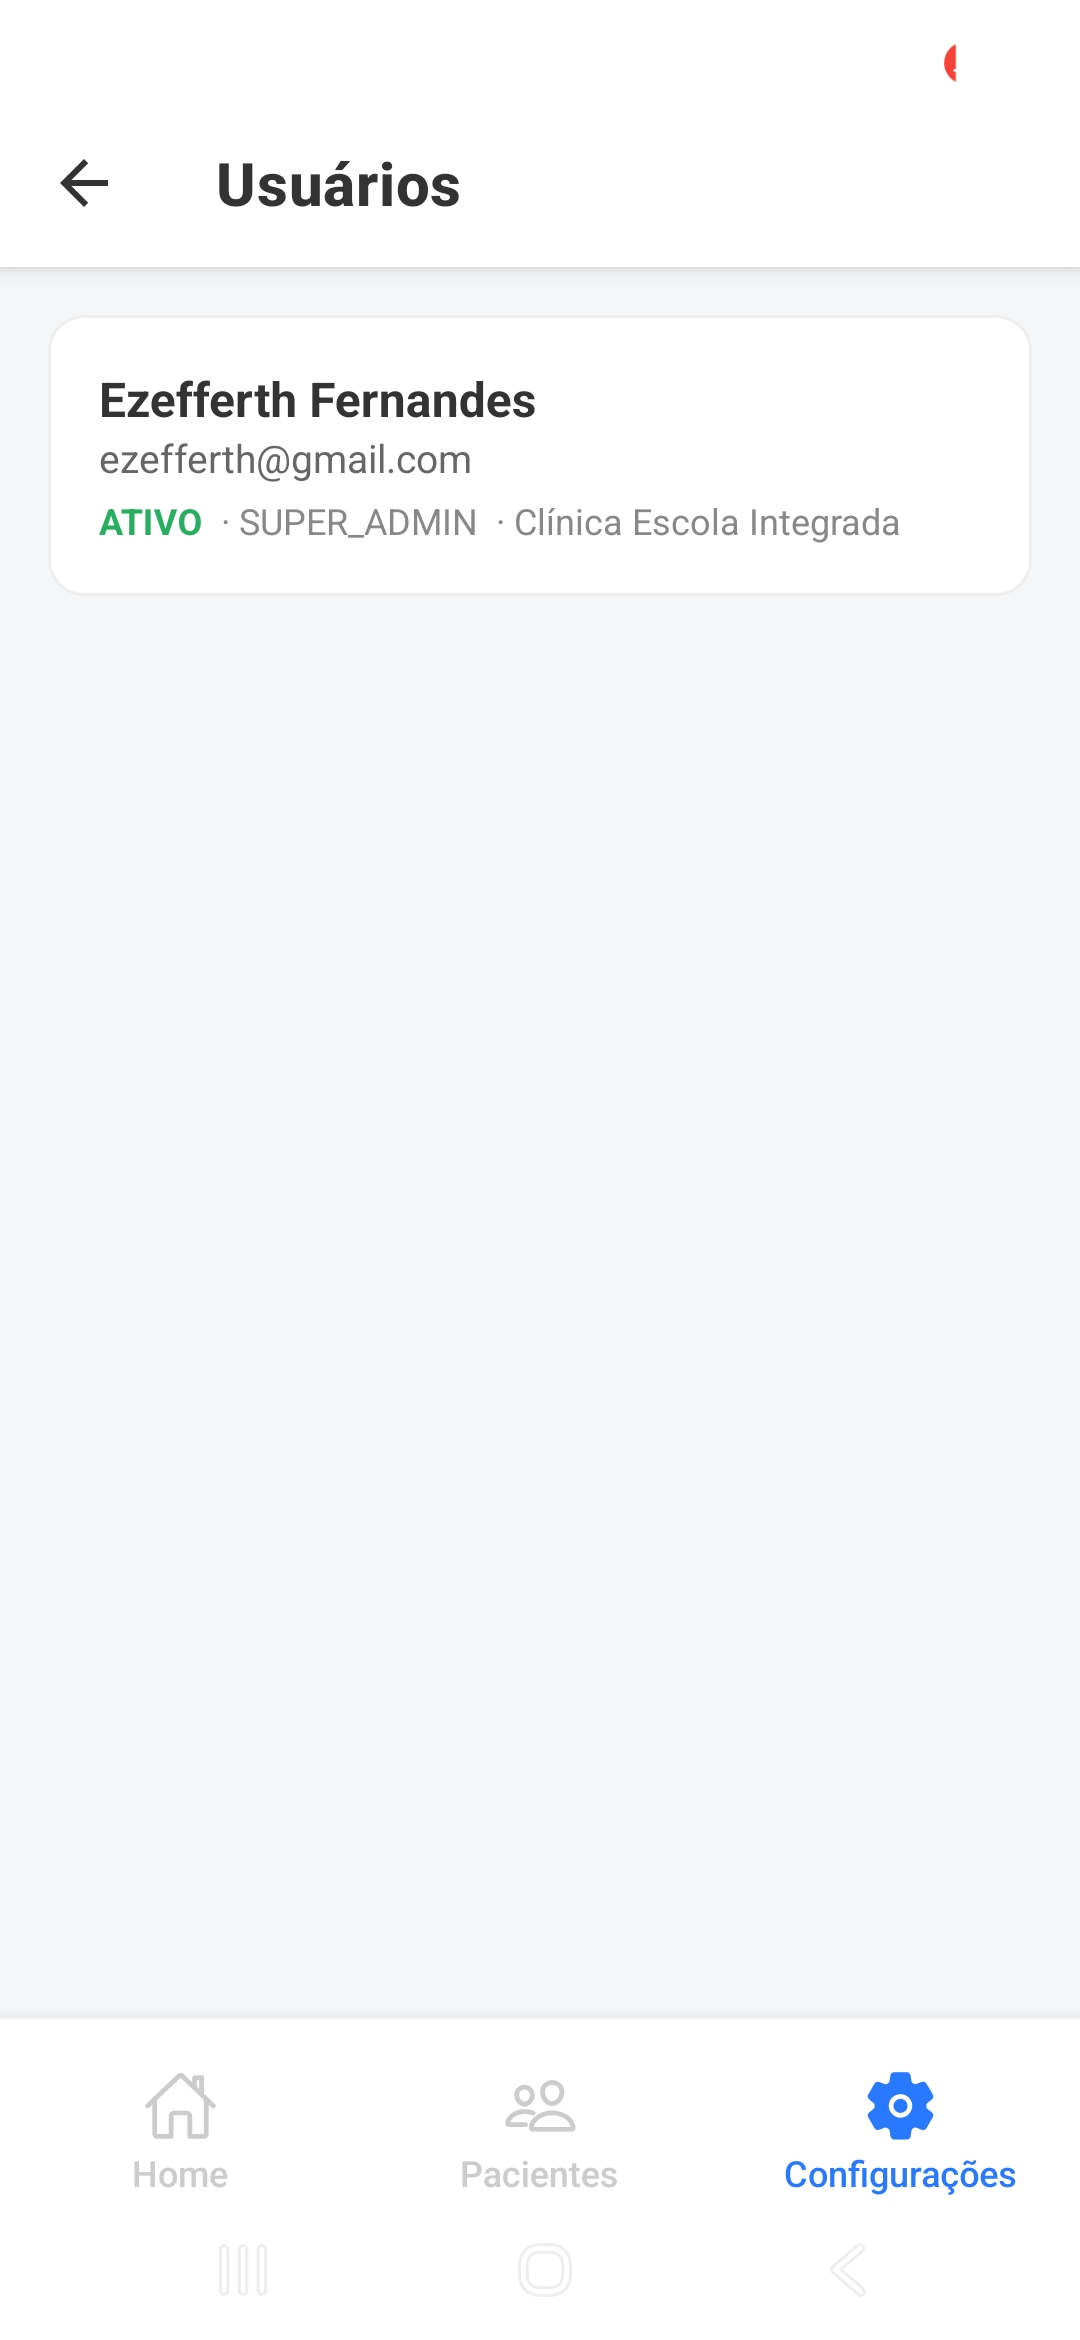
\includegraphics[width=0.30\linewidth]{assets/telaUsuarios.jpeg}}\hfill
\subfloat[Instituições]{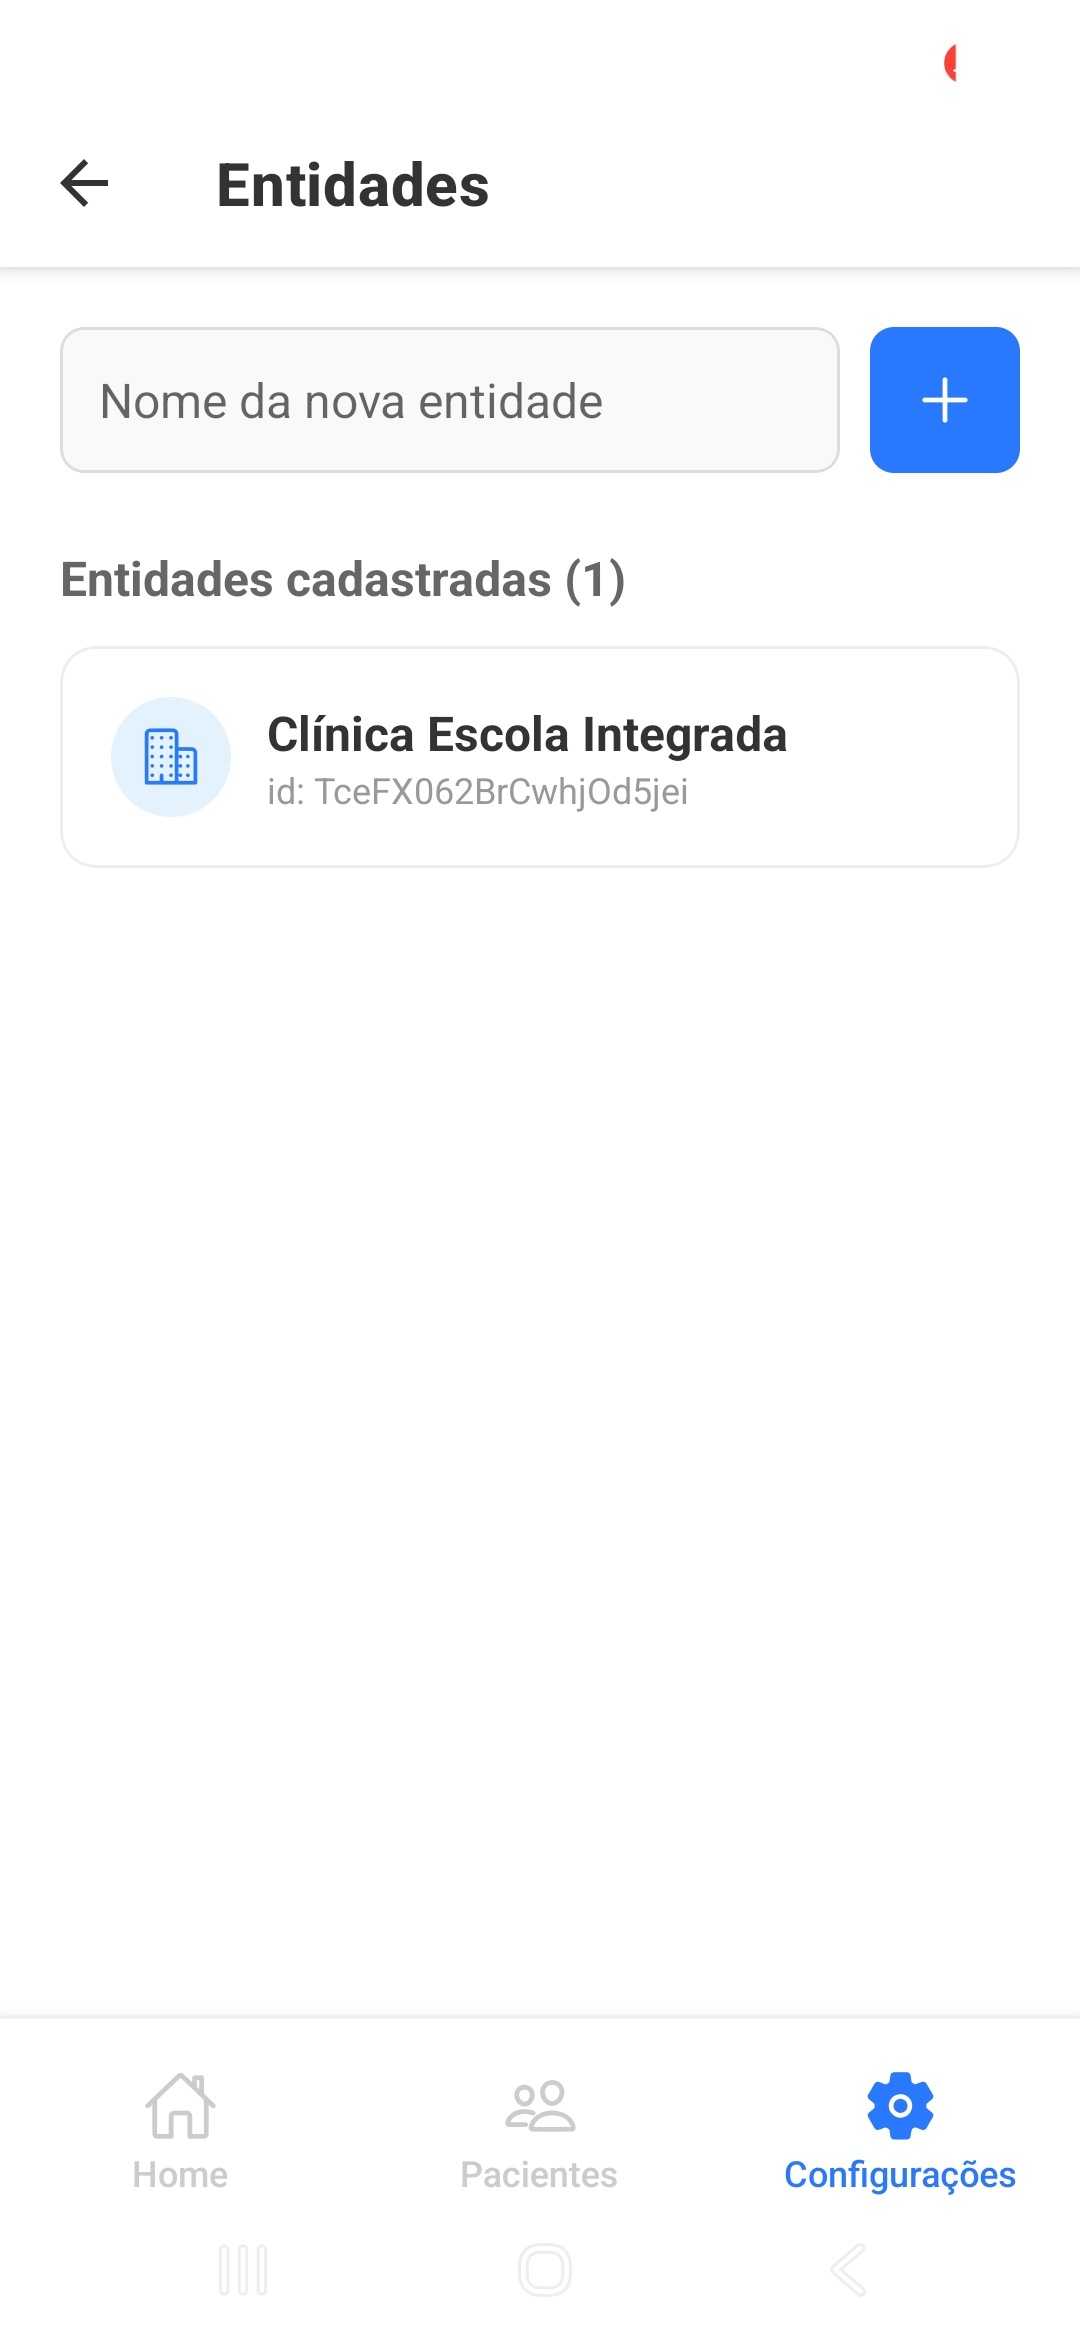
\includegraphics[width=0.30\linewidth]{assets/telaEntidades.jpeg}}\hfill
\subfloat[Configurações]{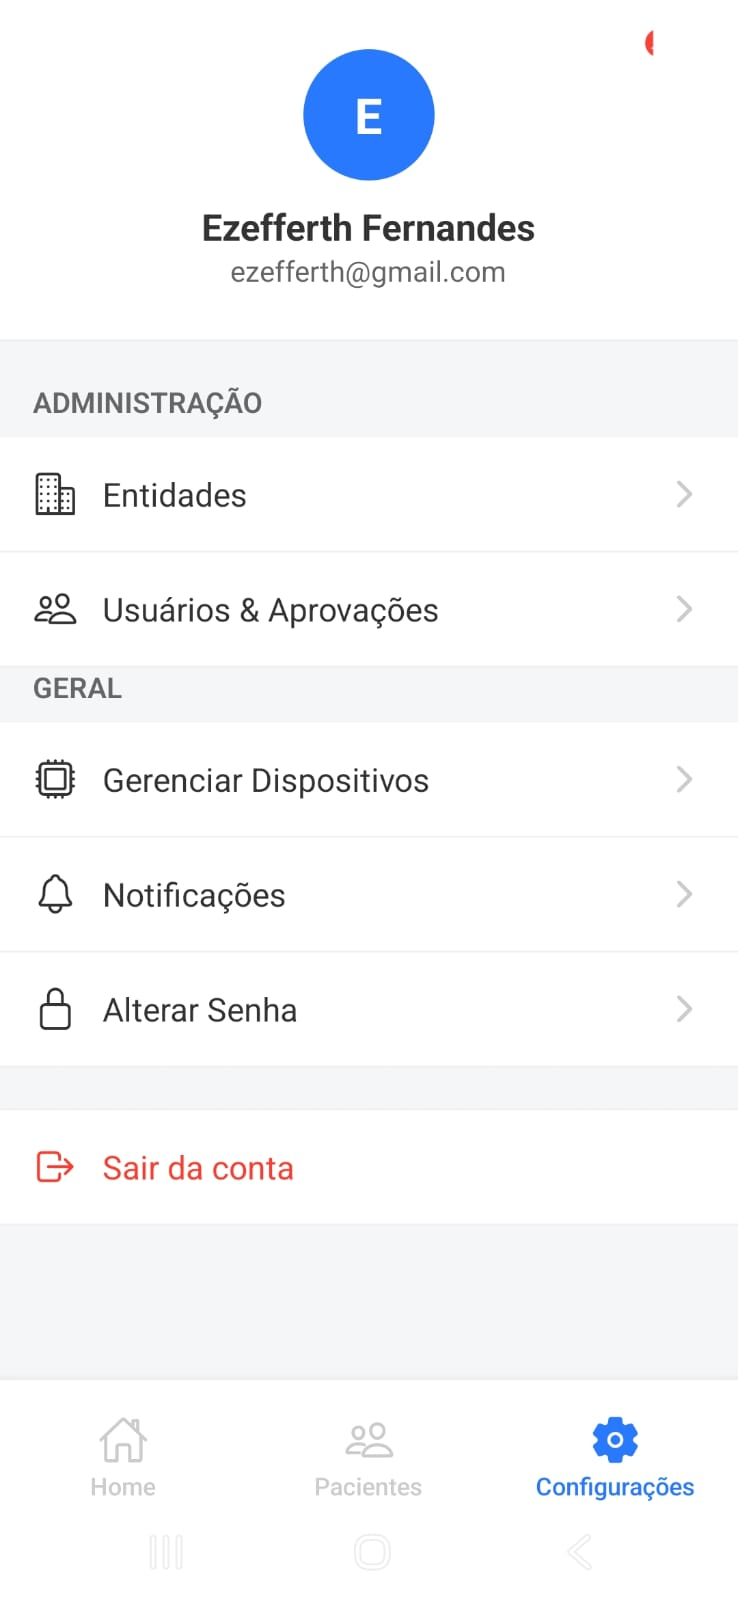
\includegraphics[width=0.30\linewidth]{assets/telaConfiguracoes.jpeg}}
\caption{Telas principais do aplicativo móvel: (a) painel de eventos cardíacos em tempo real, (b) gestão de pacientes, (c) gestão de dispositivos, (d) gestão de usuários, (e) gestão de instituições e (f) configurações.}
\label{fig:telasApp}
\end{figure}

\section{Detecção na Borda e Redução do Payload}
\label{sec:resDeteccao}

A estratégia de detecção na borda foi verificada quanto ao seu efeito sobre o volume de dados transmitidos. Enquanto a transmissão da forma de onda completa de um segmento de 30~s, à taxa efetiva de 640 SPS e 2 bytes por amostra, exigiria o envio de 38.400 bytes, o resumo produzido pelo algoritmo embarcado ocupou apenas 10 bytes por segmento — uma redução de mais de três ordens de grandeza. Esse \textit{payload} compacto é transmitido em um único \textit{uplink} a cada 30~s, com tempo de ocupação do canal (\textit{Time on Air}) reduzido e amplo respeito às restrições de \textit{duty cycle}, ao contrário da transmissão fragmentada da forma de onda, cujo tempo total inviabilizava o monitoramento contínuo (Seção~\ref{sec:resTransmissao}).

Essa abordagem é coerente com a análise de viabilidade da literatura, segundo a qual o \textit{LoRaWAN} é adequado à transmissão de alertas de detecção e de parâmetros vitais, porém não à da forma de onda contínua \citep{lorawanWaveform}. A preservação local da forma de onda dos segmentos anormais (Seção~\ref{sec:armazenamento}) manteve a possibilidade de análise detalhada \textit{a posteriori}, sem onerar o canal.
\section{Considerações sobre os Resultados}
\label{sec:resConsideracoes}

Os resultados validaram as decisões estruturais do projeto. Consolidou-se a infraestrutura
\textit{LoRaWAN} com servidor de rede local; determinou-se a taxa de amostragem efetiva do
conversor, divergente da documentada pela biblioteca de controle; corrigiu-se a aquisição do
biopotencial pela reconfiguração da referência de modo comum, obtendo-se um traçado com
morfologia adequada e ruído de rede atenuado; verificou-se a integração de ponta a ponta
entre o dispositivo, a nuvem e o aplicativo; e confirmou-se que a detecção na borda viabiliza
a operação do sistema sobre \textit{LoRaWAN}, cuja capacidade não admite a transmissão da
forma de onda.

As cinco etapas de ensaio cumpriram funções distintas, e é o conjunto delas, não qualquer uma
isolada, que sustenta as conclusões. O \acs{ECG} registrado no próprio autor
(Seção~\ref{sec:resEcgProprio}) revelou os dois defeitos de aquisição corrigidos no trabalho
--- a saturação do enlace serial e a perda periódica de amostras por bloqueio do laço --- e a
baixa especificidade do critério de arritmia sinusal em repouso. O \acs{ECG} sintetizado neste
trabalho (Seção~\ref{sec:resEcgSintetico}) estabeleceu o limite superior do desempenho, sob
ritmo controlado, e permitiu medir o erro de estimativa da frequência cardíaca na presença de
variabilidade: entre 0,2 e 0,5~bpm. O \acs{ECG} cedido pelo orientador, sob a versão original
do algoritmo (Seção~\ref{sec:resEcgOrientadorOriginal}), expôs as limitações da regra de
decisão --- em especial a definição de pausa por duração absoluta, que obrigava a adaptar o
material de teste à regra em vez de reconhecer o quadro clínico --- e a degradação sob
interferência de rede de forte amplitude. O mesmo \acs{ECG}, sob a versão final
(Seção~\ref{sec:resEcgOrientadorFinal}), mediu o efeito das revisões em condições idênticas:
classificação correta dos 180 segmentos sobre sinal sem ruído e 92,6\,\% sob as 54 condições
de ruído, com as falhas inteiramente concentradas em uma condição conhecida e diagnosticada. O
\acs{ECG} real da base MIT-BIH (Seção~\ref{sec:resMITBIH}), por fim, mediu o que nenhum sinal
sintético mede: o comportamento do método diante da variabilidade fisiológica de pacientes
reais.

Convém distinguir, nessa leitura, o que se mede sobre o \emph{algoritmo} reaproveitado do que
se mede sobre a \emph{cadeia} desenvolvida nesta dissertação. Quanto ao algoritmo, o
desempenho apresenta-se em três níveis, e é a gradação entre eles que o caracteriza: sobre
\acs{ECG} de classe conhecida e ritmo controlado não há erro de classificação; sobre \acs{ECG}
humano real, a taxa de acerto é de 85,0\,\%, limitada sobretudo pela especificidade do
critério de arritmia sinusal; e sob interferência de rede em amplitude severa o sistema falha
de modo conhecido, por perda de picos na etapa de localização dos complexos. Quanto à cadeia,
as 1.800 aquisições dos dois conjuntos de ensaios finais --- 15 horas de sinal, 34,6 milhões de amostras
--- transcorreram sem erro de aquisição, sem perda de segmento e sem uma única divergência na
montagem do \textit{payload}, com erro médio de estimativa da frequência cardíaca de
0,19~bpm. É esta última medida que responde ao objetivo desta dissertação; a primeira
caracteriza o detector reaproveitado, cuja revisão, conduzida sob orientação de seus autores,
elevou o desempenho sobre \acs{ECG} real acima do valor da formulação original.

Três limitações delimitam o alcance do que se mediu. Todo o \acs{ECG} de classe conhecida
empregado é sintético, e ainda que reproduzido fisicamente e adquirido pela cadeia completa,
não reproduz a variabilidade de morfologia de um paciente em atividade física. A única
avaliação sobre \acs{ECG} humano real foi conduzida sobre base pública, e não sobre aquisição
própria. E a entrega do evento ao aplicativo foi verificada à parte dos ensaios de classificação, sobre um
número reduzido de \textit{uplinks} representativos, porque o protocolo de disparo único exige
manter o enlace de rádio desativado. Restam, como etapas subsequentes, os ensaios clínicos
controlados com pacientes na Clínica Escola Integrada da \acs{UFMS}, a validação conjunta do
enlace de rádio com a aquisição em regime contínuo, e os ensaios de cobertura da rede e de
autonomia energética do dispositivo.

% \chapter{Cronograma}
\label{chap:cronograma}

\begin{table}[h!]
\centering
\caption{Cronograma da Dissertação de Mestrado por Bimestres}
\renewcommand{\arraystretch}{1.5}
\setlength{\tabcolsep}{5pt}
\begin{tabular}{|p{4.5cm}|*{8}{>{\centering\arraybackslash}p{1cm}|}}
\hline
\textbf{Atividades} & \multicolumn{6}{c|}{\textbf{2025}} & \multicolumn{2}{c|}{\textbf{2026}} \\
\hline
 & \textbf{1º bi} & \textbf{2º bi} & \textbf{3º bi} & \textbf{4º bi} & \textbf{5º bi} & \textbf{6º bi} & \textbf{1º bi} & \textbf{2º bi} \\
\hline
Aquisição XIAO ESP32S3 + WIO SX1262 & \cellcolor{gray!30} & \cellcolor{gray!30} & & & & & & \\
\hline
Configuração do Gateway LoRaWAN & & \cellcolor{gray!30} & & & & & &  \\
\hline
Testes de integração do módulo LoRaWAN com Gateway & & \cellcolor{gray!30} & \cellcolor{gray!30} & \cellcolor{gray!30}  & & & & \\
\hline
Configuração do Módulo CJMCU-1293 & & & & \cellcolor{gray!30} &\cellcolor{gray!30} & & & \\
\hline
Desenvolvimento da Interface Web & & & & \cellcolor{gray!30} & \cellcolor{gray!30} & & & \\
\hline
Desenvolvimento do Firmware & & &  & & \cellcolor{gray!30} & \cellcolor{gray!30} & & \\
\hline
Testes de Validação & & & & & & \cellcolor{gray!30} & \cellcolor{gray!30} &  \\
\hline
Resultados e Discussões & & & & & & & \cellcolor{gray!30} & \\
\hline
Apresentação do trabalho & & & & & & & & \cellcolor{gray!30}  \\
\hline
\end{tabular}
\end{table}

   % removido: documento final (dissertação), não mais qualificação
% \chapter{outra coisa}
\label{chap:cotraining}


\chapter{Conclusões}
\label{chap:conclusoes}

Este trabalho teve como objetivo o desenvolvimento de um sistema portátil e de baixo custo para o monitoramento remoto do sinal eletrocardiográfico (ECG), voltado ao acompanhamento de pacientes durante atividades físicas supervisionadas, em especial idosos atendidos na Clínica Escola Integrada da \acs{UFMS}. Ao longo do desenvolvimento, foram projetados e implementados os quatro componentes que constituem a solução: o dispositivo embarcado de aquisição e transmissão, a infraestrutura de rede \textit{LoRaWAN}, o serviço de ingestão e persistência em nuvem e o aplicativo móvel de acompanhamento.

Os objetivos específicos foram, em sua maioria, contemplados. Construiu-se um protótipo do dispositivo a partir de módulos comerciais de baixo custo — o microcontrolador XIAO ESP32-S3, o \acs{AFE} ADS1293 e o módulo \textit{LoRa} Wio-SX1262 — e desenvolveu-se o \textit{firmware} embarcado responsável pela aquisição, pelo condicionamento e pelo processamento do sinal. Adotou-se, como contribuição central, uma estratégia de processamento na borda, na qual a detecção de arritmias é realizada no próprio dispositivo e apenas um resumo compacto de cada segmento é transmitido pela rede. Essa decisão mostrou-se determinante para contornar as restrições de \textit{duty cycle} e de taxa de dados do \textit{LoRaWAN}, que, conforme demonstrado nos experimentos, inviabilizam a transmissão contínua da forma de onda. Implantou-se a infraestrutura de rede com servidor \textit{ChirpStack} local e validou-se o fluxo de dados de ponta a ponta — do dispositivo à nuvem e ao aplicativo móvel —, incluindo o registro automático de eventos e o envio de alertas aos profissionais de saúde.

Dessa forma, a metodologia apresentada estabeleceu uma base sólida e funcional, comprovando a viabilidade técnica da arquitetura proposta e da abordagem de detecção na borda como solução para o monitoramento cardíaco sobre redes de longo alcance e baixo consumo.


\section{Limitações}
\label{sec:c:limitacoes}

Embora a reconfiguração da referência de modo comum (\textit{Right-Leg Drive}) tenha corrigido o artefato de aquisição inicialmente observado, permitindo a obtenção de um traçado de \acs{ECG} com morfologia adequada (Seção~\ref{sec:resSinal}), a caracterização quantitativa da detecção foi conduzida sobre sinais de classe conhecida injetados por gerador. Sua verificação sobre o \acs{ECG} de pacientes reais, com a variabilidade fisiológica e os artefatos próprios do uso clínico, ainda não foi realizada. Adicionalmente, a operação em Classe~A do \textit{LoRaWAN}, embora adequada ao baixo consumo, impõe latência elevada à comunicação no sentido descendente, e os ensaios clínicos controlados com pacientes, bem como a caracterização do alcance da rede e da autonomia energética do dispositivo, ainda não foram realizados. O algoritmo de detecção, em sua versão atual, baseia-se em limiares fixos sobre os intervalos R-R, o que pode comprometer sua robustez frente a sinais ruidosos ou à variabilidade fisiológica entre pacientes.


\section{Trabalhos Futuros}
\label{sec:c:futuros}

A partir das limitações identificadas, delineiam-se as seguintes frentes de continuidade:

\begin{itemize}
    \item \textbf{Refinamento da aquisição}: correção da montagem dos eletrodos e da referência \textit{Right-Leg Drive}, seguida da revalidação da qualidade do sinal e da avaliação da cadeia de filtragem digital sobre traçados fisiológicos reais.

    \item \textbf{Validação clínica}: realização de testes controlados com pacientes em atividade física supervisionada na Clínica Escola Integrada da \acs{UFMS}, comparando as detecções do sistema com referências clínicas (\textit{ground truth}) para a aferição de sensibilidade e especificidade.

    \item \textbf{Aprimoramento do algoritmo de detecção}: substituição da limiarização fixa por métodos mais robustos de detecção de complexos QRS e, posteriormente, a incorporação de técnicas de aprendizado de máquina — como \textit{Random Forest}, \textit{Support Vector Machines} ou redes neurais — para a classificação automática de arritmias, mediante a construção de uma base de dados anotada.

    \item \textbf{Caracterização do sistema}: avaliação do consumo energético e da autonomia da bateria, bem como de ensaios de alcance e cobertura da rede em diferentes condições de operação.

    \item \textbf{Encapsulamento mecânico}: projeto e construção de um invólucro definitivo, considerando ergonomia, segurança elétrica e fixação adequada ao paciente durante o exercício.

    \item \textbf{Recuperação da forma de onda}: implementação de um mecanismo de transmissão sob demanda da forma de onda dos segmentos anormais armazenados localmente, possibilitando a inspeção detalhada dos eventos pelos profissionais de saúde sem onerar o canal de comunicação.
\end{itemize}

Com a conclusão dessas etapas, espera-se consolidar uma solução acessível, eficiente e validada para o monitoramento contínuo da atividade cardíaca, contribuindo para o avanço da telemedicina e do uso da Internet das Coisas na saúde, sobretudo em contextos de infraestrutura médica limitada.



\appendix


%%% arquivo .bib
\bibliography{main}
\addcontentsline{toc}{chapter}{Referências}


% Set the ending of a LaTeX document
\end{document}
